\documentclass[review]{elsarticle}

%% Try and use Arial font.
%% Following instructions at (https://tex.stackexchange.com/a/23960/110759)
%% indicates one should use xelatex, not pdflatex
\usepackage{fontspec}
\setmainfont{Arial}

%\documentclass[1p,review]{elsarticle}
%\usepackage{pdflscape}
%\usepackage{subcaption}
\usepackage[margin=3cm]{geometry} %changed from 2.5cm to 3cm so that margin notes don't get cut off.
\usepackage[usenames,dvipsnames]{color}
\usepackage{amsfonts}%
\usepackage{amsmath}
\usepackage{amssymb}%
\usepackage{amsthm}
\usepackage[mathlines]{lineno}
\usepackage{array}
\usepackage{bibentry}
\usepackage{blkarray}
\usepackage{booktabs}
\usepackage{caption}
\usepackage{dsfont}
\usepackage{enumerate}
\usepackage{float}
\usepackage{framed}
\usepackage{geometry}
\usepackage{graphics}
\usepackage{graphicx}
\usepackage{lineno}
\usepackage{multirow}
\usepackage{natbib}
\usepackage{pdflscape}
\usepackage{pifont}
\usepackage{setspace}
\usepackage{subcaption}
\usepackage{tablefootnote}
\usepackage{tabularx}
\usepackage{tikz}
\usetikzlibrary{shapes,arrows,positioning,calc,fit}
\usepackage{url}
\usepackage{xargs}



%%%%% BEGIN MIKE'S COMMANDS %%%%%
\usepackage[normalem]{ulem}  %provides strikeout \sout{}
\usepackage{xspace} %%needed for mike's commands

%% Define mike's margin par
\newcommand\mmpar[1]{\marginpar{\begin{spacing}{0.7}\raggedright \singlespacing \tiny \textbf{M:} #1 \end{spacing}}}  %for notes in margin
\newcommand\rmpar[1]{\marginpar{\begin{spacing}{0.7}\raggedright \singlespacing \tiny \textbf{R:} #1 \end{spacing}}}  %for notes in margin

%%custom commands for sanity
\newcommand{\imax}{\ensuremath{{i_{\max}}}\xspace}
\newcommand{\kappaprime}{\ensuremath{\kappa^{\prime}}\xspace}
\newcommand{\tauprime}{\ensuremath{\tau^{\prime}}\xspace}
\newcommand{\mhat}{\ensuremath{\hat{m}}\xspace}
\newcommand{\mhati}{\ensuremath{\hat{m}_i}\xspace}
\newcommand{\mhatstar}{\ensuremath{\mhat^{*}}\xspace}
\newcommand{\mhatstari}{\ensuremath{\mhat^{*}_i}\xspace}
\newcommand{\mvec}{\ensuremath{\vec{m}}\xspace}
\newcommand{\mvechat}{\ensuremath{\hat{\mvec}}\xspace}
\newcommand{\mvecstar}{\ensuremath{\mvec^*}\xspace}
\newcommand{\mvechatstar}{\ensuremath{\mvechat^*}\xspace}
\newcommand{\GCD}{\ensuremath{\text{GCD}}\xspace}
\newcommand{\detA[1]}{\ensuremath{\ensuremath{\det\left[\bs{A}_{#1}\right]}\xspace}}

\doublespacing


%%%%% END MIKE'S COMMANDS %%%%%




%----------------------------------------------------------
\biboptions{round,authoryear}
\AtBeginDocument{\renewcommand{\bibname}{References}}
\renewcommand{\floatpagefraction}{0.1}
\newcolumntype{L}[1]{>{\raggedright\let\newline\\\arraybackslash\hspace{0pt}}m{#1}}
\newcolumntype{C}[1]{>{\centering\let\newline\\\arraybackslash\hspace{0pt}}m{#1}}
\newcolumntype{R}[1]{>{\raggedleft\let\newline\\\arraybackslash\hspace{0pt}}m{#1}}
\floatstyle{plaintop}
\restylefloat{table}
\restylefloat{figure}

%Quicklimit
\newcommand\limf[1]{\lim_{#1 \to \infty}}
%quick partials
\newcommand\p[2]{\frac{\partial #1}{\partial #2}}
\newcommand\ptwo[2]{\frac{\partial^2 #1}{\partial #2^2}}
\newcommand\mptwo[3]{\frac{\partial^2 #1}{\partial #2 \partial #3}}
%var text
\newcommand{\var}{\mathrm{var}}
%indicator
\newcommand\ind[1]{\mathds{1}_{\{#1\}}}
\newcommandx{\iton}[3][1=i,2=1,3=n]{_{#1 = #2}^{#3}}
%Norm Distrubtion
\newcommand\isnorm{\sim N(\gm,\gs^{2})}
\newcommand\issnorm{\sim N(0,1)}
\newcommand\isnormd[2]{\sim N(#1,#2)}
\newcommand\isbeta{\sim Beta(\alpha,\beta)}
\newcommand\isbetad[2]{\sim Beta(#1,#2)}
%----
\newcolumntype{A}{ >{$} r <{$} @{} >{${}} l <{$} } % A for "align"
%% (1) "r" column in math mode:          >{$} r <{$}
%% (2) no space:                         @{}
%% (3) "l" column in math mode, with 
%%     an empty subformula at the start: >{${}} l <{$}


%----


%\captionsetup[table]{skip=10pt}
%\setlength\belowcaptionskip{5pt}
\renewcommand{\arraystretch}{1.5}
\newtheorem{acknowledgement}{Acknowledgement}
\newtheorem{algorithm}{Algorithm}
\newtheorem{axiom}{Axiom}
\newtheorem{case}{Case}
\newtheorem{claim}{Claim}
\newtheorem{conclusion}{Conclusion}
\newtheorem{condition}{Condition}
\newtheorem{conjecture}{Conjecture}
\newtheorem{corollary}{Corollary}
\newtheorem{criterion}{Criterion}
\newtheorem{definition}{Definition}
\newtheorem{example}{Example}
\newtheorem{exercise}{Exercise}
\newtheorem{lemma}{Lemma}
\newtheorem{notation}{Notation}
\newtheorem{problem}{Problem}
\newtheorem{proposition}{Proposition}
\newtheorem{remark}{Remark}
\newtheorem{solution}{Solution}
\newtheorem{summary}{Summary}
\newtheorem{theorem}{Theorem}
\newtheorem{excont}{Example}
\renewcommand{\theexcont}{\theexample}
%\numberwithin{equation}{subsection}
%\numberwithin{example}{section}
\newcounter{exampleEq}
%-----------------------------------------------------------
\let\bs\boldsymbol
%----
%----
%----
\makeatletter
\@fpsep\textheight
\makeatother

%-- Flow Chart Definitions -----------------------------------------
\tikzstyle{cloud} = [rectangle, draw, fill=red!20, inner sep=0.25em, text width=5em, text centered, rounded corners, minimum height=4em, execute at begin node=\scriptsize]
\tikzstyle{subcloud} = [rectangle, draw, fill=green!20, inner sep=0.5em, text width=8em, text centered, rounded corners, minimum height=3em, execute at begin node=\scriptsize]
\tikzstyle{block} = [rectangle, draw, fill=blue!20, inner sep=0.5em, text width=13em, align=center, minimum height=3em, execute at begin node=\scriptsize]
\tikzstyle{light} = [rectangle, draw, fill=blue!10, inner sep=0.5em, text width=9em, text centered, minimum height=1em, execute at begin node=\tiny]
\tikzstyle{io} = [trapezium, draw, fill=green!20, trapezium left angle=70, trapezium right angle=-70, inner sep=0.5em, text width=5em, text centered, minimum height=3em, execute at begin node=\scriptsize]
\tikzstyle{decision} = [diamond, draw, fill=yellow!20, inner sep=0.05em, aspect=2, text width=4em, text badly centered, minimum height=5em, minimum width=7em, rounded corners, execute at begin node=\tiny]
\tikzstyle{query} = [rectangle, draw, fill=red!20, inner sep=0.5em, text width=5em, text centered, minimum height=3em, execute at begin node=\scriptsize]
\tikzstyle{prompt} = [trapezium, draw, fill=green!20, trapezium left angle=60, trapezium right angle=60, inner sep=0.5em, text width=5em, text centered, minimum height=3em, execute at begin node=\scriptsize]
\tikzstyle{stop} = [regular polygon, regular polygon sides=8, draw, fill=red!20, inner sep=0.05em, text width=5em, text centered, execute at begin node=\scriptsize]
\tikzstyle{go} = [circle, draw, fill=green!20, inner sep=0.5em, text width=5em, text centered, rounded corners, minimum height=3em, execute at begin node=\scriptsize]


\tikzstyle{line} = [draw, -latex']
\tikzstyle{noarrow} = [draw]
\tikzstyle{container} = [rectangle, draw, inner sep=0.4em, dashed, fill=none, color=red!40]



\begin{document}
\title{Modeling mRNA Populations}
\author[utkgst]{R.~Urquidi Camacho}
\author[utkm,curradd]{N.~Pollesch}
\author[utkgst,utkeeb,nimbios,cor1]{M.A.~Gilchrist\corref{cor1}}
\ead{mikeg@utk.edu}
\cortext[cor1]{Corresponding author}
\address[utkgst]{Genome Science and Technology Program, University of Tennessee, Knoxville, TN 37996-XXX}
\address[utkm]{Department of Mathematics, University of Tennessee,  Knoxville, TN 37996-1320}
\address[utkeeb]{Department of Ecology and Evolutionary Biology, University of Tennessee, Knoxville, TN 37996-1610}
\address[nimbios]{National Institute for Mathematical and Biological Synthesis, University of Tennessee, Knoxville, TN 37996-3410}

\begin{abstract}
This paper presents a model to describe the dynamics of protein translation.  
A system of ordinary differential equations is derived to describe the number of ribosomes bound to a strand of mRNA at a given time.
The number of ribosomes bound to an mRNA at a given time is referred to its ribosome load.
The mRNA is classified based on its ribosome load and whether or not it's decapped for future degradation.  
Distribution of ribosome counts is assumed to be related to the translation initiation rate, translation completion rate, degredation decapping rate, and length of the mRNA.
%The proposed marking phenomena leads to natural division of the state variables in capped and decapped classes.
The length of the mRNA's coding region plays the role of controlling the number of ribosome counts which, in turn, determines the number of ODEs in the system.  
%This maximum number of ribosomes that can be bound at any given time as a function of gene length is denoted as \imax.
A goal of this work is to see how the equilibrium distribution between classes as changes with coding region length.
A closed form solution to the density in the $i^{th}$ ribosomal class in a system with \imax states is presented for the equilibrium distribution of the decapped classes in terms of the capped classes.
The equilibrium solutions in the capped classes are shown to be related to the full determinant of the tri-diagonal matrix used to describe the system, as well as all the determinants of the minors associated to it.
In general, there is no closed form for the determinant of a tri-diagonal matrix, only a recurrence relation that can be used to find determinants.
However, in this model a closed form exists for the full determinant as it changes with changing values of \imax and its formula is presented .
This closed form for the determinant provides a method to efficiently find equilibrium solutions for the entire system.
Additionally, a continuous approximation using PDE is derived and also used to find equilibrium solutions to the system.
Both of these methods for determining equilibrium solutions are utilized in an effort to find the set of parameters that maximizes the likelihood of a given data set.
A process for mapping the equilibrium model results to data is also presented and used to begin preliminary estimation of model parameters and to verify model function.
 
\textbf{alternate abstract: Modeling Ribosomal Loading of mRNA}\\
A model is presented to describe the dynamics of protein translation related to the ribosomal load of an mRNA.
The number of ribosomes bound at a given time is referred to as ribosome load, and using this value a population of mRNA are classified.
A system of ordinary differential equations (ODEs) is derived and solved for the equilibrium distribution of a population of mRNA.
Distribution of ribosome counts is assumed to be related to the translation initiation rate, translation completion rate, degradation decapping rate, and length of the mRNA.
Methods are developed to find analytical equilibrium solutions to the system of ODEs and a system of partial differential equations (PDEs) are derived to find numerical approximations to the ODE system at equilibrium as well.
Both the PDE continuous approximation and the analytical solutions to the ODE system agree offering two different methods for finding solutions at equilibrium within optimization routines.
Additionally, a tool is developed and presented that is used to compare the model results to empirical microarray data measures of ribosome load.  
\end{abstract}
\begin{keyword}
bioinformatics \sep mRNA population \sep protein translation \sep ribosome loading \sep ribosome count \sep polysome \sep mathematical model
\end{keyword}
\maketitle
%\newpage
%\tableofcontents
\newpage

\textbf{Paper Outline}
\begin{enumerate}
\item Motivation - \textbf{(Mike)}
\begin{enumerate}
\item Why is this process important?
\item What will this model enable researchers to do?
\item Other modeling efforts?
\end{enumerate}
\item Derivation and Assumptions
\begin{enumerate}
\item Physical processes captured (Ideally, have a quick discussion of process and inline definitions of variables used to represent process, followed by a total recap in a table)  - \textbf{(Nate)}
\begin{enumerate}
\item System described as population model: Dichotomy of decapped and capped mRNA.
State variables based on an mRNA's ribosome load.
\item Process of mRNA production
\item Process of Marking mRNA for degradation supposed
\item Three processes of : Initiation, translation, and completion
%\item Originally included total number of ribosomes in system, but has since been excluded.
\end{enumerate}
\item Definition/Discussion of system boundaries - (\textbf{MIKE})
\begin{enumerate}
\item Physical boundaries as a cell and relation to parameters
\item Discussion of perceived upper and lower limits to state variables and parameters
\item Temporal boundaries and relation to steady state
\end{enumerate}
\item Assumptions: Such as initial assumptions of specific functional forms, i.e. decapping rate constant among classes  - \textbf{(Nate)}
\item Justify consideration of system as two subsystems, decapped and capped.  - \textbf{(Nate)}
\end{enumerate}
\item Model Formulation: Total model presented and then analysis of capped and decapped systems  - \textbf{(Nate)}
\begin{enumerate}
\item ODE/Discrete system
\begin{enumerate}
\item Present system of ODEs (Total, capped, and decapped)
\item Matrix Representation of ODE model (Total, capped, and decapped)
\item Steady state formulations
%\item (Make decision to present results for steady state values for ODE here or after formulation of PDE system in a results section)
\end{enumerate}
\item PDE/Continuous system 
\begin{enumerate}
\item Explain motivation for deriving PDE
\item Explain framing as `non-linear birth and death process'
\item Explain derivation using Taylor expansion
\item Present PDE for capped class
\item Present non-dimensionalized system
\item Present 2nd order ODE to be solved for non-dimensionalized PDE at Equilibrium
\item Motivate and present equation for decapped class at equilibrium
\item (Make decision to present results for steady state values for PDE here or in a separate section to follow)
\end{enumerate}
\end{enumerate}
\item Results  - \textbf{(Nate)}
\begin{enumerate}
\item Present solution strategies/methods
\begin{enumerate}
\item ODE/Discrete system: Matrix inversion technique
\item PDE/Continuous system: Numerical solver of 2nd order ODE that arises at equilibrium
\item Discussion of alternative solution approaches
\end{enumerate}
\item Present actual solutions for a couple sets of parameters: Highlight agreement of ODE and PDE system
\item Present solutions for discrete system under further simplifications for translation and initiation
\end{enumerate}
\item Opportunities for Future Research  - \textbf{(Nate and Mike)}
\begin{enumerate}
\item Application of model to real data.
Can highlight sources of data.
\item Alternate functional forms and relaxed assumptions
\item Further establish connection (in simplified system) to potential probability distributions
\item How to move forward with analytical solutions, specifically connection to solving 2nd order partial difference equation arising from tri-diagonal form of matrix, note here that boundary conditions exist that may be utilized which are not normally present.
\end{enumerate}
\end{enumerate}
\newpage
\section{Introduction}
This section addresses such topics as why modeling this process important, what this model will enable researchers to do, and what other modeling efforts exist that seek to achieve the same goals.


\subsection{mRNA and Translation}\label{sec:Bioligical underpinnings}
%description of the biological underpinnings of the model.
%T

Intro Outline
3.1.1.	 Gene regulation, translation and mRNA stability
3.1.1.1.	Short introduction to Gene expression, transcription, translation, and the regulation of mRNA populations both dependent and independent of translation
3.1.2.	 Ever increasing methods of measuring mRNA decay and Translation provide ample grounds for testing and knitting together hypothesis underlying the mechanism of translation.
3.1.2.1.	Ribo-seq, microarrays, polysome profiling, proteomics and live imaging. 
3.1.2.1.1.	But most of these approaches are not measurements of single transcripts, but ensemble measurements of populations
3.1.3.	 Mathematical modeling as a tool to interpret and generate hypotheses to better understand translation
3.1.3.1.	TASEP
3.1.3.2.	Riboflow
3.1.3.3.	Other bulk “cell-wide” approaches shah 2013
3.1.4.	 Our model acts as an intermediate between cell wide approaches and single transcript models such as TASEP and Riboflow. Our coarse-grained model of translation focuses on the behavior of transcript populations. This includes effects originating from transcription and mRNA decay as well as translation initiation and elongation/termination. By modeling translation at the population level, we can also use the model in the future to better understand the information held in ribo-seq and proteomics experiments. 

\begin{enumerate}
\item Gene expression relies on transfer of information encoded in DNA into a final functional form, often protein. 
\begin{enumerate}	
  \item Protein production begins when DNA is transcribed into mobile messenger RNAs (mRNA).
  \item Subsequently, the nucleotide code in the mRNA is translated by the Ribosome into the final protein sequence. 
  \item While this process represents the basic flow of genetic information, each step has multiple regulatory mechanisms adjusting gene expression.  
\end{enumerate}

\item The process of translation
\begin{enumerate}	
  \item ss
\end{enumerate}

The interplay between the translational machinery, mRNA degradation machinery and mRNA properties such as codon usage, secondary structure or modifications all have been reported to play a role in mRNA stability (Wu 2019, Medina-Munoz 2021, Bae and Collier 2022).


\item mRNA populations are regulated by a series of degradation mechanism
\begin{enumerate}	
  \item mRNA degradation 
  \item 5' decapping
  \item 3' deg
  \item Ribsome quality control mechanisms and degadation
\end{enumerate}

\item modelling intro
\begin{enumerate}	
  \item TASEP
  \item Ribo flow
  \item Shah
  \item Degradation papers
  \item Translation and mRNA degradation have both received ample attention in the literature, however few have explored the interaction between mRNA degradation and translation.
\end{enumerate}

\item Paper summary
\begin{enumerate}	
 \item stuff
\end{enumerate}

\end{enumerate}




\begin{enumerate}%rough ideas / poteintially important concepts
	\item Gene expression short overview
	\begin{enumerate}
		\item Gene expression is often stated as the central dogma in which genetic information encoded in the DNA is transcribed into mRNA which is subsequently translated into protein. 
		\item Often, a greater amount of attention is focused on explaining gene expression at the transcriptional level and prevailing changes of mRNA transcript levels. 
		\item However, multiple studies across all kingdoms of life have shown that transcript expression level is only moderately predictive of the final protein expression.
		\item Gene expression at the post transcriptional level is controlled by mRNA transcript stability and degradation, translation and protein maturation/degradation.
		\item The model presented in this paper encompasses gene expression regulation occuring at the translational and the mature mRNA population level.
	\end{enumerate}
	\item Biology controlling mRNA stability and translation
	\begin{enumerate}
		\item Mature mRNAs in the cytosol are called the free mRNA pool, and are in one of three states. 
		\item They are actively being translated by ribosomes and will continue to initiate new rounds of translation until the transcript is degraded.
		\item Transcripts are degraded directly from the free mRNA pool.
		\item Transcripts are protected from degradation by RNA binding protein chaperones or are found in processesing bodies awaiting translation initiation or degradation.
		\item Degradation of mature mRNAs is controlled by numerous processes depending on whether they are bound to ribosome, in processing bodies or in the free mRNA pool.
		\item Free mRNAs can be decapped or deadenylated followed by exonuclease digestion.
		\item Ribosomes can destine transcripts to degradation under multiple conditions. 
		\item The first ribosome to bind to a freshly exported transcript performs the "pioneer round of translation", which is charged with assesing the mRNA's quality.
		\item There are 3 processes which occur in the pioneer round of translation, all of which detect different mRNA defects. 
		\item No Go Decay (NGD) detects a stalled ribosome, either due to mRNA structural features, slowly translating sequence or inteference of translation elongation. %sRNA interference has been suggested, need to read sources
		\item No stop decay (NSD) detects a missing stop codon and nonsense mediated decay (NMD)  detects potential mis splicing or nonsense mutations.
		\item All three decay  mechanisms, NMD, NSD and NGD lead to the eventual degradation of their bound transcripts. 
		\item While NSD and NMD are a restricted to the pioneering round of translation, NGD can also uccur during the following rounds of translation.
		\item As transcripts are cleared by the pioneering round of translations more ribosomes can attach to the transcript, once more than one ribosome is on a transcript this ribosome mRNA complex is called a polysome.
		\item Transcripts associated to ribosomes are generally assumed to be protected from degradation and only degraded once ribosomes are off the transcript, however both NGD, (sRNA silencing) and 
			a process called cotranslational decay can degrade actively translated transcripts.
		\item Cotranslational decay involved the decapping of actively translating mRNA transcripts and subsequent 5' to 3' mRNA degradation which follows a 3 nucleotide periodic pattern in step with the Ribosome.   
	\end{enumerate}
	\item Current Models/Research and how our model fits in the current field

	
Stuff for intro
	\item mRNA degradation mechanisms (Cao and Parker 2001, Cao and Parker 2003, Wu 2013, Wu 2016, Zupanic 2016, reviewed in Ashworth 2019) and translation (Reuveni 2011, Nanikashvili 2019, Raveh 2016, Shaw 2003, Shah 2013) have been modeled separately in the past, but only rarely together (Reuveni 2011, Valleriani 2011).
	\item in our model we are going to be focusing on the process of mRNA 5' decapping.


\end{enumerate}

\begin{enumerate}
% This is material for the intro. but I need it to properly contextualize the introduction of the model and figure 1%
	\item  The basic representation of the central dogma dictates that epression of protein coding genes starts from genes encoded in DNA that are transcribed to mRNA and subsequently translated to Protein.
 	\item A more careful representation considers that the final protein production is dependent on both the maintenance of an actively translating mRNA population, the association of ribosomes on the population and finally the degradation of the protein itself.
	\item The maintenance of mRNA populations relies on the balance of mRNA transcription rates, the translation status of transcripts and numerous mRNA decay pathways.
	\item mRNA degradation relies on removing protective and translation enhancing componenets of the mRNA. These include the 5' mG cap and the 3' polyadenosine tail.   
	\item Additionally mRNA degradation can be promoted through endonucleolytic cleavage by RISC (and siRNAs).
	\item mRNA degradation can occur in both a ribosomal associated or a ribosome free manner.
	\item Ribosomal association of transcripts can lead to both protection of viable transcripts as well as quality control degradation of faulty transcripts. 
	\item When a viable transcript is bound by the ribosomal and translational machinery, the 5' cap is bound by translational initation factors and the 3' tail is bound by poly A binding proteins. This protects transcripts from exonucleic attack and degradation.
	\item Endonucleic degradation is still possible, but reduced due to a reduced accessibility of the siRNA binding sequence on the transcript through competition with ribosomes.
	\item However multiple mechanisms of mRNA decay are carried out in association with the ribosome. Nonsense mediated decay, no go decay and no stop decay all rely on ribosomes detecting faults in the transcript and susbsequently interacting with degradation machinery to remove the faulty transcript.
	\item With some mechanisms of mRNA decay, decay can occur co-translationally. This is mainly seen in 5' decapping. When a translating transcript is decapped the 5' to 3' exonucleic degradation machinery trails the most upstream ribosome. As the ribosome translates the mRNA is degraded.
	\item 

\end{enumerate}


many models seek to understand separate aspects of mRNA biology. Some focus on the mechanistic aspects of decay, separate from the interaction with the transaltional machinery. Others model translation directly, but not decay (TASEP and RFM). Others focus on a bulk measure of all processes, but with no particular allusion to specific types of degradation. here we present a model focused on integrating from mRNA procution to final degradation, the maintenance of mRNA populations with regards to translation and co transaltaional decay.



\section{Methods}\label{sec:description}
%A model of mRNA populations under control of translation and co-translational decay
\subsection{Model Overview}
\begin{figure}[!ht]
\centering
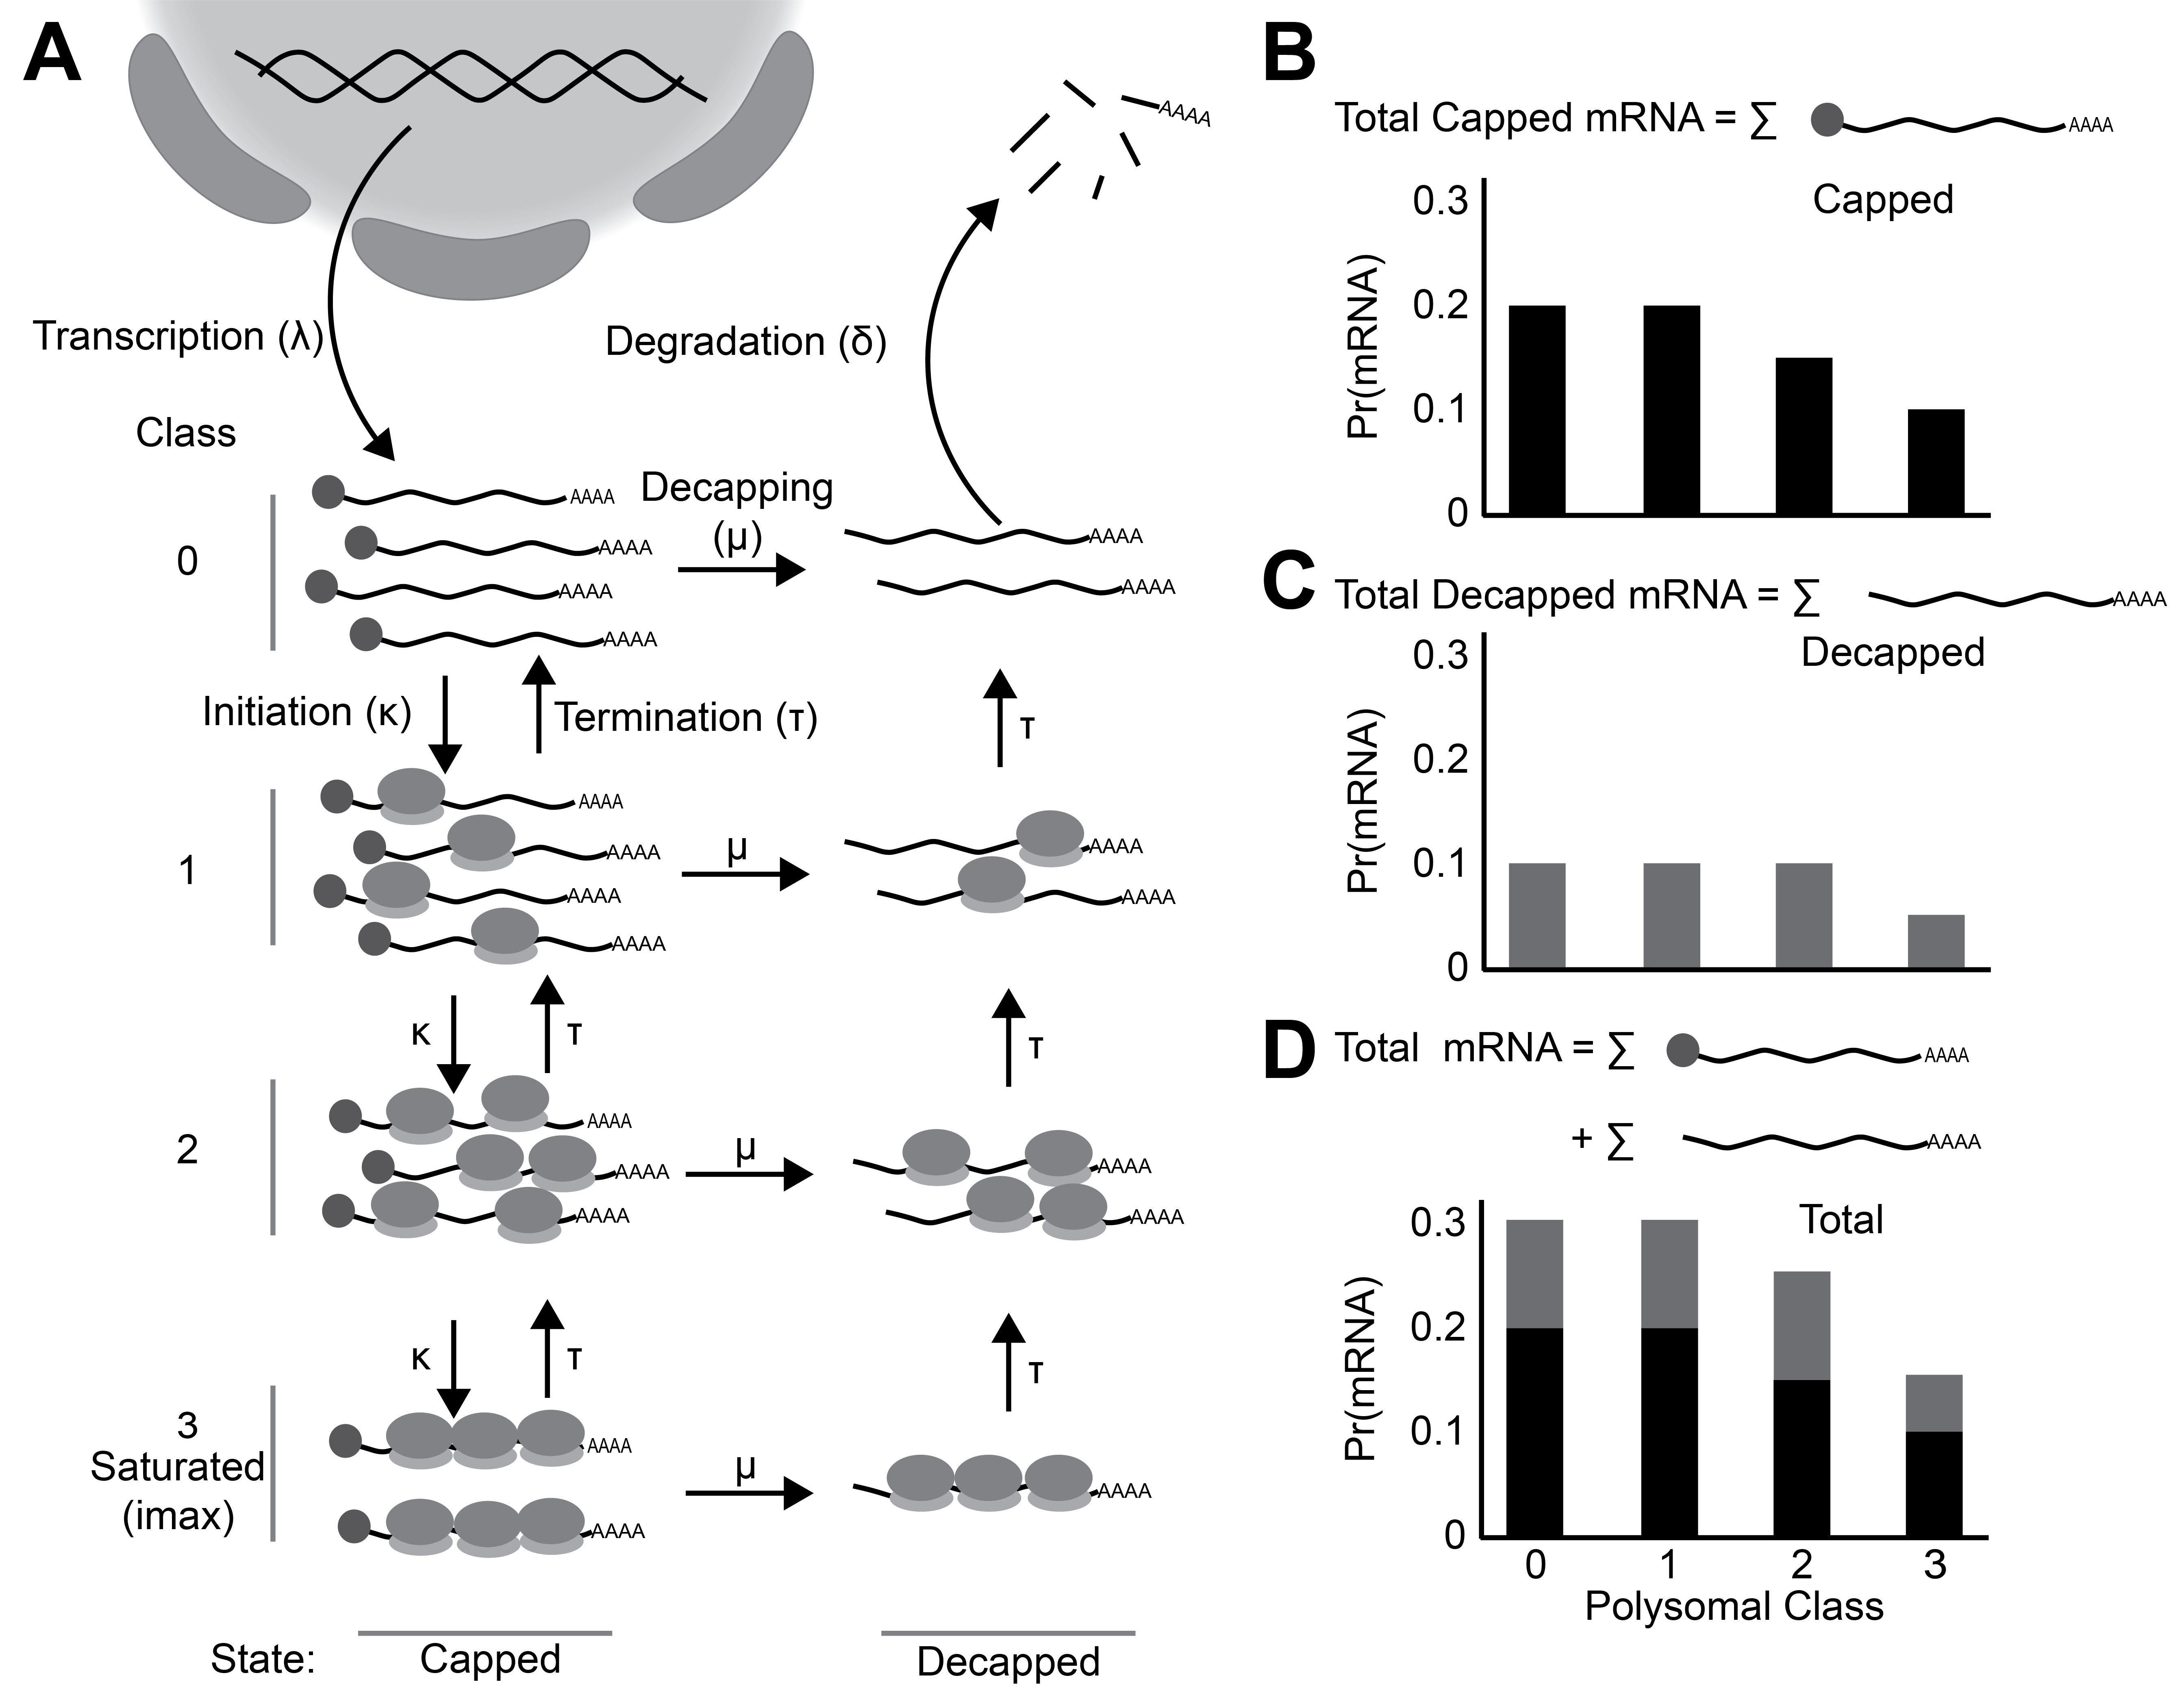
\includegraphics[width=150mm]{Images/Figure1_biomodel_V3.png}
\caption{Cartoon Representation of model in biological context. A) Model overview. Transcripts enter the sytem into the capped state at class 0 (no ribosomes bound). They enter the state at rate $\lambda$ through transcription. Transcripts are free to move up and down ribosomal classes at rates $\kappa$ for translation initiation and $\tau$ for elongation/termination. Transcripts can also be decapped and enter the decapped state at rate $\mu$. Finally, upon reaching class 0 in the decapped state transcripts are fully degraded at rate $\delta$. B) Probability of finding an mRNA in each class in the capped state. C) probability of finding an mRNA in each class in the decapped state. D) Joint probabilty of finding an mRNA in each class across each state. This reflect the total protein production potential.}
\end{figure}
\clearpage


The model captures some of the basic processes governing mRNA populations: transcript production, degradation and the process of translation (Figure 1A).
Transcripts can exist in one of two states: capped and decapped which captures the the role of the 5' cap in mRNA protection and translation initiation. 
Capped transcripts are translationally competent, meaning that new ribosome can be loaded onto the transcript. 
Individual transcripts in the cell will be found with a set number of ribosomes (none, 1, 2, etc).
The number of ribosomes on a transcript determines that transcripts polysomal class.
The model seeks to determine how the population of transcripts of a single gene are distributed between ribosomal classes and capped and decapped states.

Transcripts enter into the model as defined by the transcription rate $\lambda$ into the capped state with no ribosomes (polysome class 0)
From capped class 0 a transcript can have two fates. 
The transcript can be decapped, thus marked for degradation at rate $\mu$ and move into the decapped class 0.
Alternatively, a ribosome can initiate translation on the mRNAs in the capped, ribosome free polysome class 0 at rate $\kappa$ and be loaded onto the transcript and move it into capped class 1.
Because only one ribosomes can occupy a particular location on the mRNA at any given time and our model does not track ribosomal positions,
, we model translation intiation across polysome classes $i = 0$ to $\imax$, more generally as
\begin{equation}
  \label{eq:kappa_i}
  \kappa_i = \kappa_0 \left(1- \frac{i}{\imax}\right),
\end{equation}
where $i$ is the mRNA polysome class, \imax is the maximal ribosomal occupancy on the transcript.
We note $i/\imax$ represents, under the assumptions of a uniform distribution,  the probability a randomly chosen codon position is occupied by a ribosome.
Correspondingly, $(1 - i/\imax)$ represents probability a randomly chose codon position, such as the initiation site is unoccupied.
Because, the natural units for mRNA coding sequence length in our model is the amount of space the bound ribosome takes when translating it follows that $\imax = n_{c}/9$ where $n_{c}$ is the length of the mRNA's coding sequence in codons and 9 represents the length in codons of space a single ribosome occupies.
%$\imax = n_{\text{nt}}/27$ where $n_{\text{nt}}$ is the length of the mRNA's coding sequence in nucleotides.
This attempts to account for the ribosomal density dependent effects on initiation and is called the density dependent initiation (DDI) model.


A ribosome on the transcript elongates the peptide and, in turn, terminates at a rate of $\tau$, 
Given that the length scale of our model is formulated in terms of ribosome widths but most estimates of elongation are at the scale of codons, if $\tau_c$ is the average elongation rate of an mRNA in codons, $\tau = \tau_c/9$.
As the number of ribosomes on a transcript increase, the probability of a ribosome being at the end of the transcript also increases.
Again assuming ribosomes are distributed across a transcript according to a uniform distribution, the expected ribosome termination rate on a mRNA in polysome class $i$ is simply, 
\begin{equation}
	\tau_i = \tau \frac{i}{\imax}.
\end{equation}


Capped transcripts move through rounds of translation initiation and elongation-termination and distribute along the different polysomal classes. 
From any ribosomal class in the capped state the transcript can be decapped at rate $\mu$  and move into the decapped state while maintaining the same polysomal class.
Decapped transcripts can no longer initiate new rounds of translation, but allow for currently loaded ribosomes to complete translation. 
This process represent co-translational decay, a common method of mRNA decay in eukaryotes (Hu 2009, Pelechano 2015, Collart 2020) 
After all ribosome complete translation, the mRNA is in decapped class 0 and completely degraded at a rate $\delta$.
The model produces two outputs. 
First, the total mRNA in each state and therefore the system (Figure 1B-D). 
Second, The distribution of the mRNAs in each mRNA in each ribosomal class. (Figure 1 B-D).
The total protein output at steady state from our model can be obtained by calculating the average ribosomal class in the system by the total mRNA in the system (Figure 1D). 

\subsection{Formal Model Definition}
We formalize the DDI model presented in Figure 1 by converting each state in to a series of ordinary differential equations (ODEs) representing the mRNA population for each polysomal class. 
The functional form of the capped mRNA sub population is:
\begin{align} \label{eq:Capped_ODE}
\frac{dm_{0}}{dt} &= \lambda+ \tau \frac{1}{\imax}m_{1}-\left(\kappa_0 + \mu\right)m_{0} \\ \nonumber
\frac{dm_{1}}{dt} &= \kappa_0 m_{0}+ \tau \frac{2}{\imax}m_{2}-\left( \tau \frac{1}{\imax}+\kappa_0\left(1-\frac{1}{\imax}\right)+\mu\right) m_{1}\\ \nonumber
& \vdots & \\ \nonumber
\frac{dm_{i}}{dt} &= \kappa0 \left(\frac{i-1}{\imax}\right) m_{i-1}+ \tau \frac{i+1}{\imax}m_{i+1}-\left( \tau \frac{i}{\imax}+\kappa_0\left(1-\frac{i}{\imax}\right)+\mu\right) m_{i} \\ \nonumber
& \vdots & \\ \nonumber
\frac{dm_{\imax}}{dt} &= \kappa_0\left(1-\frac{\imax-1}{\imax}\right)m_{\imax-1}-\left( \tau +\mu\right) m_{\imax}\\ \nonumber
\end{align}

Similarly, the functional form of the decapped mRNA sub population is: 
\begin{align}\label{eq:Decapped_ODE}
\frac{dm_{0}^{*}}{dt} &= \mu m_{0}+ \tau \frac{1}{\imax}m_{1}^{*}-\delta m_{0}^{*} \\ \nonumber
\frac{dm_{1}^{*}}{dt} &= \mu m_{1}+ \tau \frac{2}{\imax}m_{2}^{*}-\tau(1)m_{1}^{*} \\ \nonumber
& \vdots & \\ \nonumber
\frac{dm_{i}^{*}}{dt} &= \mu m_{i}+ \tau \frac{i+1}{\imax}m_{i+1}^{*}-\tau(i)m_{i}^{*} \\ \nonumber
& \vdots & \\ \nonumber
\frac{dm_{\imax}^{*}}{dt} &= \mu m_{\imax}^{*}- \tau m_{\imax}. \\ \nonumber
\end{align}
In closing, we note the parameters $\imax, \kappa, \mu,$ and $\tau$ likely vary between genes.

\begin{table}
\centering
\begin{tabular}{|rp{4in}|c|c|c|}\hline
\textbf{Symbol}&\textbf{Description}&\textbf{Unit} \\\hline
State Variables & &  \\ \hline
$m_i$ & Abundance of mRNAs with a ribosome load of $i$ in capped state. & $mRNA$ \\
$m_i^*$ & Abundance of mRNAs with a ribosome load of $i$ in decapped state. & $mRNA$ \\ \hline
\multicolumn{1}{l}{Model Parameters} \\ \hline
i & ribosomal load index & Ribosome\\
  \imax & \shortstack{Maximum number of ribosomes able to bind to mRNA;\\
           defines number of state variables and is a function of gene length.} & Ribosome \\
$\kappa(i)$ & Translation initiation rate for unmarked mRNAs with a ribosome load of $i$. & $1/s$\\
$\tau(i)$ & Translation completion rate for the marked and unmarked mRNAs with a ribosome load of $i$. & $1/s$\\
$\mu(i)$ & decapping rate for unmarked mRNAs with a ribosome load of $i$. & $1/s$\\
$\lambda$ & Production rate of newly produced, ribosome free, and unmarked mRNA to the $m_0$ class. & $mRNA/s$\\
$\delta$ & Removal rate of marked mRNA with a ribosome load of 0 from the $m_0^*$ class. & $1/s$\\ \hline 
%\multicolumn{3}{|p{450pt}|}{\footnotesize Note: $\mathbb{R}^+$ represents the non-negative real numbers and $\mathbb{Z}^{(+)}$ represents the strictly positive integers.} \\ \hline
\end{tabular}
\caption{State variables and model parameters for ODE model of mRNA populations.
Variable \imax is in the domain of non-negative integers; all other variables are non-negative real numbers.}
\label{tab:params}
\end{table}

\subsubsection{Analytical steady state solutions of the capped transcript population}
Analytical exploration of the model's capped system presents no closed form solution for the capped system.
However, the model solution can be represented in the following form,
	\begin{equation} \label{eq:capped_solution}
		\vec{m}=\frac{\lambda}{\mu}\vec{p}_m
	\end{equation}
Where $\vec{m}$ is a vector of the steady state mRNA abundances in each polysomal class.
$\vec{m}$ is calculated from by scaling  the vector $\vec{p}$, which represents the distribution of the mRNA across the polysomal classes, by transcript production rate $\lambda$ and the decapping rate $\mu$ scale s.
While the individual components of $\vec{p}$ are functions of $i$, \imax, the translation initiation rate $\kappa$, the elongation rate $\tau_0$ and $\mu$ and have no closed form solution, it is worth noting that because the probability distribution of the capped population must sum to 1, by definition, it follows that
\begin{equation}\label{eq:capped_sum}
\sum_{i = 0} ^\imax m_i = \lambda/\mu.
\end{equation}

\subsubsection{Analytical steady state solutions of the decapped transcript population}

The solution for the decapped system is dependent on the underlying distribution of the capped system and can be represented as:

\begin{align*}
m_{0}^{*}  &= \frac{\mu}{\delta}\sum_{j=0}^{\imax}m_{j} \\
m_{1}^{*}  &= \frac{\mu}{\tau}\sum_{j=1}^{\imax}m_{j}  \\
& \vdots & \\
m_{i}^{*}  &= \frac{\mu}{i \: \tau}\sum_{j=i}^{\imax}m_{j}  \\
& \vdots & \\
m_{\imax}^{*}  &= \frac{\mu}{\imax \: \tau}\sum_{j=\imax}^{\imax}m_{j}  \\
\end{align*}
We can simplify the model by converting the mRNA quantity $m_{j}$ to the probability $p_{j}$ by ~\ref{eq:capped_solution}.
Additionally, for any $i=j$ where $S_{j}$ is cumulative probability from $i$ = class $j$ to $ i= \imax$.
\begin{equation}
		S_{j} = \sum_{i=j}^{\imax}\vec{p_{i}}
\end{equation}

Now the solution becomes,

\begin{align} \label{eq:decapped_solution} 
m_{0}^{*}  &= \frac{\lambda}{\delta}S_{0}=\frac{\lambda}{\delta} \\ \nonumber
m_{1}^{*}  &= \frac{\lambda}{\tau}S_{1} \\ \nonumber
& \vdots & \\ \nonumber
m_{i}^{*}  &= \frac{\lambda}{i \: \tau}S_{i}  \\ \nonumber
& \vdots & \\ \nonumber
m_{\imax}^{*}  &= \frac{\lambda}{\imax \: \tau}S_{\imax}  \\ \nonumber
\end{align}
 Note that $S_{0}=1$ and $ S_{0} \ge S_{1} \ge ... \ge S_{i} \ge ... \ge S_{\imax}$ dependant on the distribution of \mvechat of the capped state. %The pattern of  the  $S$ means that $m_0 \ge m_1 \ge ... \ge ... m_i \ge ... \ge m_imax$.

\subsection{Calculation of the decapped mRNA population}

The total transcript population in the decapped state does not have a closed form solution. However it can be summarized as follows,

\begin{equation*}
	m_{tot}^{*} = \sum_{i=0}^{\imax} m_{i}^{*} = \frac{\lambda}{\delta} + \frac{\lambda}{\tau}S_{1} + \hdots + \frac{\lambda}{i \tau}S_{i} + \hdots  + \frac{\lambda}{\imax \tau}S_{\imax} 
\end{equation*}
This can be further shortened to:
\begin{equation} \label{eq: marked_total_pop}
	m_{tot}^{*} = \lambda(\frac{1}{\delta} + \frac{1}{\tau}\vec{S} \cdot \vec{l}	) 
\end{equation}
Where $\vec{S}$ is a vector of all the cumulative sums and $\vec{l}$ is a vector of $1,1/2,...,1/i,...,1/\imax$ . 

\subsection{Probability distribution in the decapped state}

To get the probability distribution of transcripts across the decapped state we can divide $\vec{m^{*}}/m_{tot}^{*}$ which results in,
\begin{align}\label{eq:decapped_distribution}
	p_{0}^{*} &= \frac{1}{1 + \frac{\delta}{\tau}\vec{S} \cdot \vec{l}}	\\
  	p_{j}^{*} &= \frac{S_{j}}{j(\frac{\tau}{\delta} + \vec{S} \cdot \vec{l})}	\:\:\:\: \text{for } j=1, 2, ..., i, ..., \imax
\end{align}

\subsection{Calculation of the total mRNA population and its distribution between capped and decapped states}
The total mRNA ($M_{tot}$) in the system is defined by,
\begin{equation}
	M_{tot} = \frac{\lambda}{\mu} +  \lambda(\frac{1}{\delta} + \frac{1}{\tau}\vec{S} \cdot \vec{l})
\end{equation}

To understand how mRNA is divided  between we start with the probability of finding an mRNA in the capped state.
\begin{equation*}
	p_{mtot} = \frac{1}{(1  + \frac{\mu}{\delta} + \frac{\mu}{\tau}\vec{S} \cdot \vec{l})}	
\end{equation*}
Then you calculate the odds,
\begin{equation}\label{eq:odds}
	odds_{\hat{m}} = \frac{1}{\mu(\frac{1}{\delta} + \frac{1}{\tau}\vec{S} \cdot \vec{l}} )\\
\end{equation}


\subsection{Calculating expected ribosomal load and protein production}
The expected ribosomal load for either the capped or decapped state is calculated by:
\begin{equation}\label{eq:Expected_ribo_load}
	E(ribosome) =\sum_{i=0}^{\imax}j\times p_{i}
\end{equation}
Where $\vec{p_m}$ is the distribution in either state and i is the polysome class.

To find the global mean ribosomal load we obtain,
\begin{equation}\label{eq:System_ribo_load}
	\text{Total Ribosomal Load} = p_{mtot}\times E(ribosome)_{mtot} + (1-p_{mtot})\times E(ribosome)_{mtot^*}
\end{equation}

\subsection{Numerical solution implementation in R}
Code to solve the model was written in the R package Ribosome (\url{https://github.com/rurquidi/Ribosome}). To solve the capped subsystem of the model, the solve.tridiag algorithm from limSolve package (V 1.5.6) (Soetaert,K 2009). The decapped solution was obtained by using the capped solutions into ~\ref{eq:decapped_solution}. Utility functions, plots and statistics were created using  R (v 3.6) (R core team), and  data.table (v1.14.0) (Dowle 2021). 
		
\subsection{Data Sources}

In order to biologically contextualize and illustrate our model's behavior, we will focus on parameter ranges derived from the literature.
The range of \imax is determined from the distribution of protein lengths obtained from yeast (\textit{saccharomyces cerevisiae}) and the plant \textit{Arabidopsis thaliana}. To determine \imax, protein lengths are divided by the average number of codons covered by a ribosome, which is ~9 codons (Figure 2A and C). The range of \imax is  48 $\pm$ 36 for yeast and 47 $\pm$ 30 for Arabidopsis.
Protein lengths were extracted from the Ensembl (version 109) and Ensembl plants (version 56) respectively (Cunningham 2022, Yates 2022, Kinsella 2011).  
The decapping rate between the capped and uncapped system was approximated from the protein half-lives from Presnyak 2015 for yeast (Figure 2B) and Sorenson 2018 for Arabidopsis (Figure 2D).
We approximated gene specific $\mu$ from the half lives with the following:
	\begin{equation*}
		\mu_i = \frac{ln(2)}{t_{1/2_i}}
	\end{equation*}
Where $t_{1/2}$ is the half-life. The resulting range of $\mu$ is from $1.3 \times 10^-3 \pm 1.8 \times 10^-3$ for yeast and $1.7 \times 10^-4 \pm 2 \times 10^-4$ for Arabidopsis. 

Translation initiation and average elongation rates ($\kappa$ and $\tau_0$) were obtained for Yeast from Duc and Song 2018. In Duc and Song 2018, the authors used 850 highly translated transcripts from the ribo-seq dataset from Weinberg 2016. They employed a TASEP model to estimate the initiation rates and correct the empirical elongation rates from the footprint distributions. We calculated an average gene specific elongation rate from the corrected elongations rates. We scale the each gene specific initiation rate by dividing it by the gene specific elongation rate.
\begin{equation}
	\text{initiation to elongation ratio} = \kappa' = \frac{\kappa}{\tau_0}
\end{equation}

This simplifies the model behavior to one generalized parameter with a unique response (Figure 2E).  The initiation to elongation ratio ranges from 0.1$s^{-1}$ to 0.001$s^{-1}$.

The transcription rate, $\lambda$ only acts as a scaling factor throughout the model and does not affect the distribution of the ribosomes. For solutions provided in this work $\lambda$ has been set to one. However, as a point of reference, the transcriptomic results from Weinberg 2016 are included in Figure 2F. In short, reads per kilobase million from Weinberg were further converted into a log10 fold change based on the median expression level. Figure 2F shows that the absolute range of transcriptional expression ranges just under 5 orders of magnitude.

The mRNA clearance rate $\delta$ only determines the accumulation of transcripts in the  $m_0^*$  class, which for simplicity of interpreting results has been set to be $>>\tau$ and thus will not accumulate transcripts in $m_0^*$.
 
The empirical mean ribosomal load (MRL) for the 850 genes in Duc and song 2018 was calculated from the mRNA-seq read per kilbase million (mRNA RPKM) and the ribo-seq footprints (RPF RPKM) from Weinberg 2016. The following equation was used.
\begin{equation}\label{eq:MRL}
	MRL_i = \frac{RPF\: RPKM_i}{mRNA\: RPKM_i \times \frac{200}{length mRNA_i}}
\end{equation}

Where the gene specific scaling factor $\frac{200}{length mRNA_i}$ corrects for the bias in read counts due to longer transcripts producing more fragments. The value 200 arises from the average fragment size of a library prep and can be adjusted according the experimental method used.

\begin{figure}[!ht]
\centering
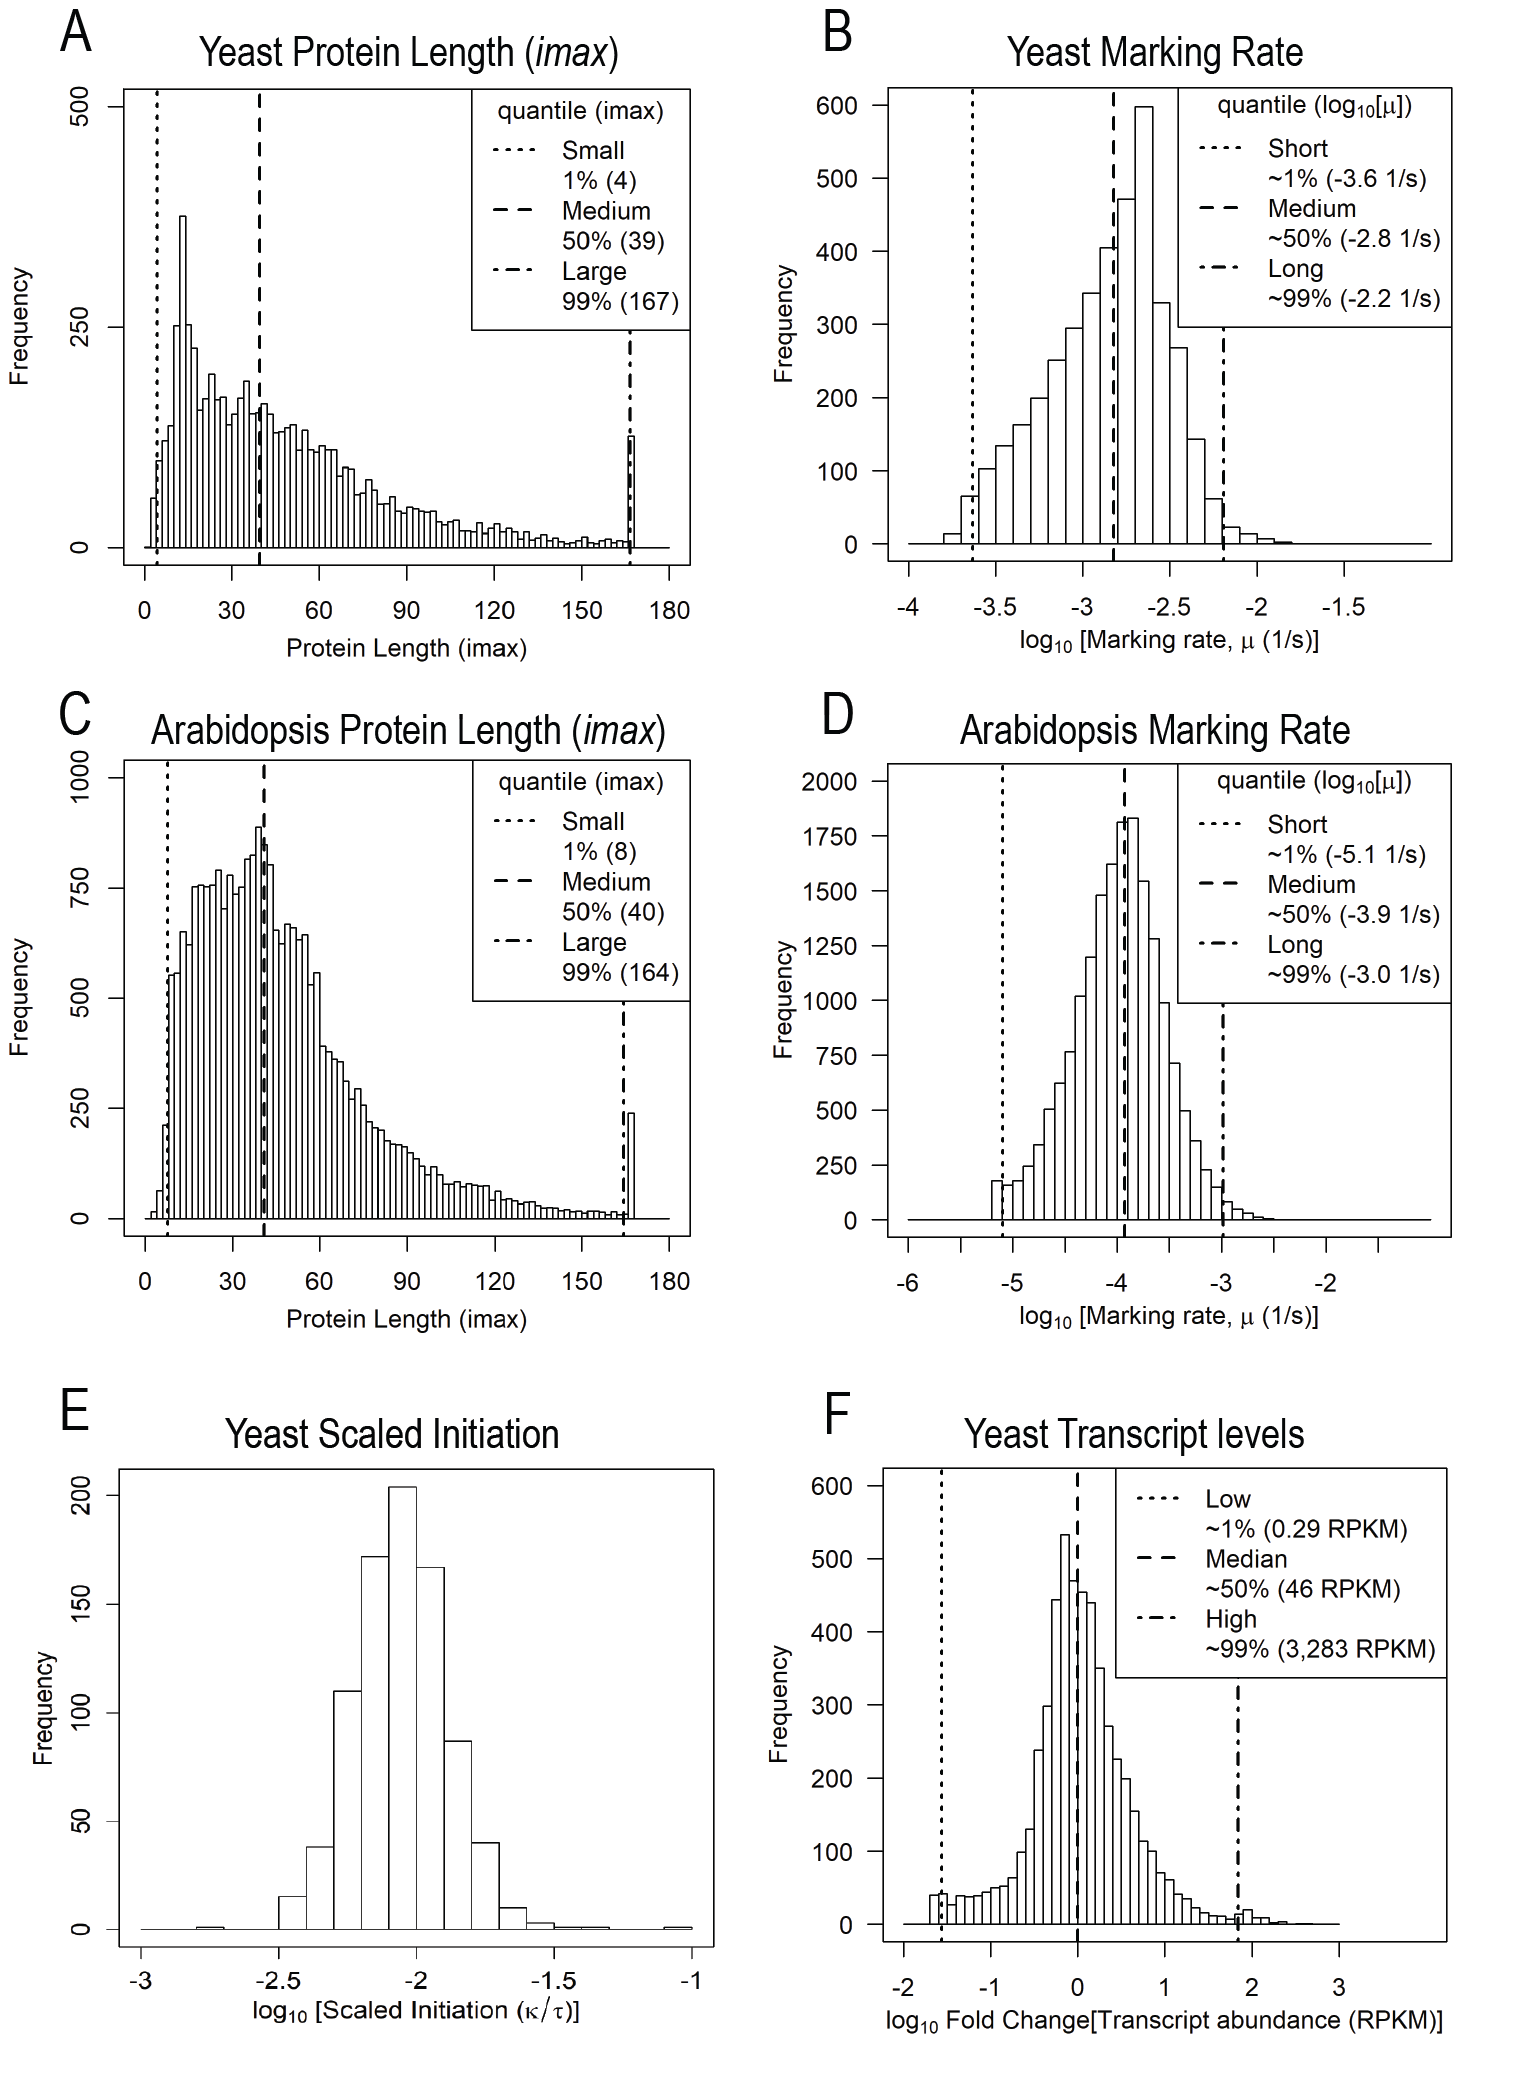
\includegraphics[width=120mm]{Images/2023-07-04_parameter_histograms.png}
\caption{Histograms of empirical values of model parameters. A) Yeast protein lengths. B) Yeast half-life C) Arabidopsis Protein Lengths. D) Arabidopsis Half-Life. E) Yeast Scaled elongation rates (Translational initiation rate/average translation elongation rate) on a per gene basis. F) Log 10 Fold Changes between all transcripts compared ot the median transcript expression in yeast. }
%\centering Red: de_s class, Green: capped class, Blue: Total= capped+decapped classes}
\end{figure}
\clearpage		


% It could be futher extended to include more degradations mechanisms see note below
% $\delta\ might be more complex with a slightly different model design. In the current model formulation it mimics the primary (but not only) degradation with the cell, the 5' decapping and subsequent VCS /XRN1 5'-3' cotranslation degradation system. This ignores 3 other systems the two 3'- 5' pathways (CCR4-NOT3) and exosome, and the final slew of endodegradation pathways (NGD, NSD, NMD, ribothrypsis, and silencing).
%Additionally, degradation of the bulk of the mRNA transcript might not be a process specific to each transcript (ie. due to coding sequence, I would have to look this up. Also might be testable with data fitting).


\section{Results}

\subsection{Model provides a unique distribution of mRNAs across polysome classes for each initiation to elongation ratio}
\begin{enumerate}
\item The model predicts the abundances of the mRNA in the capped and decapped states as well as the mRNA's distribution across polysome classes.
\begin{enumerate}
  \item Steady state solution of the capped class
  \begin{enumerate}
    \item The analytical steady state solution ~\ref{eq:capped_solution} is composed of a vector of probabilities $\vec{p_m}$ that an mRNA is in polysome class $i$ and a scaling term (the transcription rate $\lambda$ divided by the decapping rate $\mu$). 
    \item This solution highlights two separate roles of $\mu$.
    \begin{enumerate}
      \item First, the scaling term $\lambda / \mu$ determines mRNA abundance in the capped state.
      \item Second, the vector of probabilities is a function of the initiation rate $\kappa$, the elongation/termination rate $\tau$ and $\mu$ and is independent of $\lambda$.
    \end{enumerate} 
    \item Figure 3A shows the mRNA distribution in the capped state for four different initiation to elongation ratios $\kappa'$, for a protein of median length (\imax of 39) with a low decapping rate ($2\times10^{-4}$).
    \item To summarize the model results across a range of parameters a heatmap where each row is the steady state distribution of mRNA at a particular $\kappa'$ is shown (Figure 3B).
    \item  The steady state density in the capped system is bounded at class 0 and class \imax and can be roughly approximated by a truncated gaussian. 
    \item When $\kappa'<<\tau$, the distribution concentrates at low $i$ near the $i=0$ boundary.
    \item As $\kappa'$ increases, the steady state distribution moves towards higher $i$.
     \end{enumerate}
\begin{figure}[!ht]
\centering
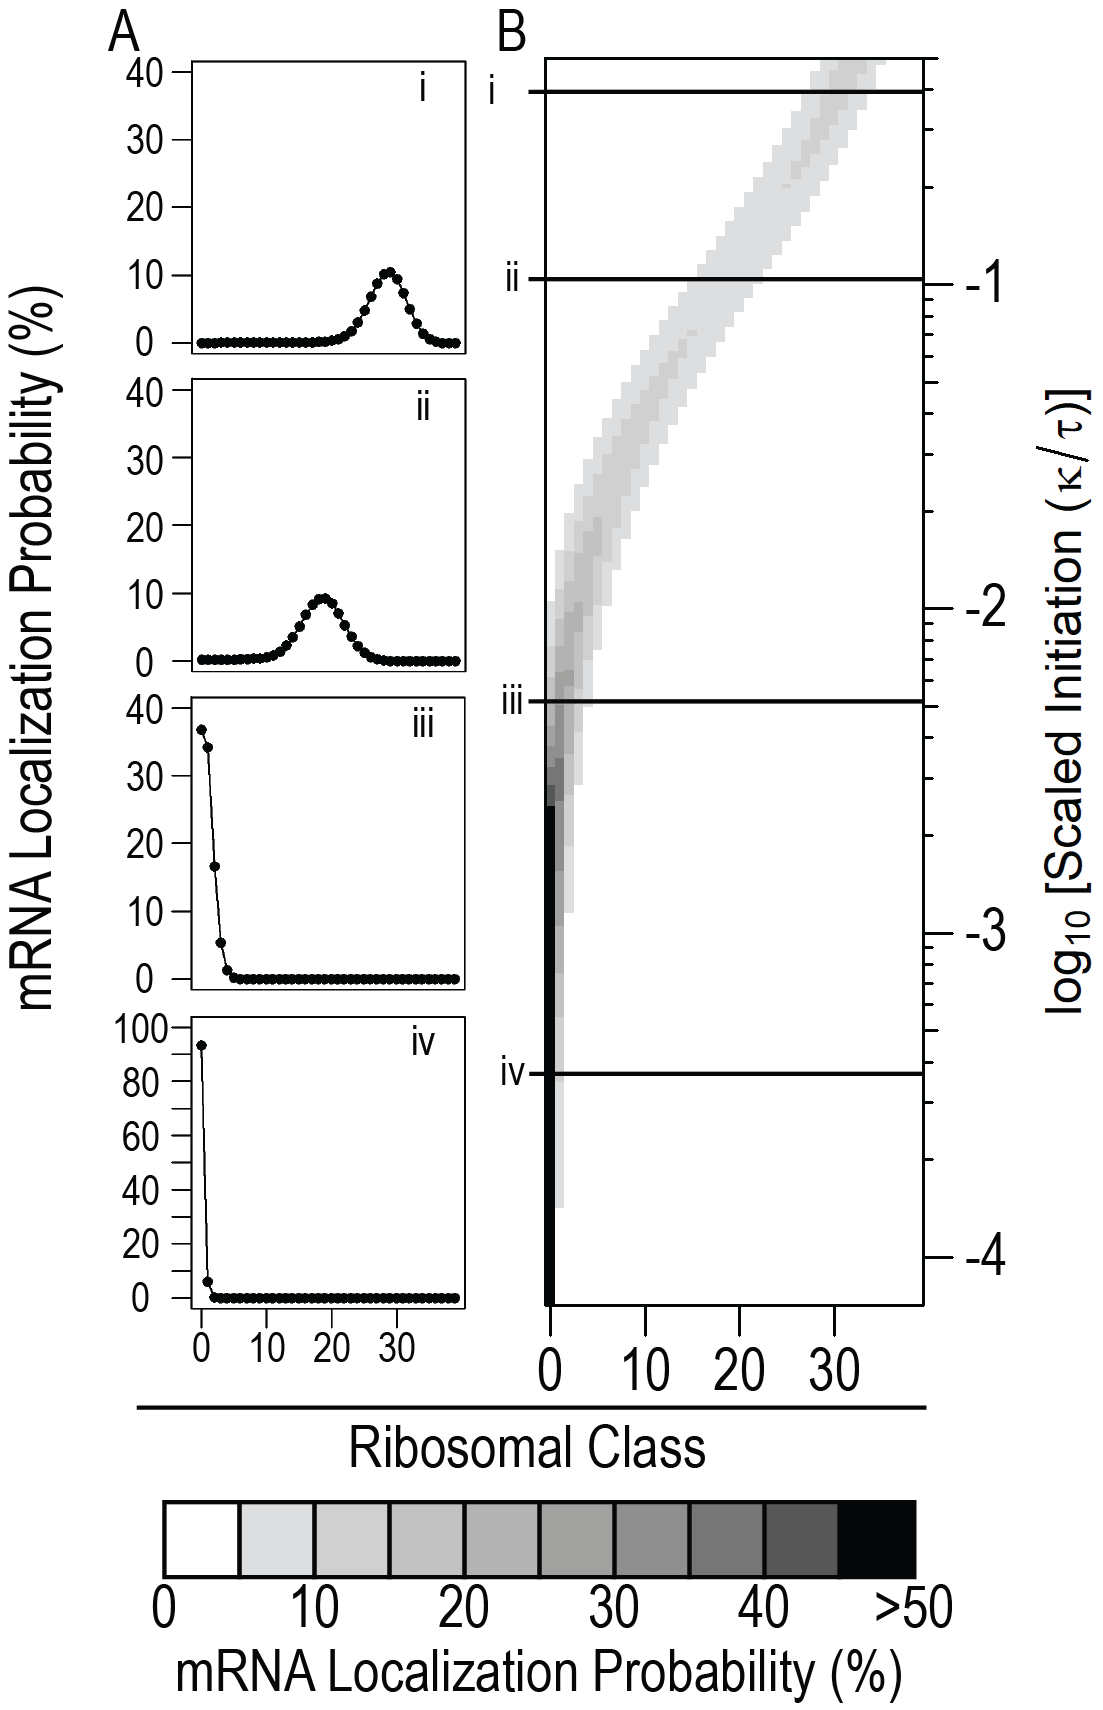
\includegraphics[width=100mm]{Images/2023-07-04_Unmarked_slices.png}
\caption{mRNA distribution in capped state. A) Distribution profiles for four scaled initiation values i) $2\times 10^{-1}$ ii) $1.03\times 10^{-1}$ iii) $3\times 10^{-3}$ iv) $2\times 10^{-4}$ B) Heatmap of model output across a range of scaled initiation values. Lines represent slice represented in A). Results produced with \imax of 39 and a low decapping rate of $2\times10^{-4}$  (99\textsuperscript{th} percentile). Color bar shows probability of finding mRNA in particular ribosomal class.}
%\centering Red: decapped class, Green: capped class, Blue: Total= capped+decapped classes}
\end{figure}
\clearpage

  \item  Steady state solution of the decapped class
  \begin{enumerate}
    \item The whole system is again scaled by the transcription rate $\lambda$.
    \item  The analytical steady state solution eq. ~\ref{eq:decapped_solution} can be understood in two parts. 
    \item $m_0^*$ and the remaining $m_i^*$ for $i>0$.
    \item $m_0^*$ is solely determined by the ratio of the mRNA clearance rate 1/$\delta$.
    \item The remaining decapped polysome classes depend on the elongation/termination rate $\tau$ and the distribution of \mvechat.
    \item  Figure 4A shows the mRNA distribution in the decapped state for four different initiation to elongation ratios $\kappa'$, for a median length protein with a low decapping rate ($2\times10^{-4}$) and the full range of $\kappa'$ are shown in the heatmap in Figure 4B.
     \item The mRNA distributions are centered around low $i$ and are monotonically decreasing. 
  \end{enumerate}	

\begin{figure}[!ht]
\centering
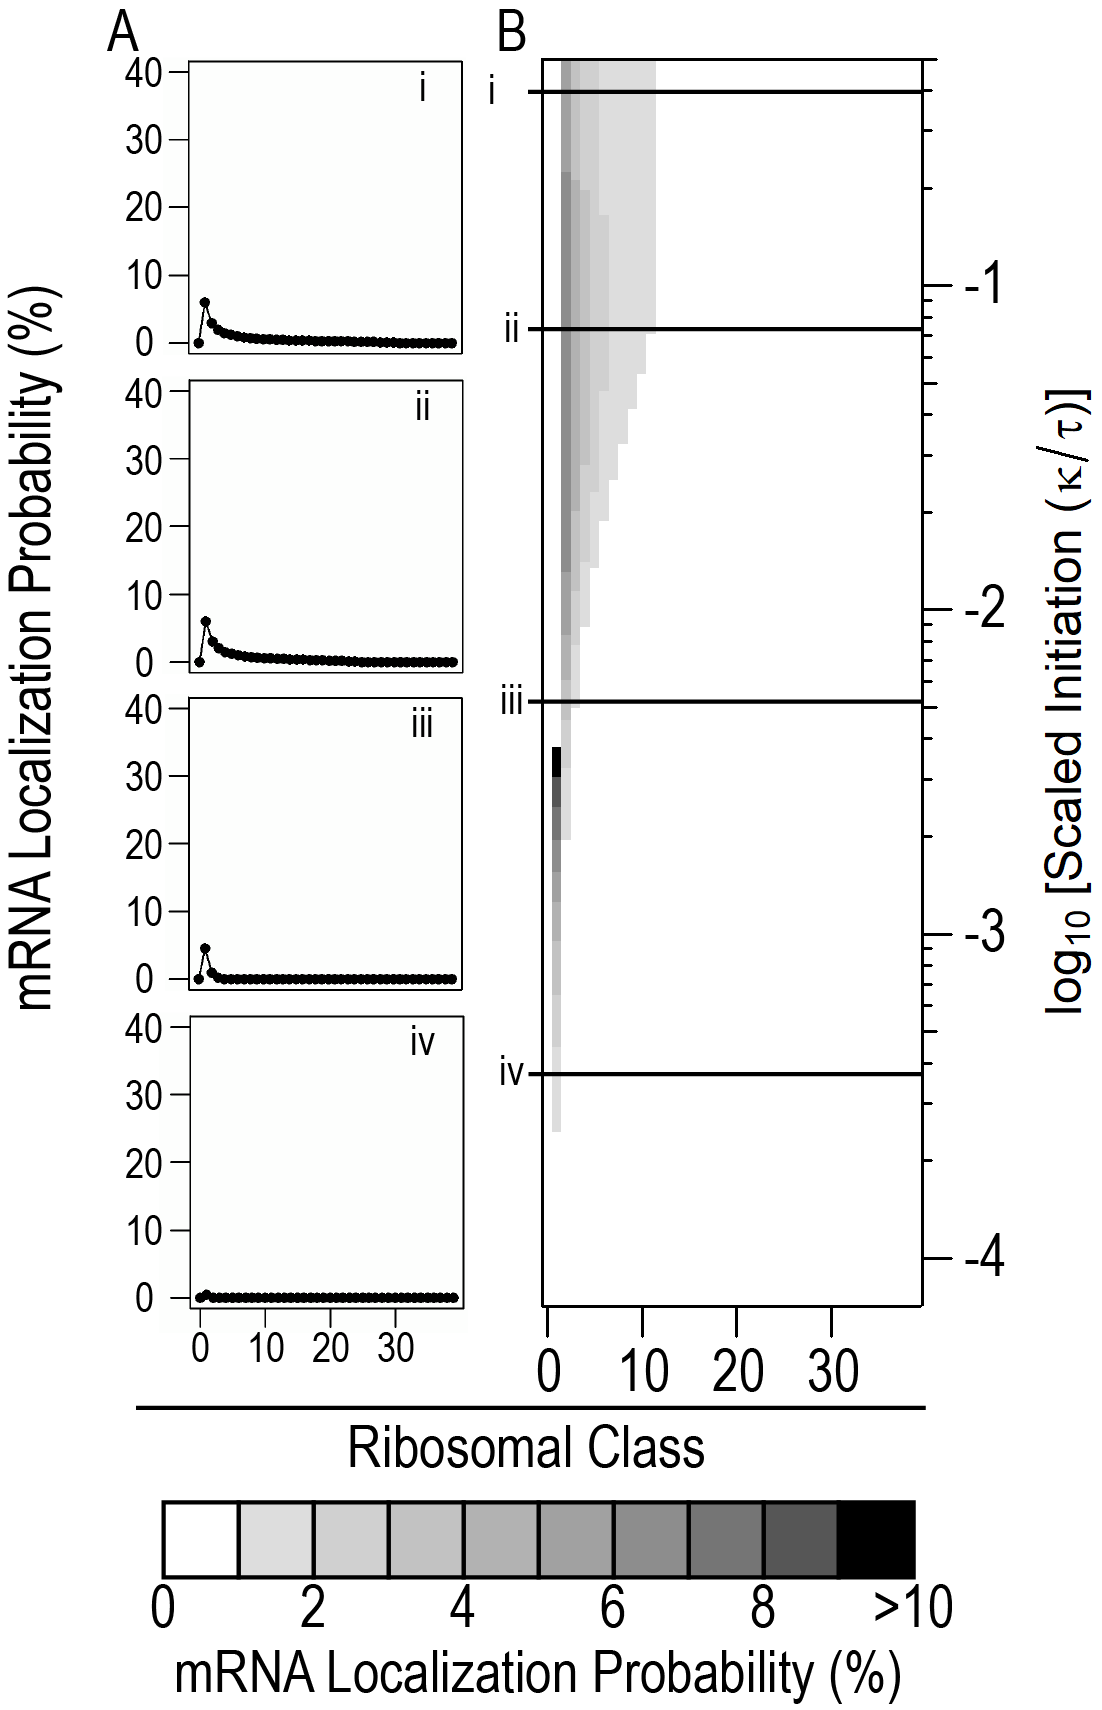
\includegraphics[width=100mm]{Images/2023-07-04_Marked_slices.png}
\caption{mRNA distribution in decapped state. A) Distribution profiles for four scaled initiation values i) $2\times 10^{-1}$ ii) $1.03\times 10^{-1}$ iii) $3\times 10^{-3}$ iv) $2\times 10^{-4}$ B) Heatmap of model output across a range of scaled initiation values. Lines represent slice represented in A). Results produced with \imax of 39 and a low decapping rate of $2\times10^{-4}$  (99\textsuperscript{th} percentile). Color bar shows probability of finding mRNA in particular ribosomal class.}
%\centering Red: decapped class, Green: capped class, Blue: Total= capped+decapped classes}
\end{figure}
\clearpage

  \item Steady states solution for the full model
  \begin{enumerate}
    \item The full model combines the mRNA distributions from the capped and decapped states.
    \begin{enumerate}
      \item Figure 5A shows the mRNA distribution in the full model for three values of $\kappa'$, for a median length protein with a low decapping rate ($2\times10^{-4}$) and the full range of $\kappa'$ are shown in the heatmap in Figure 5B.
      \item The system is unimodal at low $\kappa'<0.01$ when the capped and decapped distributions overlap around low $i$ (Figure 5A mid and low). 
      \item As $\kappa'>0.01$ increases, the full distribution becomes bimodal (Figure 5A high).
      \item The peak at low $i$ representing the decapped distribution, and the higher gaussian peak representing the capped distribution. 
    \end{enumerate}
  \end{enumerate}

\end{enumerate}

\end{enumerate}

\begin{figure}[!ht]
\centering
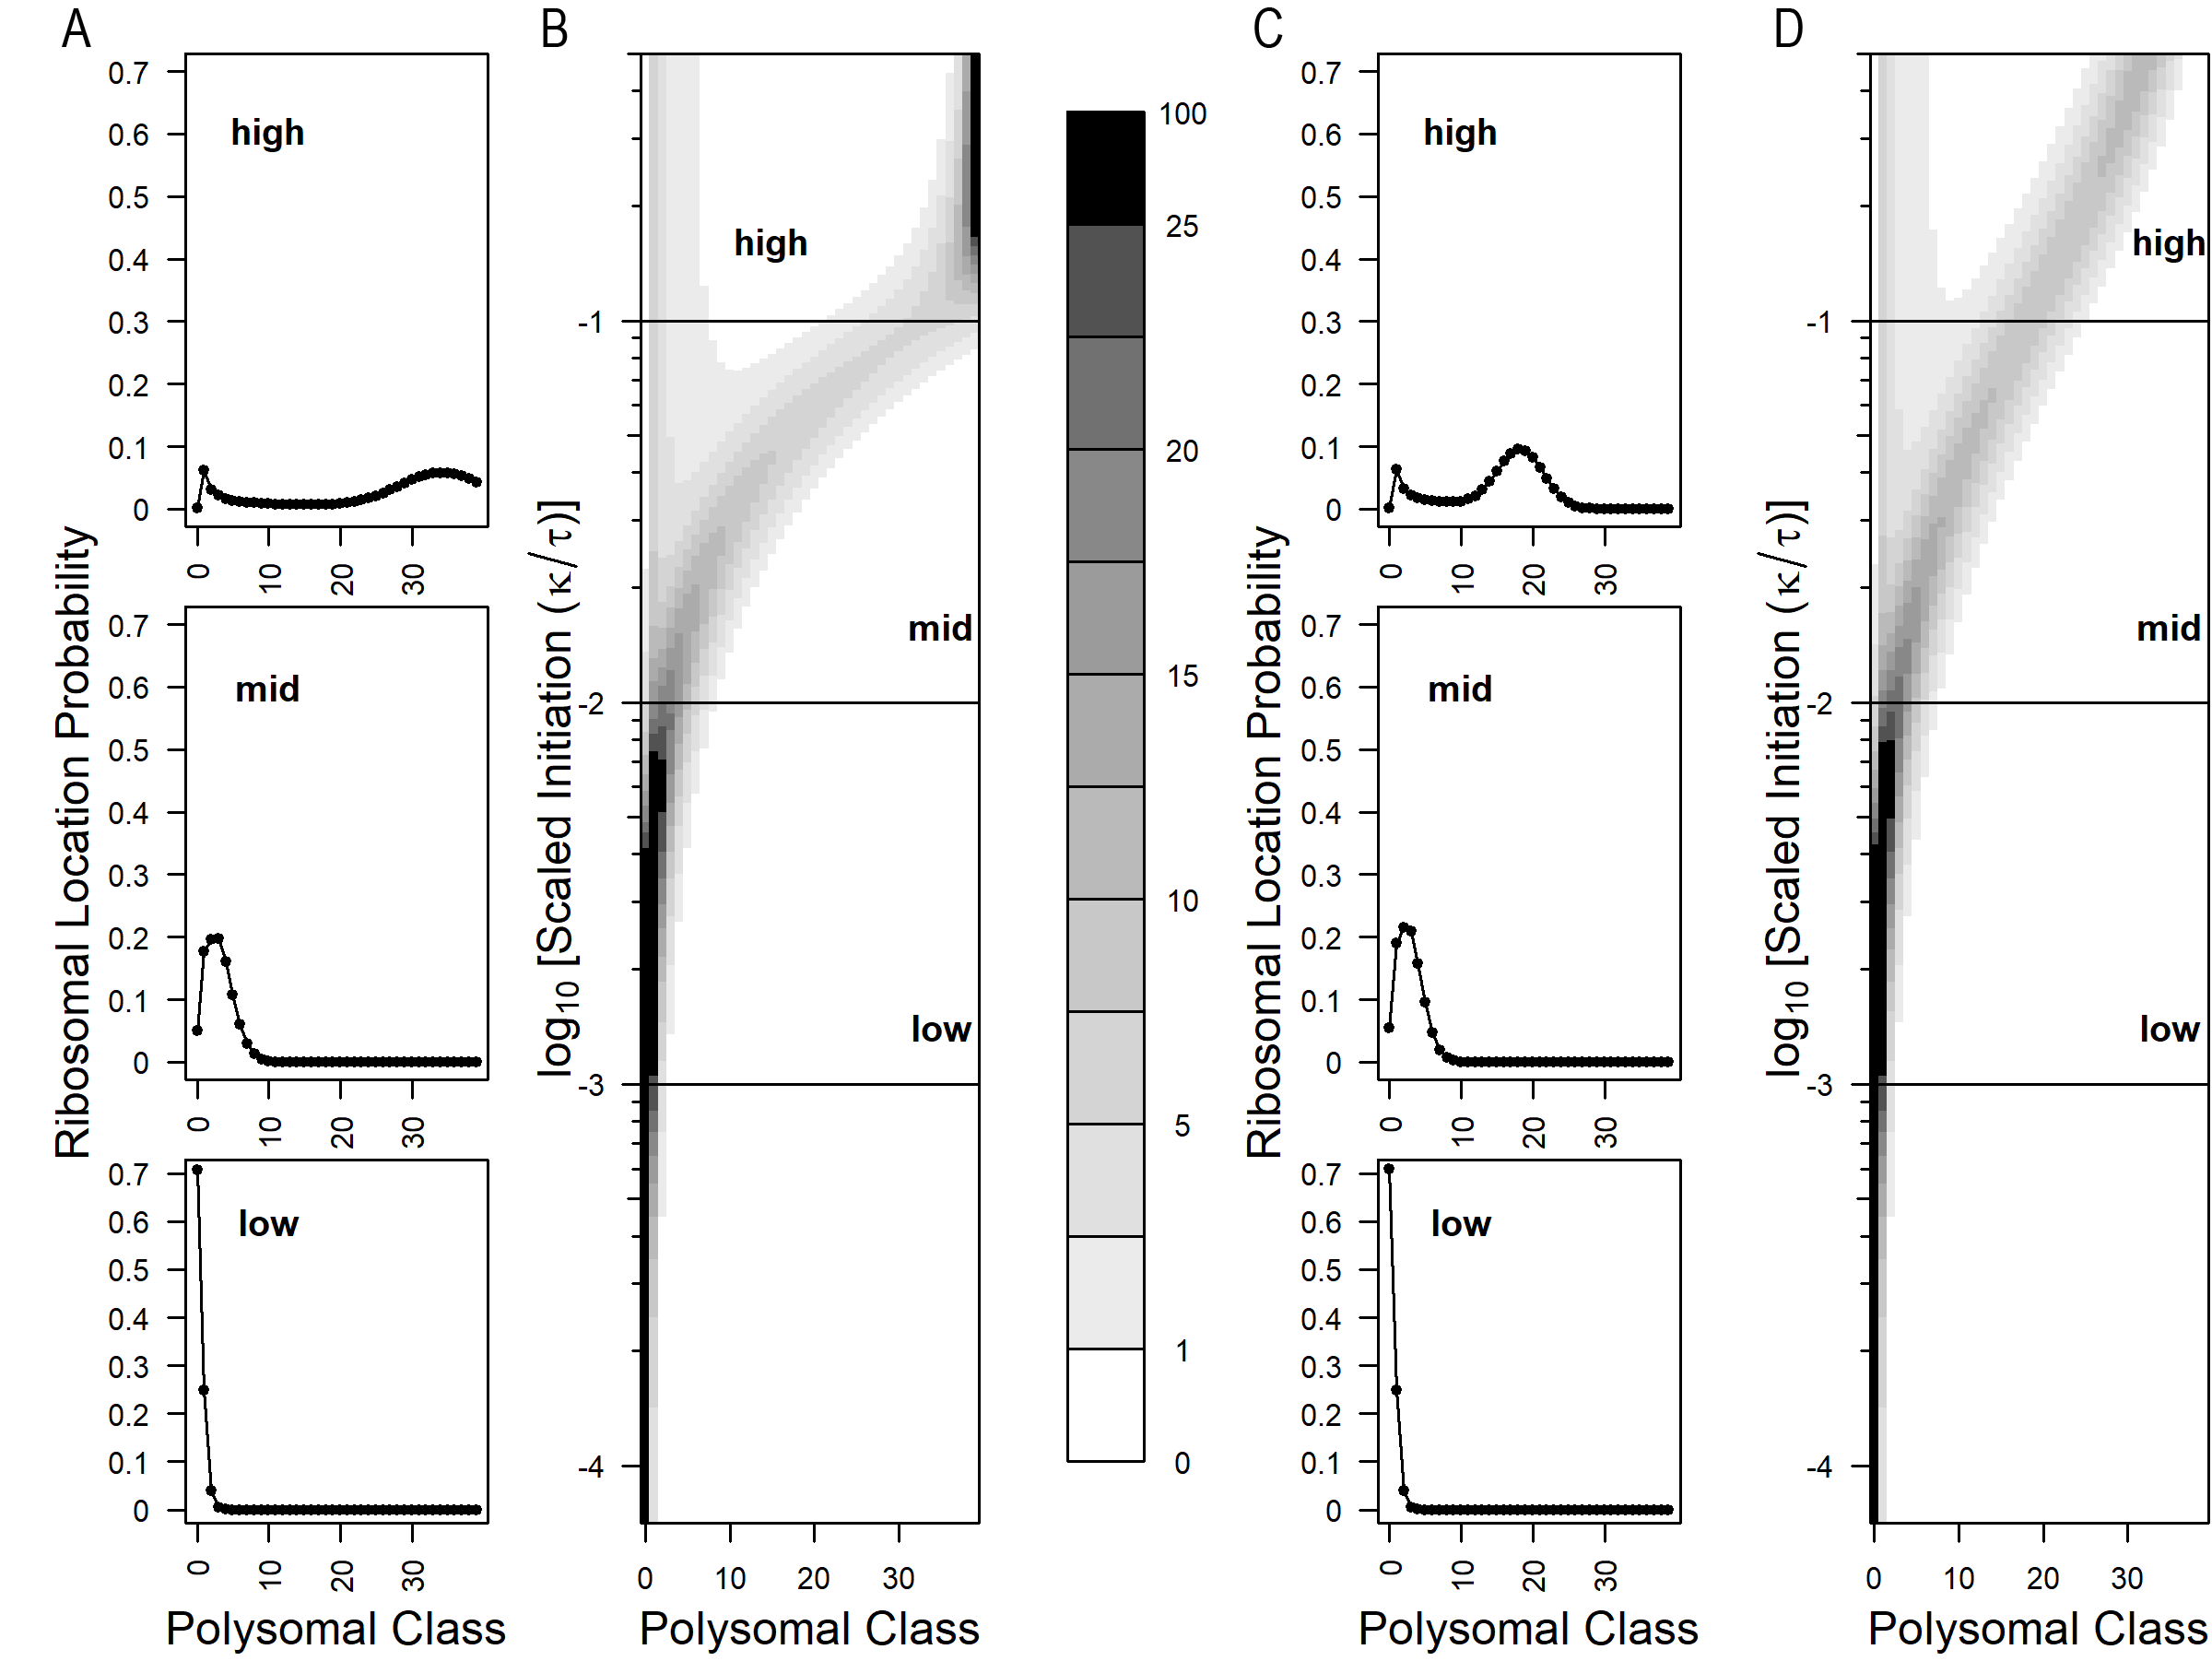
\includegraphics[width=120mm]{Images/2023-07-09_Figure1_DIIvsDDI_medianlength_low_marking_with_labels.png}
\caption{mRNA distribution in the full model. A) Distribution profiles for three scaled initiation values low) $1\times 10^{-3}$ mid) $2\times 10^{-2}$ and high) $1\times 10^{-1}$ B) Heatmap of model output across a range of scaled initiation values. Lines represent slice represented in A). Results produced with \imax of 39 and a low decapping rate of $2\times10^{-4}$  (99\textsuperscript{th} percentile). Color bar shows probability of finding mRNA in particular ribosomal class.}
%\centering Red: decapped class, Green: capped class, Blue: Total= capped+decapped classes}
\end{figure}
\clearpage


\subsection{Higher decapping rates reduce capped state ribosomal loads }
\begin{enumerate}
\item To explore the role of mRNA stability on mRNA populations we varied the decapping rate $\mu$ from the 1\textsuperscript{st}, 
\begin{enumerate}
  50\textsuperscript{th} and 99\textsuperscript{th} percentile values as determined from  Presnyak 2015.
  \item As $\mu$ increases the distribution of mRNAs changes in two ways. 
  \begin{enumerate}
     \item First there is shift to lower ribosomal classes in the capped state (Figure 6).
     \item This is likely due to the mRNAs leaving the capped state at a higher rate and driving the equilibrium towards lower ribosomal loads. 
     \item Secondly, as half-life decreases, a larger proportion of the mRNA is found in the decapped state. This is further explored later. 
  \end{enumerate}
\end{enumerate}
\begin{figure}[!ht]
\centering
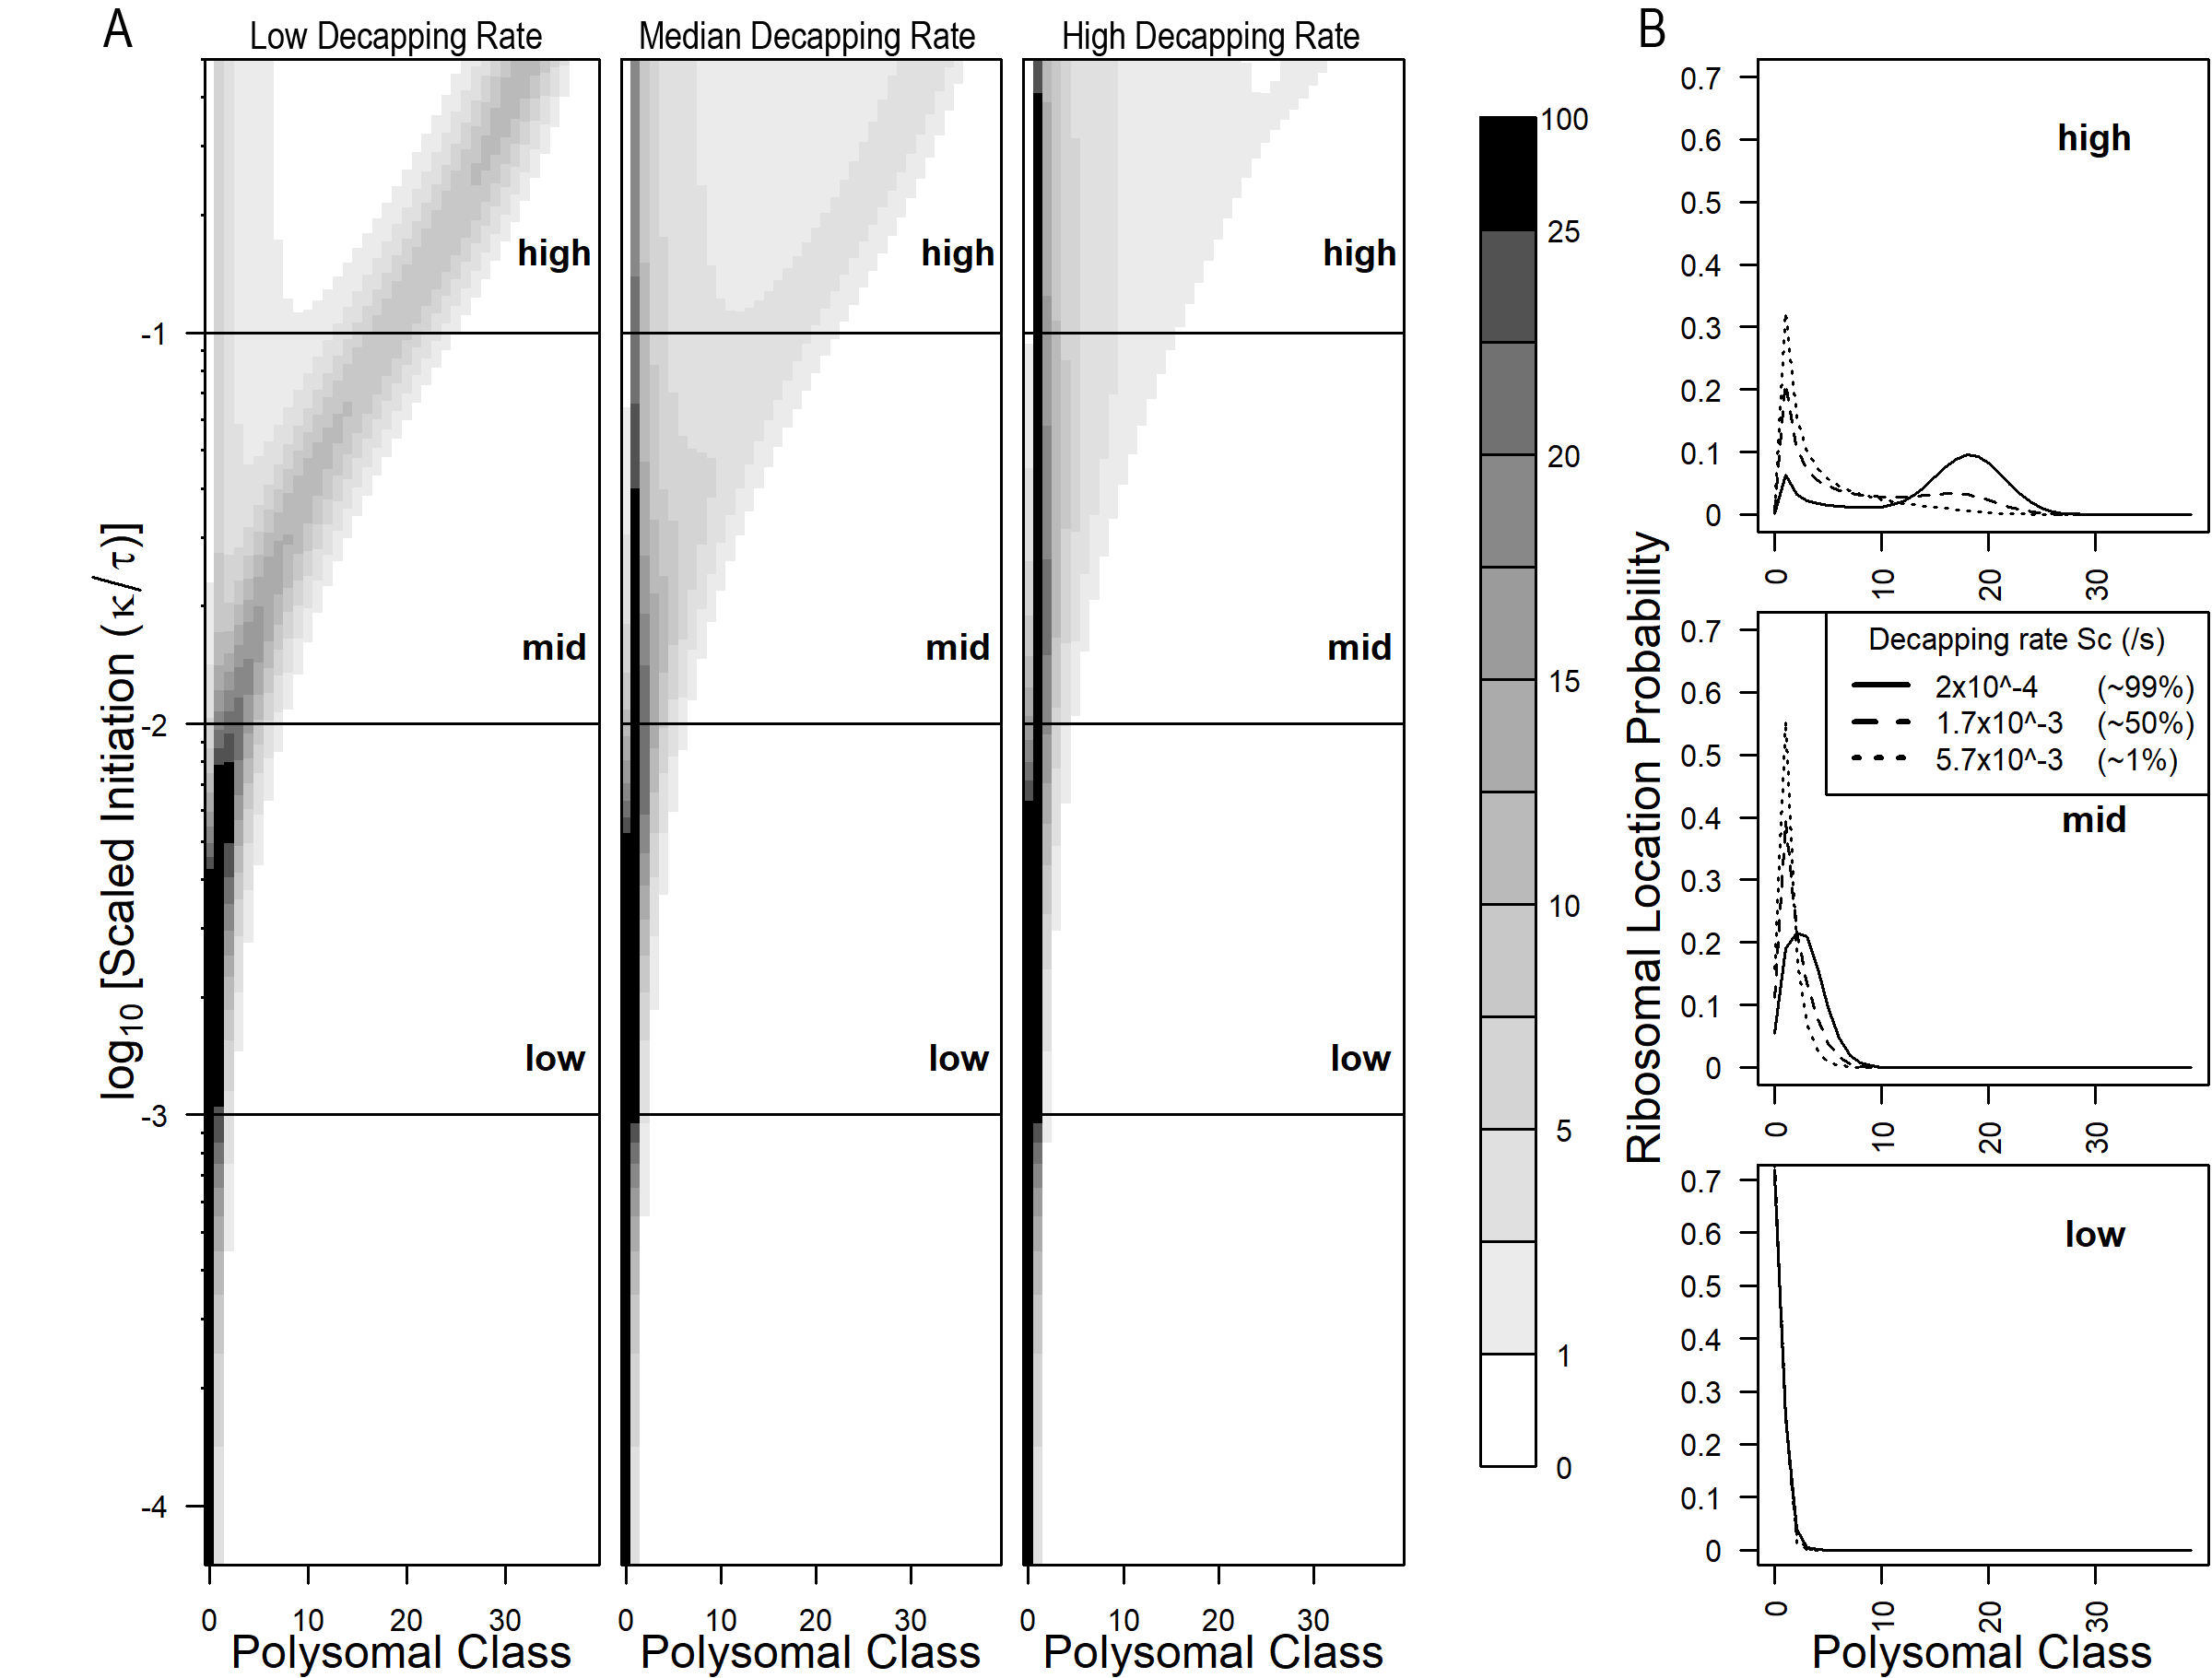
\includegraphics[width=120mm]{Images/2023-07-09_Figure2_Marking_Rate_range_medianlength_with_labels.png}
\caption{Higher decapping rates $\mu$ reduce ribosome load in the capped system in yeast.  A)  Heatmaps for the full model. Left) low $\mu$ ($2\times 10^{-4}$ /s) Center) median $\mu$ ($1.7\times 10^{-3}$ /s) Right) $\mu$ ($5.7\times 10^{-3}$ /s)  B) individual density profiles for low (0.001), mid (0.01) and high (0.1) scaled initiation values for each $\mu$ All results calculate with \imax = 39.}
%\centering Red: decapped class, Green: capped class, Blue: Total= capped+decapped classes}
\end{figure}
\clearpage

\item Plants and other multicellular eukaryotes tend to have slower translation initiation and elongation rates as well as slower cell division when compared to single celled organisms such as yeast.
\begin{enumerate}
  \item This is highlighted by the current gold standard study of mRNA half-lives in the model organism \textit{Arabidopsis thaliana}, where the decapping rate $\mu$ measured are ten to one hundred times lower than those in yeast. 
  \item To explore the effect of lower $\mu$ in Arabidopsis, we ran the model using the same initiation to elongation ratios as in yeast, the median Arabidopsis \imax of 41. 
  \item As expected, the longer half-lives have a higher mRNA distribution (Figure 7) and are mostly in the capped state (Figure 10).
\end{enumerate}
\end{enumerate}

\begin{figure}[!ht]
\centering
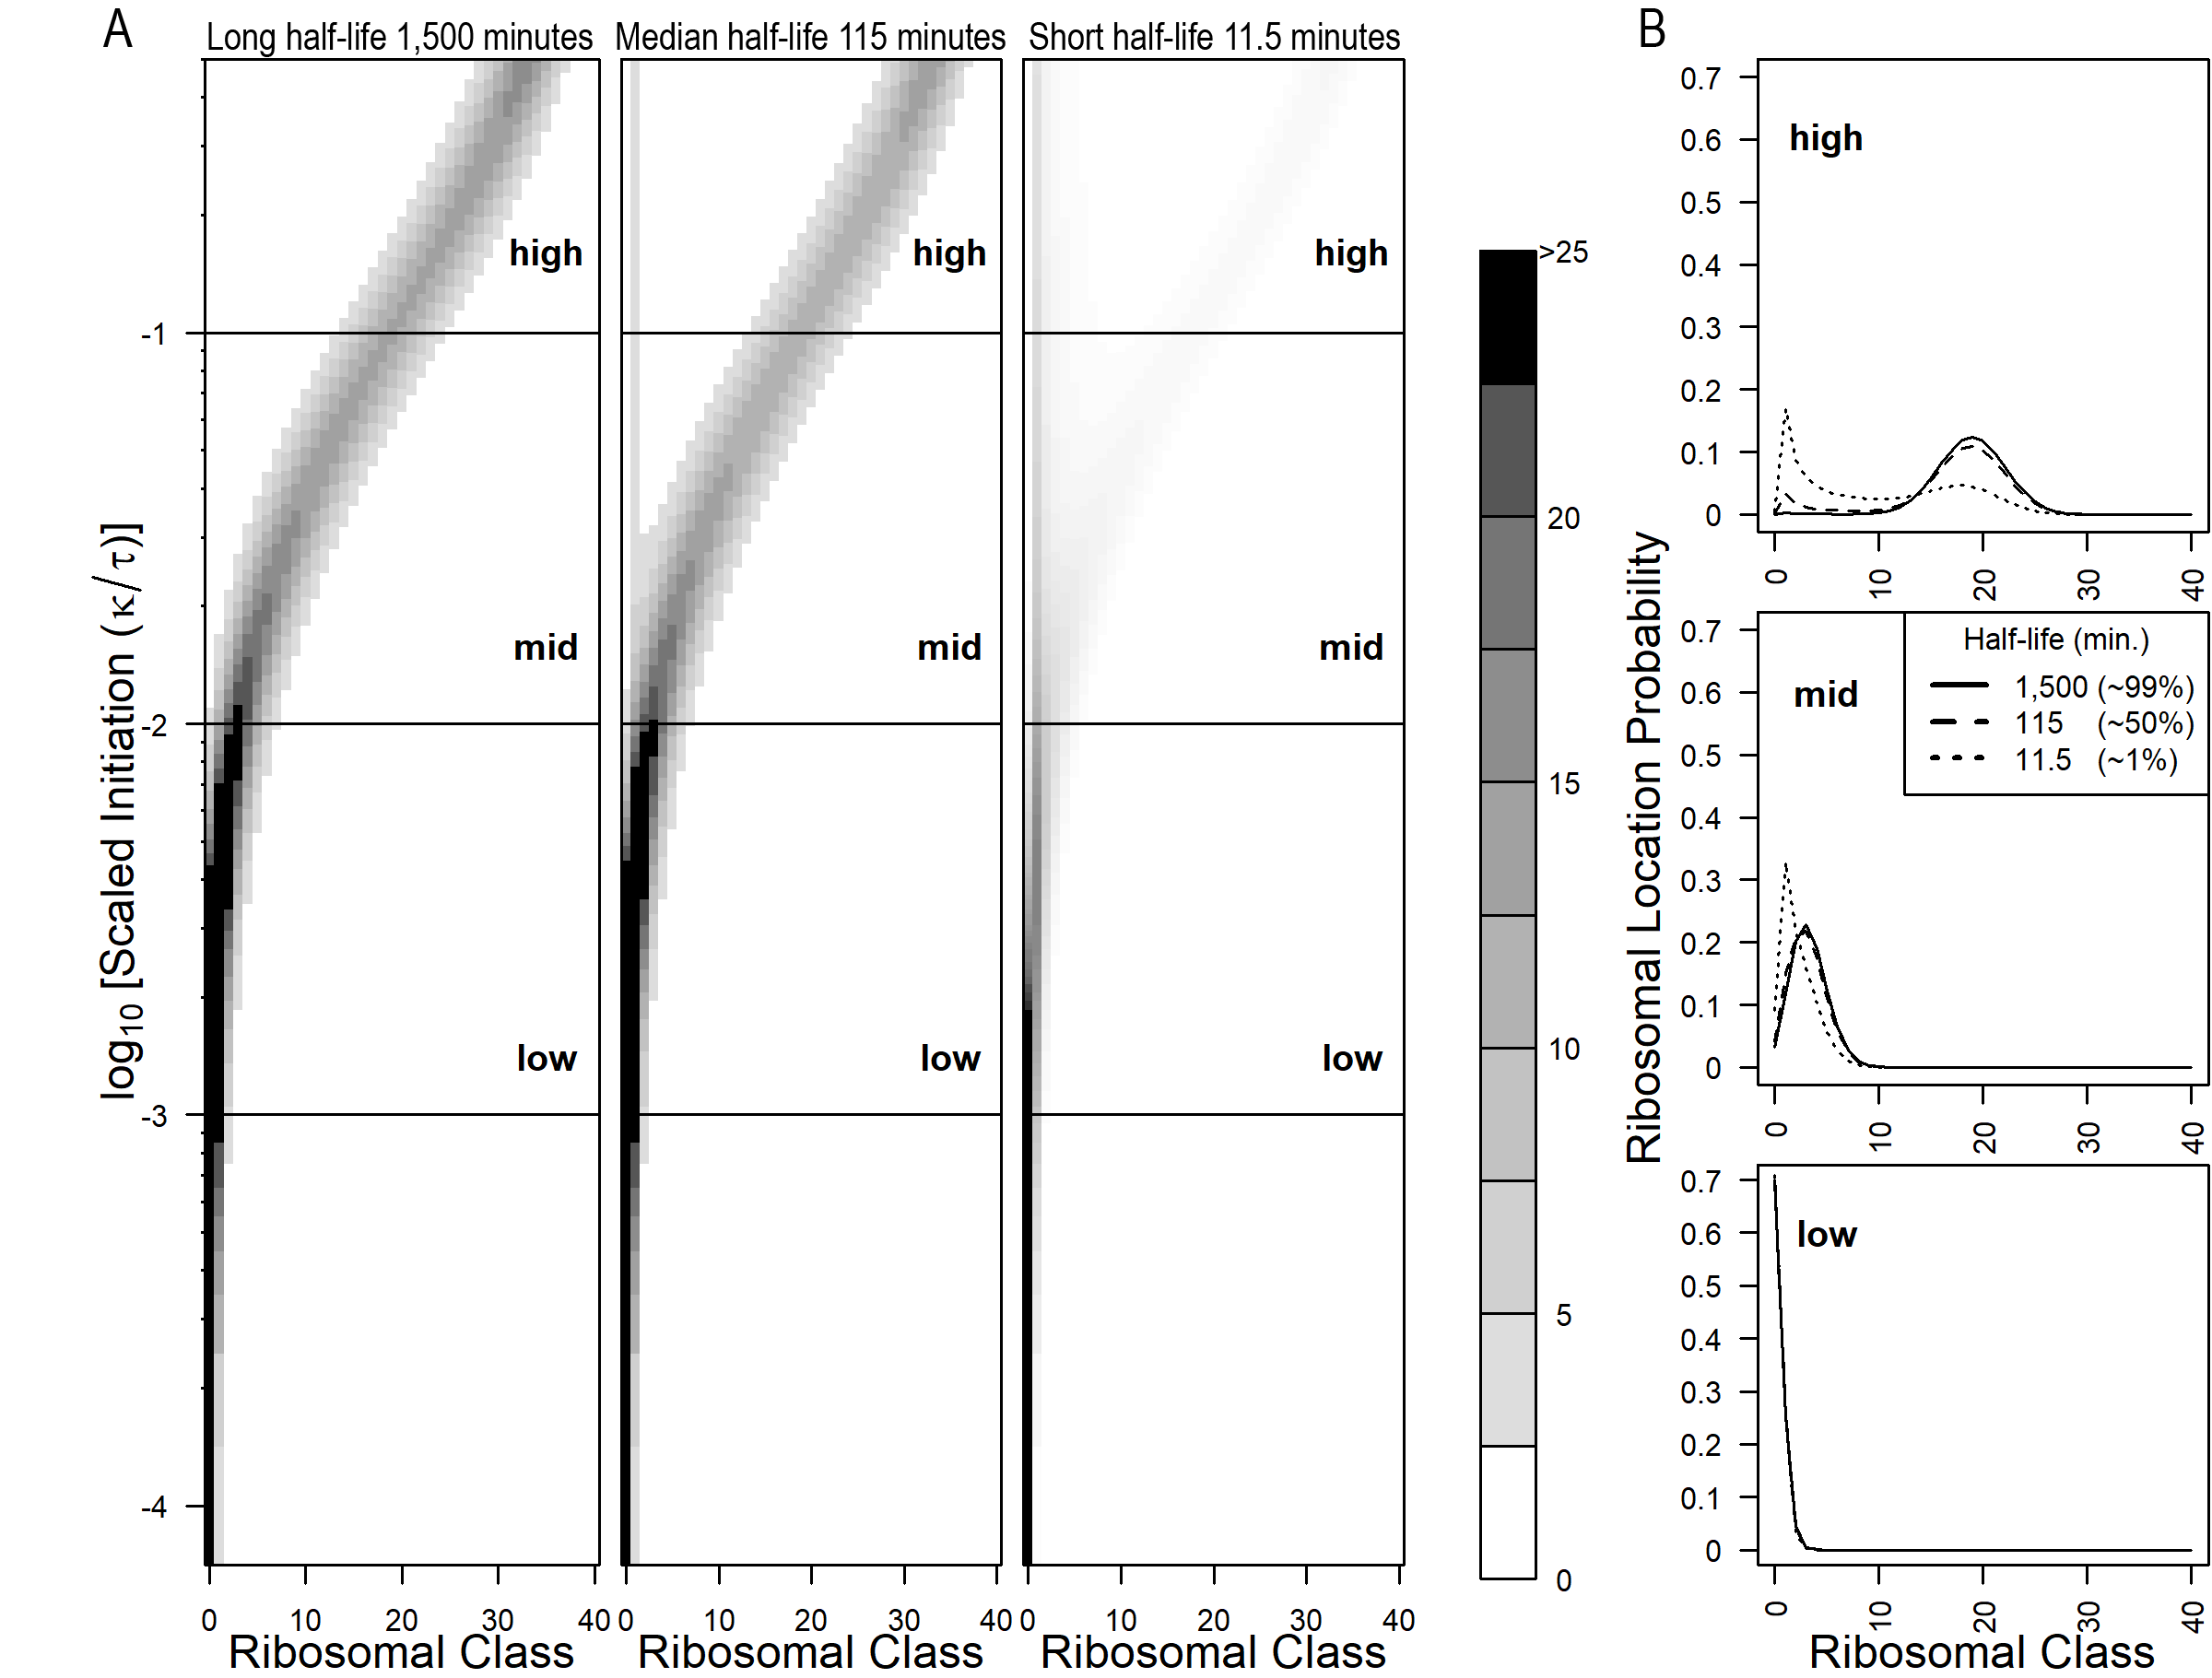
\includegraphics[width=120mm]{Images/2023-07-09_Figure2_At_Marking_Rate_range_medianlength_with_labels.png}
\caption{Low decapping rates $\mu$ in Arabidopsis result in a smaller effect on mRNA distributions in the capped system.  A)  Heatmaps for the full model. Left) low $\mu$ ($7.7\times 10^{-6}$ /s) Center) median $\mu$ (1$\times 10^{-4}$ /s) Right) $\mu$ ($1\times 10^{-3}$ /s) B) individual density profiles for low (0.001), mid (0.01) and high (0.1) scaled initiation values for each $\mu$. All results calculate with \imax = 41.}
%\centering Red: decapped class, Green: capped class, Blue: Total= capped+decapped classes}
\end{figure}
\clearpage



\subsection{decapping rate and ribosomal load determine mRNA distribution between capped and decapped states}
\begin{enumerate}
\item As shown in previous results, higher decapping rates $\mu$ lead to lower MRL in the capped state and increase mRNA abundance in the decapped state.
\begin{enumerate}
  \item Using ~\ref{eq:odds}, we can determine how much of the mRNA population is in the capped state.
  \item We produced output across all scaled initiation values $\kappa'$ and under the 1\textsuperscript{st}, 50\textsuperscript{th} and 99\textsuperscript{th} percentiles for decapping rates in both yeast and Arabidopsis (Figure 8). 
  \item We note two patterns. First as the $\kappa'$ increases, so does the amount of mRNA in the decapped class  \mvechatstar increases. 
  \item Secondly and similarly, higher $\mu$ shifts mRNA population from the capped state to the decapped state as previously seen in Figures 6 and 7.  
\end{enumerate}

\end{enumerate}



%Main results: 
%Link our mean output and the results of TASEP ribosome flow model.
%because short genes experience inteference at short loads becomes accentuated because turnover rate is high
%mention heterologous expression due to codon usage bias
% mean initiation rate to mean elongation rate ratio and shorten it to the Initiation elongation ratio 

%Point for discussion. By varying the granularity of the Ribo flow model it would be possible to fit the model for distinct regulatory regions. In this idea I'm trying to communicate that there might be distinct mRNA regions that behave like different transcripts. Some transcripts might be very granular like every 10 codons has a distinct behavior, But i would imagine that any one major bottleneck in a transcript would make it

\begin{figure}[!ht]
\centering
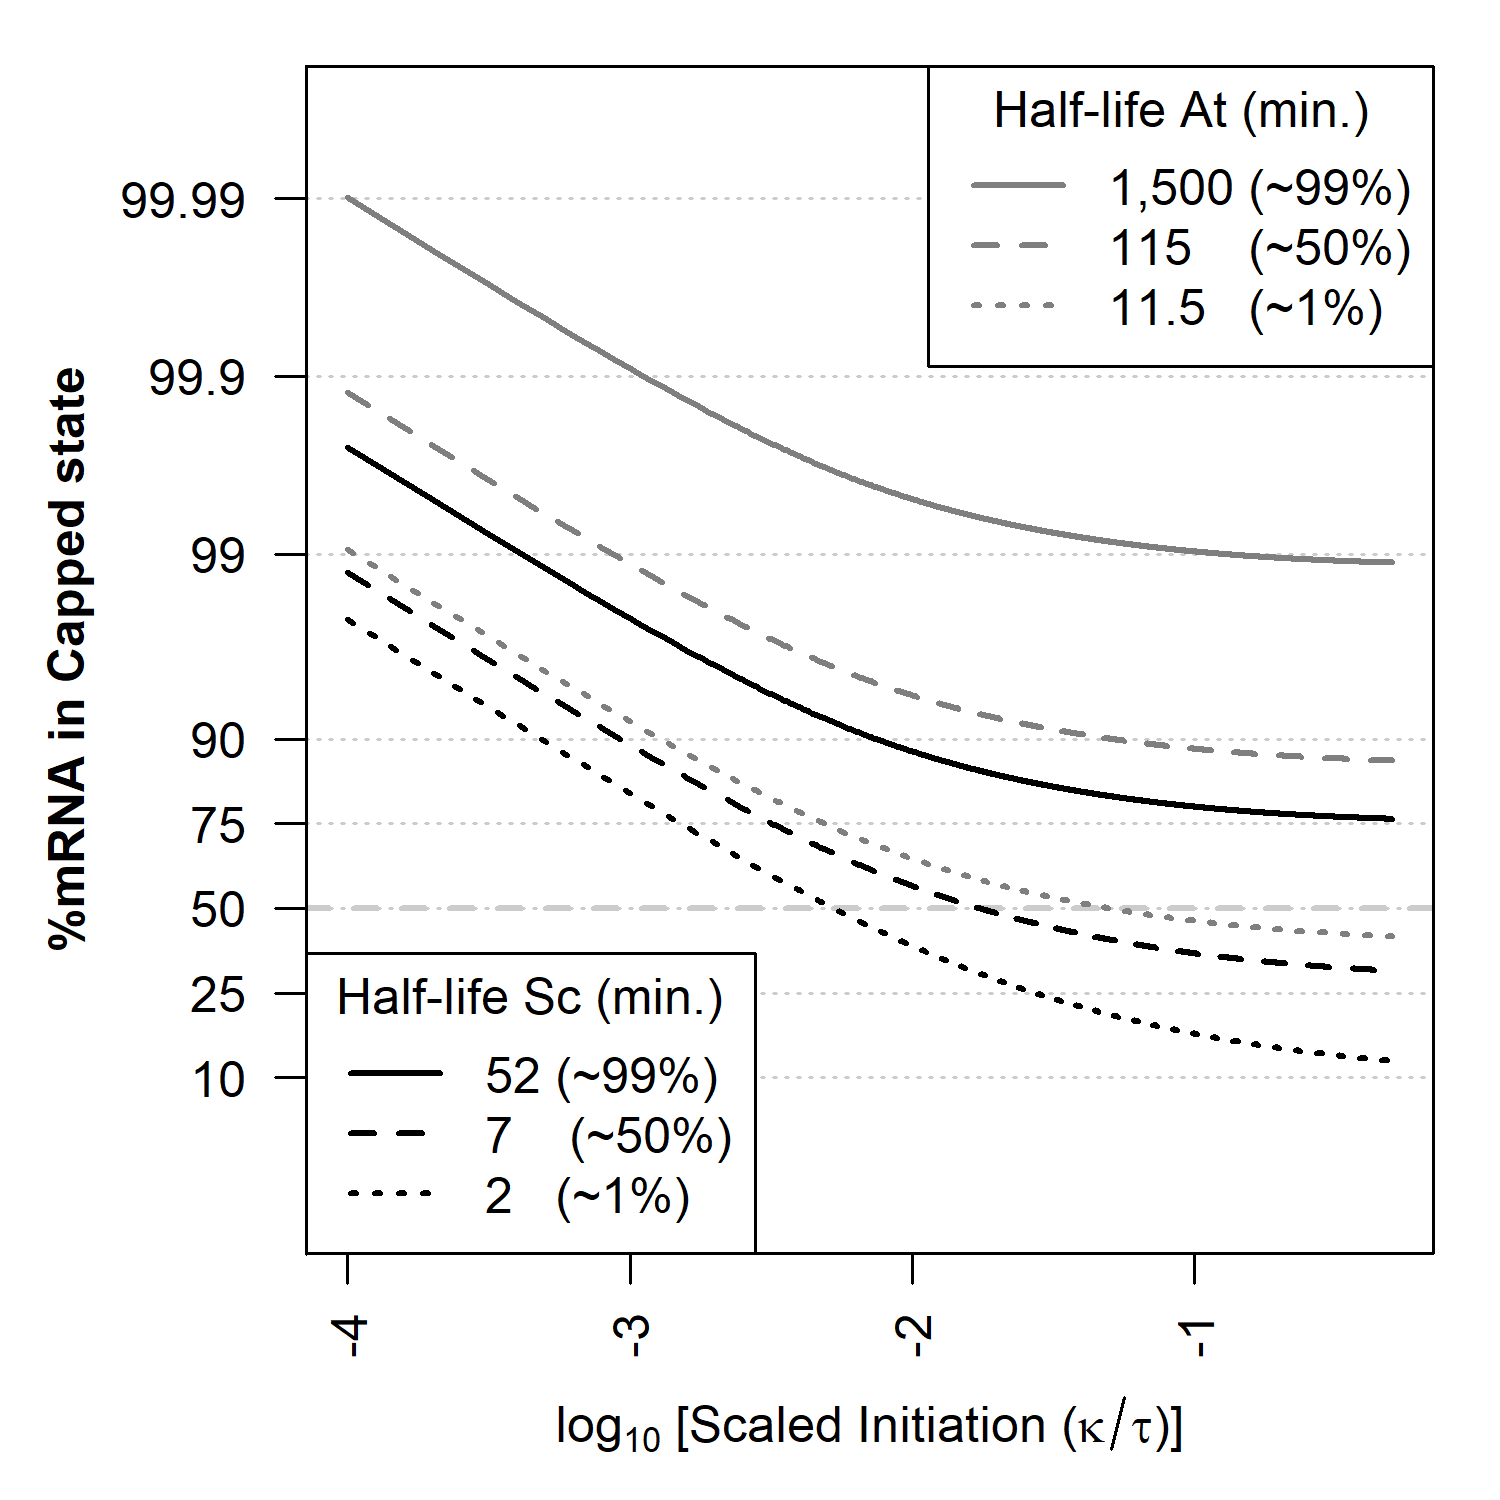
\includegraphics[width=100mm]{Images/2023-07-13_logodds.png}
\caption{Percentage of mRNA in the capped state for a range of decapping rates in yeast ( low $\mu$ ($2\times 10^{-4}$ /s), median $\mu$ ($1.7\times 10^{-3}$ /s), high $\mu$ ($5.7\times 10^{-3}$ /s)) and Arabidopsis( low $\mu$ ($7.7\times 10^{-6}$ /s, median $\mu$ (1$\times 10^{-4}$ /s), high $\mu$ ($1\times 10^{-3}$ /s)). }
%\centering Red: decapped class, Green: capped class, Blue: Total= capped+decapped classes}
\end{figure}
\clearpage

\subsection{At steady state protein production is scales with coding sequence length \imax}
\begin{enumerate}
\item At steady state the MRL increases with coding sequence length and begins to assymptote at high initiation to elongation ratio $\kappa'$ (Figure 9). \rmpar{Mike, you were right. There is a DDI effect on mean ribosomal density. After looking into it deeper I found the old findings completely wrong. Created this new set of results to properly explain the MRL behavior}
\begin{enumerate}
  \item While the capped state MRL is always greater than the decapped MRL, the MRL of the whole system is defined by both capped and decapped MRLs as well as the transcript abundance in each state as shown in eq ~\ref{eq:MRL}.
  \item  As protein length \imax increases, mRNAs enter the decapped state at higher polysome classes. 
  \item Therefore ribosomes take longer  to clear the mRNA, and thus increase the contribution from the decapped state. 
  \item For $\kappa'$= 0.1, the percentage of the mRNA in the capped class is  99\% 78\%  and 35\% for \imax of 4, 39 and 194 respectively.
  \item The \imax dependence is captured in the 1/$\tau$ term in eq ~\ref{eq:odds}, remembering that $\tau = \tau_c/9*\imax$.
  
\end{enumerate}

\end{enumerate}


\begin{figure}[!ht]
\centering
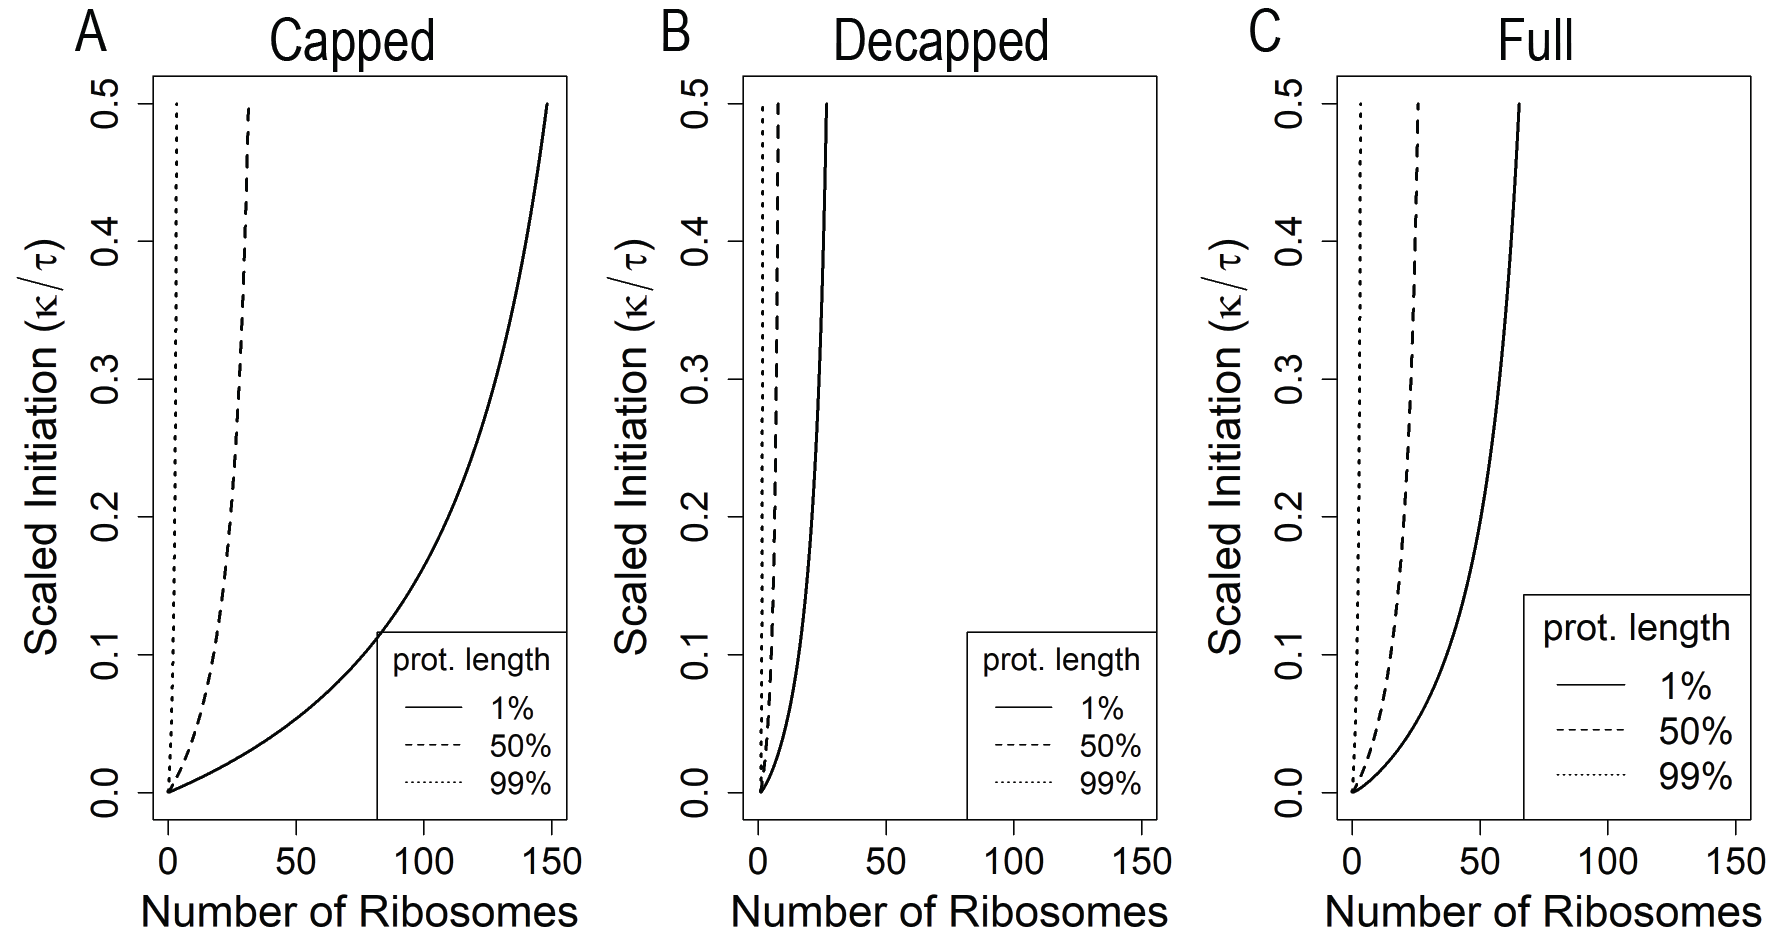
\includegraphics[width=150mm]{Images/MRL.png}
\caption{The mean ribosomal density on a transcript is dependent on coding sequence length. MRL per transcript is higher for longer transcripts. A) Capped state B) Decapped state C) full model. Yeast parameters were used \imax =  4 (1\textsuperscript{st} percentile),  39 (50\textsuperscript{th} percentile), 194 (99\textsuperscript{th} percentile), low decapping rate ($2.2\times 10^{-4}$ /s), over the full scaled initiation range 0.0001- 0.5.}
%\centering Red: decapped class, Green: capped class, Blue: Total= capped+decapped classes}
\end{figure}
\clearpage

\subsection{Decapped state can be a significant source of protein production} \rmpar{may now be superfluous}
%For the capped state rate on is rate off at equilibrium. And by using the initiation rate, it is the same as the protein production rate per transcript. Same applies for %\tau_0$/9*\imax as this is equal to the initiation rate.
%For the decapped state, the equilibrium exists between the inflow of marked transcripts at in a particular distribution and the same %\tau_0$/9*\imax parameter. Or not really. There is really no "on" rate, just an off rate.
%in the capped sytem the on off rate directly relates to the ribosomal density/load on a transcript and it is a decent ad hoc measure of relative expression. 
%Decapped is more complex. The mRNAs enter at rate $\mu$, but these don't carry the same number of ribosomes with them. Unlike $\kappa$ they are not the loading rate of one ribomsome. Is it the mean riboload of the capped system times $\mu$? No, the mean underestimate the contribution of the higher classes needing to percolate down into the lower classes. The decapped class steady state has no simple way of calculating it's steady state load from the parameters.
\begin{enumerate}
\item Protein production rate (PPR) is a function of full model MRL $\times \tau$ and plots normalized to highest protein output are shown in Figure 10.
\begin{enumerate}
  \item As the decapping rate $\mu$ increases it reduces the capped and uncapped MRL as well as shifting transcript abundance to the decapped state (Figure 10A).
  \item  Each of the three cases in Figure 10 A, has been broken down into the PPR contributions from the capped and decapped states (Figure 10 B-D). 
  \item A surprising finding from out model is that when $\mu$ is high ($5.7\times 10^{-3}$ /s), 41\% of all protein production can arise from the decapped state (Figure 10 D).
  \item  The reason behind this is despite the the relative MRL of the decapped state being lower than the capped state as scaled initiation rises, the amount of mRNA in the decapped state rises faster.
\end{enumerate}

\end{enumerate}


 
\begin{figure}[!ht]
\centering
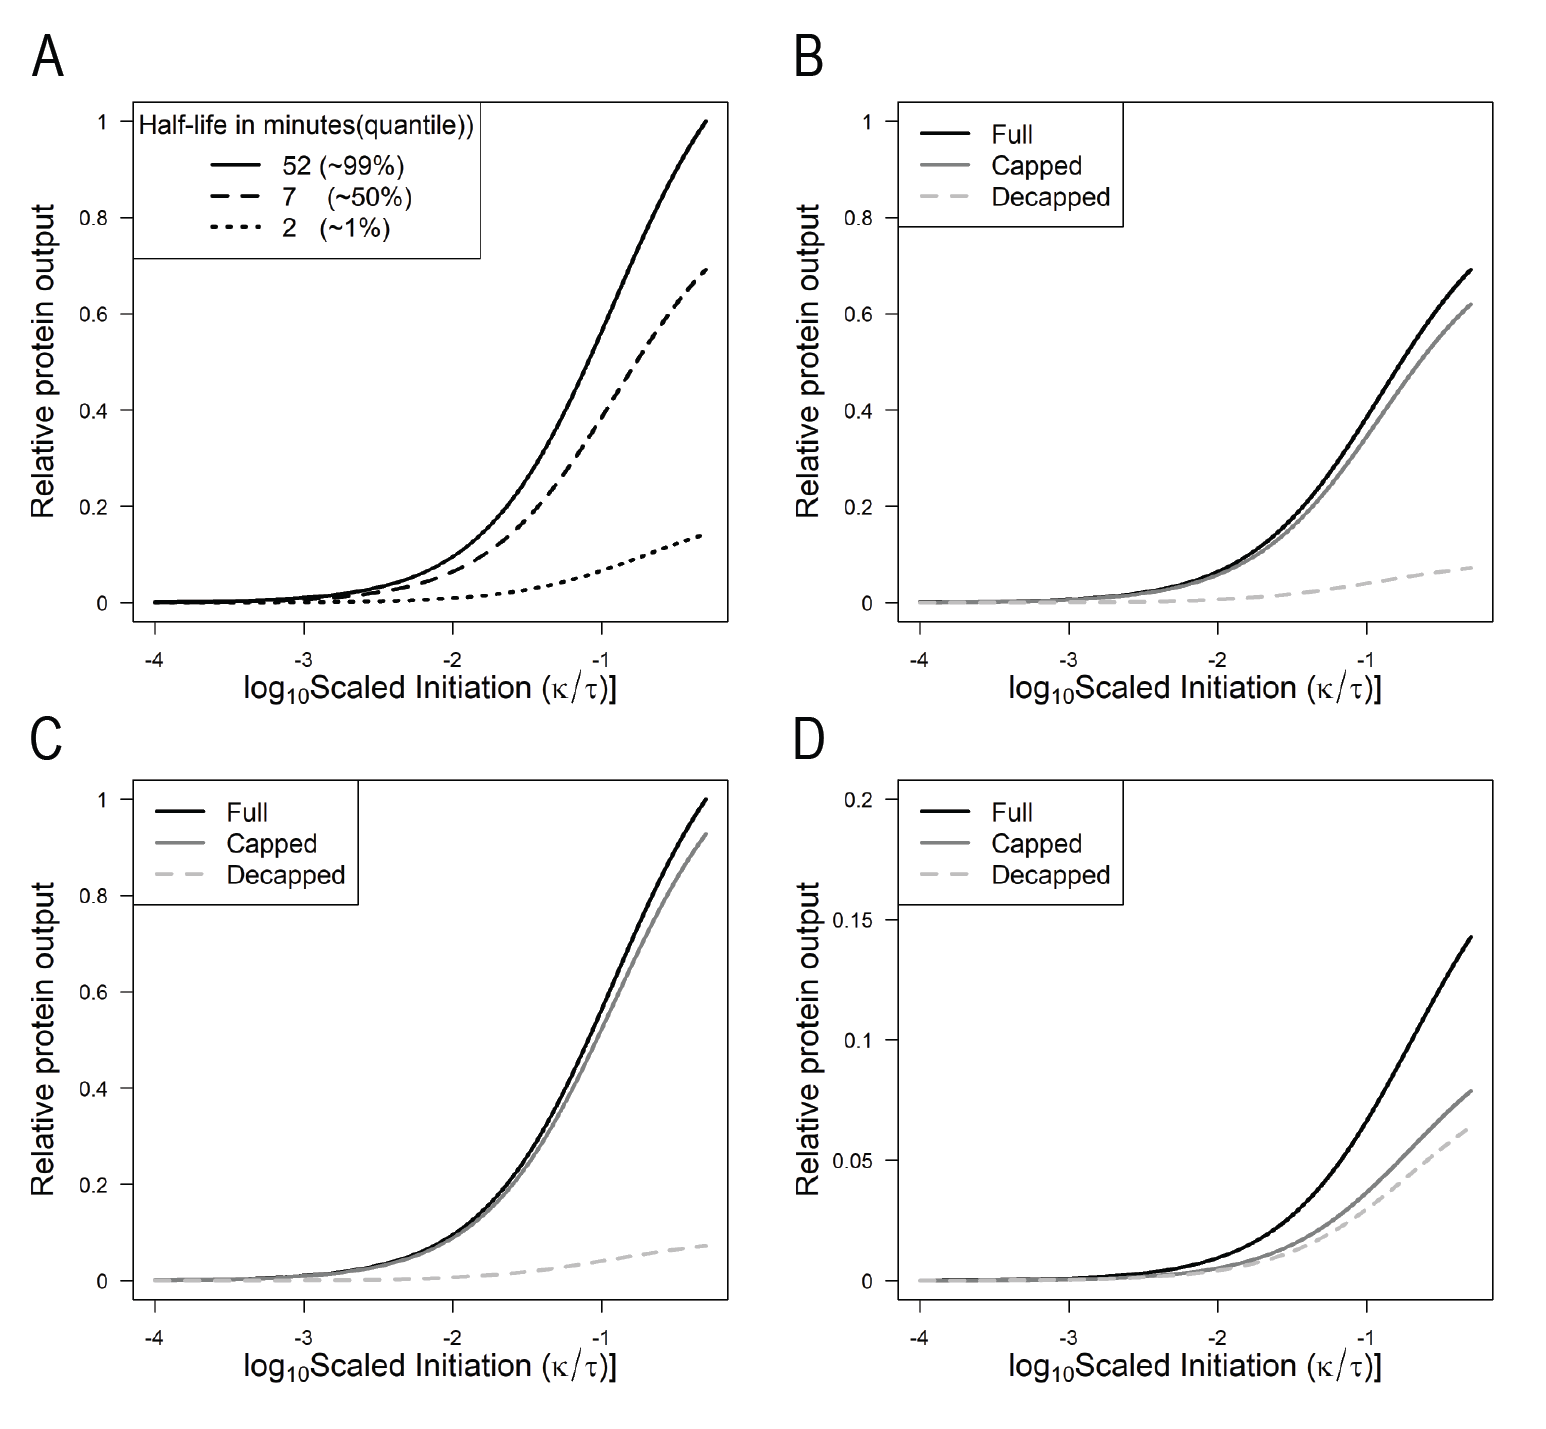
\includegraphics[width = 135mm]{Images/2023-07-17_Protein_Production_v2.png}
\caption{Estimated average protein production in yeast.  A) Protein production across different decapping rates  low $\mu$ ($2.2\times 10^{-4}$ /s), median $\mu$ ($1.7\times 10^{-3}$ /s), high $\mu$ ($5.7\times 10^{-3}$ /s). Total protein production is normalized to the maximal protein production across all parameters. B-D) Contribution of capped and decapped states to total protein production. B) Low decapping C) Medium decapping D) High decapping. }
%\centering Red: decapped class, Green: capped class, Blue: Total= capped+decapped classes}
\end{figure}
\clearpage

\subsection{Model validation}

\begin{enumerate}
\item Gene specific MRL ~\ref{eq:MRL} were calculated for the genes analyzed in Duc and Song 2018 and compared to the empirical MRL calculated from raw data from Weinberg 2016 (Figure 11).
\begin{enumerate}
  \item Model predictions of MRL showed a significant positive correlation to empirical MRLs.
  \item This result is impressive as the model performs well despite no model fitting being performed.
  \item  Model performance is further corroborated with single molecule imaging analyses. Rescaling ribosome abundances from each single molecule study to an \imax of 39 results in loads of 1, 2.4 and 4 ribosomes from (Morisaki 2016), 3 ribosomes (Yan 2016), 4 ribosomes (Wang 2016) and 1.6 (Wu 2016).
%  \item All of which align with low to mid initiation to elongation ratio MRL predictions. 
  %\item Finally, mRNA distributions for the full model agree with signal from polysome traces (Lokdarshi 2020, Dasgupta 2023).
\end{enumerate}

\end{enumerate}


   
\begin{figure}[!ht]
\centering
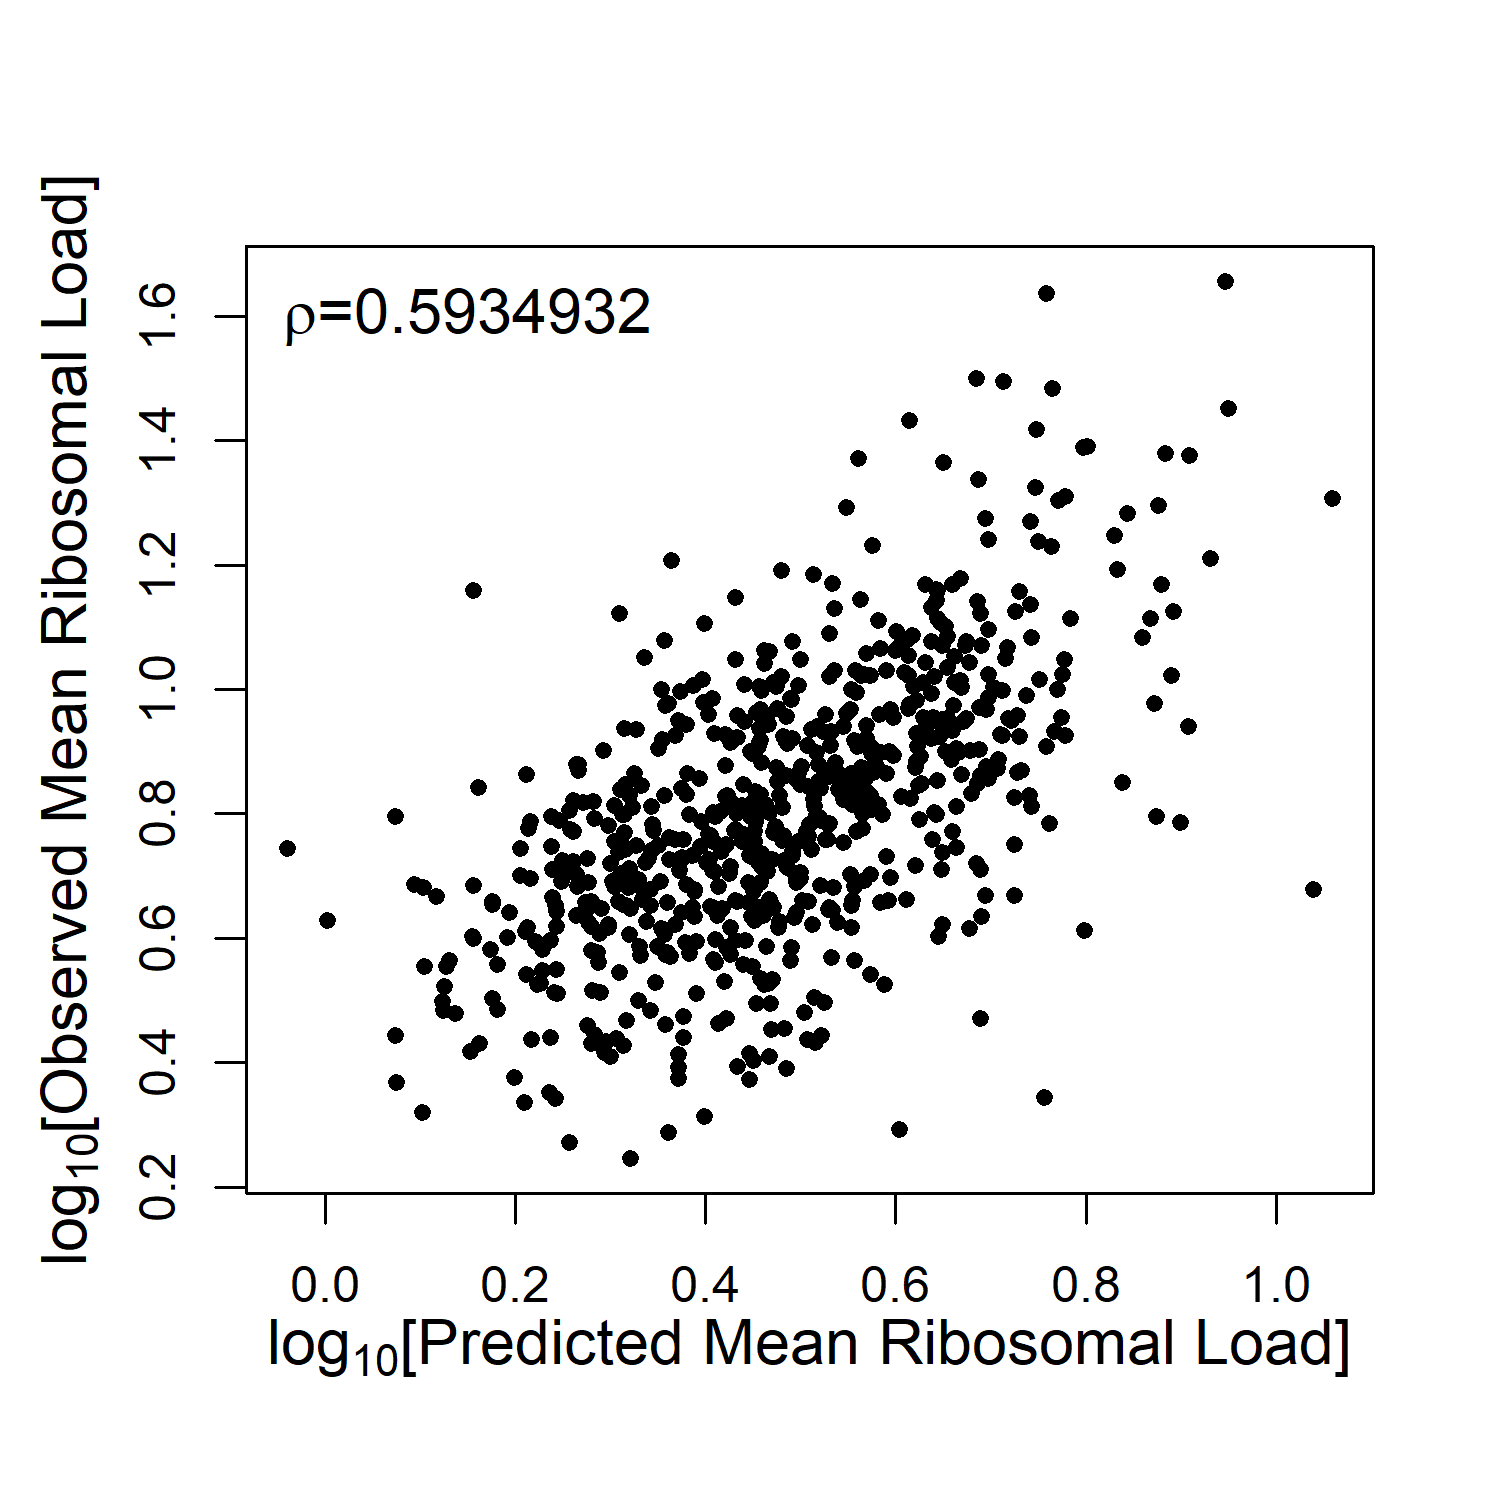
\includegraphics[width=120mm]{Images/Duc_Song_vs_model_log.png}
\caption{Predicted mean ribosomal loads coincide with observed mean ribosomal loads from Weinberg 2016. Using the 850 genes from Duc and song 2018, decapping rates from Presnyak 2015 were mined. Gene specific MRL were calculated and compared to the empircal MRL. Spearman's $\rho$ was calculated and found to be significant, pvalue $<10^{-16}$}
%\centering Red: decapped class, Green: capped class, Blue: Total= capped+decapped classes}
\end{figure}
\clearpage 



\section{Discussion}

In this study we develop, analyze, and validate a novel coupled ODE model of mRNA polysome classes %\mmpar{Terminology: do we like `mRNA polysome populations'?}\rmpar{Yes}
which includes the contributions of mRNA transcription, the initiation, elongation (implicitly), and termination of translation as well as mRNA degradation through 5' decapping and cotranslational decay.
%\rmpar{Need to be specific. \textbf{M:} So be specific.}
%\rmpar{Yes our model is a simplified description of protein synthesis. It contains no new aspects of the process of protein synthesis itself. It does include the interaction between two commonly studied processes. Translation and mRNA degradation. \textbf{M:} So incorporate this fact into the text here or below. Also, isn't the way the model treats ribosomes on the transcripts (uniform as opposed to flux or explicit) novel? \textbf{R:} Done. I don't recall seeing anymodel that treats the ribosomal distribution as uniform. Nor one that looks at it through the length of polysomal classes.}
%\mmpar{(Add relevant equation and figure references to points below)}
\subsection{Model Formulation \& Structure}

Although our model is only a very simplified description of the mRNA polysome population and, in turn, protein translation, it studies the interaction of protein translation with the process of mRNA degradation, a topic which has been underexplored (Yadav 2021). The process of translation is dependent on the underlying population of capped, translationally competent mRNAs. However, empirical measurements suggest that $\sim 12\%$ of transcripts are undergoing co-translational decay (Pelechano 2015). To undergo co-translational decay, the 5' cap has to removed and exonucleases trail behind the last loaded ribosome on a transcript, processing codons as they exit behind the ribosome. 5' decapping is a common pathway in many organisms and accounts for decay for $\sim 68\%$ of Arabadopsis genes (Sorenson 2018).
%  \mmpar{I uncommented this point, can you reconcile it with the previous sentence? \textbf{R:} Done. The first is a statement of the proportion of the population undergoing decay. The second the proportion of the genome that preferentially uses this pathway for decay.} 
Our model includes 5' mRNA decapping followed by cotranslational decay, permiting the analysis of the decapped mRNA state (called degratome in Ma 2020), changes in MRL for capped and decapped states and the contribution of cotranslational decay to protein production.

In addition to being more biologically realistic, structuring the mRNA population by its polysome classes (ribosome load) and the status of its 5' cap allows us to understand how the the rates mRNA production $\lambda$, decapping $\mu$, protein elongation $\tau$, and the clearance rate $\delta$ of decapped and ribosome free mRNAs $\mhatstar_0$ shape the steady state distribution of a gene's mRNA population across polysome classes and capping state (Figures 3-5).
Overall, we find that 


Analytical and numerical solutions show transcription rate $\lambda$ acts as a scaling factor such that the abundances
  % \mmpar{abundance or density? \textbf{R:} Abundance. $\lambda$ scales the density to a number of transcripts. }
  of all of the mRNA polysome classes are proportional to $\lambda$.
  In other words, the total abundance of the capped and decapped mRNA polysome classes $\mvechat$ and $\mvechatstar$ are simply proportional to $\lambda$ (see (\ref{eq:capped_sum}) where $\sum_{i = 0} ^\imax m_i = \lambda/\mu$ and (\ref{eq: marked_total_pop}), respectively).
  The fact that the abundance of the entire capped and decapped mRNA polysome classes are proportional to the transcrption rate $\lambda$ is consistent with intuition, as $\lambda$ increases, so does the abundance of both the capped and decapped populations.
  Similarly, the fact that the abundance of the capped mRNA polysome classes declines as an inverse funcdtion of the decapping rate $\mu$ is also consistent with intuition.
  Because it is the ratio of $\lambda$ and $\mu$, rather than their individual values, that determine the size of the capped mRNA polysome classes, our model indicates that there will be an infinite set of transcription $\lambda$ and decapping rates $\mu$ that can result in the same population size of capped mRNA polysomes.
  All else being equal, this result suggests that these rates could vary greatly between genes with similar abundances.


The fact that changes in the mRNA transcription rate  $\lambda$ only scales, rather than shapes, the relative distribution of mRNA polysome classes allows us to turn our focus to how the remaining model parameters, $\kappaprime = \kappa/\tau, \mu, \text{and} \delta$ alter the \emph{relative} distribution of the capped and decapped mRNA polysome classes \mvechat and \mvechatstar, respectively.

For example, focusing on the relative distribution of the capped mRNA polysome classes $\mvechat$, our model indicates that it is the ratio of scaled translation initiation $\kappaprime = \kappa/\tau$ to decapping $\mu$ which determines the distribution, and thus mean ribosome load, of $\mvechat$  (Figure 3).
   % \mmpar{Starting in the results, let's use \kappaprime to represent $\kappa/\tau$}
    For example, when $\kappaprime/\mu \ll 1$, the distribution of capped mRNA polysome classes $\mvechat$ is greatest in the ribosome free polysome class $i=0$ and declines rapidly with with ribosome load $i$.
    As $\kappaprime/\mu$ increases, the distribution of capped mRNA polysome classes shifts away from the lower bound of $i = 0$ appears to follow a truncated gaussian distribution.
    In contrast, it is only at very high and generally unrealistic values of $\kappaprime/\mu$ (i.e. $\kappaprime/\mu > 10$) do we see the peak of the distribution of capped mRNA polysome classes approach $\imax$.
 %   \mmpar{Is my revision correct? \textbf{R:} yes}



Shifting our focus to the relative distribution of the decapped mRNA polysome classes \mvechatstar, our model provides a number of important insights .
Surprisingly, in the special case of the decapped, ribosome free mRNA class $\mhat_0^*$, we find its abundance is decoupled from the dynamics of the rest of the population.
  This decoupling has a number of important implications.
  For example, the steady state abundance of $\mhat_0^* = \lambda/\delta$ and, thus, depends only on the ratio of the mRNA transcription rate $\lambda$ to the mRNA clearance rate $\delta$ (equation \ref{eq:decapped_solution}).
  If the transcription rate $\lambda$ of new, capped, but ribosome free mRNAs $\mhat_0$ is substantially lower than the per capita mRNA clearance rate of decapped, ribosome free mRNAs $\delta$, such that  $\lambda \ll \delta$, then our model predicts that there will be few mRNAs in the $\mhat_0^*$ class $\mhat_0^* \ll 1$.
  Because $\mhat^*_0$ has no impact on the rest of the mRNA population, this result allows us to greatly simplify our analysis since we need not consider $\mhat_0^*$ nor the parameter $\delta$.

Focusing now on the steady state abundance of the ribosome occupied decapped mRNA polysome classes, i.e.  $\mhat_i^*$ where $i > 0$, we find that the distribtuion of $\mhat^*_i$  depends on the gene specific ribosome elongation rate $\tau_0$ (where `elongation`  includes the ribosome's reading of the mRNA's stop codon) and the distribution of capped mRNA $\mhat_i$ with $i > 0$ (Figure 4).
\label{item:protein_production} This finding implies that because the density of $\mhat^*_i$ monotonically decreases with $i$, the distribution of decapped mRNA polysome classes is skewed and dominated by lower polysomal classes.
  This is monotonic decline coupled with the fact that the decapped ribosome free polysome class $\mhat_0$ does not contribute to protein production, implies that MRL of the decapped mRNA polysomes is must be less than MRL the of the capped mRNA polysomes.
  Thus, while the decapped class does contribute to protein production, substantially under particular parameter values ($\mu> 5.7 \times 10^{-3}$ or $\imax >> median \imax$), its contributution to the mRNA population's protein production will always be less than  $50\%$.



The full model combines the distributions of the capped and decapped states and is equivalent to mRNA population that is often measured in translational assays.
The full model distribution is strictly unimodal when the majority of trasncripts are in the capped state ($\sum \mvechat >> \sum \mvechatstar$), effectively when $\kappaprime/\mu \ll 1$ (Figure 6 and 7).
The distribution is also unimodal when the $\kappaprime << 0.01$, meaning that the MRL is low and near the $i=0$ bound. 
In all other cases the distribution is bimodal. The high MRL peak arises from the capped state, while the small MRL peak comes from the decapped states. 

The model formalizes the interplay between mRNA decapping $\mu$ and initiation elongation ratio $\kappa/\tau$ and its effect on protein production.
By multiplying the state specific MRL [\ref{eq:MRL}] by $\tau$ we can estimate protein production rate.
Shifts in mRNA between capped and decapped states as well as changes in MRL control protein production.
As expected, increasing $\mu$ raises the proportion of decapped transcripts \mvechatstar compared to capped transcripts \mvechat.
Increasing ratio of initiation to elongation rates $\kappa/\tau$ also results in an increase of decapped mRNAs \mvechatstar.
As $\kappa/\tau$ increases the MRL of the capped population \mvechat increases, transcripts enter the decapped state at higher polysomal classes and thus take longer to reach $m_0^*$.
At high $\mu$ this shift in transcripts is enough to partly overcome the fact that the decapped MRL $\leq$ the capped MRL.
One final consideration is the assumption that the mRNA clearance rate $\delta >> \lambda$, and therefore $\mhatstar_0$ will be negligible. If $\mhatstar_0$ is small our current results act as an upper bound of the protein production contribution from the decapped class. 


A unique property of our model is that it can differentiate the capped and decapped states individual contributions to protein production. 
A surprising prediction from our model is that genes with  high decapping rates (e.g. $\mu  \sim 5 \times 10^{-3}$ or a half-life of $\sim 120 \sec$) has almost (but never more than) half of its protein production coming from the decapped mRNA polysome classes (Figure 10).
The high protein production from the decapped state suggests that high decapping rate transcripts can produce more protein than would be expected from their capped MRL alone. 


\subsection{Model Validation}

In addition to studying the general behavior of our model, we validate this behavior using empirically based parameter values from the literature.
In general, we find that our model's predictions of mRNA distributions, when parametrized with biologically relevant values, are highly consistent with a wide range of empirical data.
For example, we predicted MRL using empirical values for initiation elongation ratio $\kappa'$ (Duc and Song 2018) and decapping rate $\mu$ (Presnyak 2015) and compared them to the empirical MRL from (Weinberg 2016) and found a strong correlation despite having performed no fitting. This supports the idea that the model is a useful representation of the complex processes underlying protein production.
The $\kappa'$ estimates utilized are only for highly translated genes (16\% of alll detected genes), and most others would fall in a range of $\kappa'<0.01$ (Duc and Song 2018).
Taking the overall low $\kappa'$ values, our model predicts that a median length protein of \imax =39 (351aa) would have 10 or fewer ribosomes loaded, which agree with the predominance of low polysomes (<10) seen polysome gradient traces (Lokdarshi 2020, Dasgupta 2023). 
By the same logic, we find that single molecule measurements of translation (Morisaki 2016, Yan 2016, Wang 2016, Wu 2016, Section 3.6) all fall in the same low polysome range.
Finally, the fraction of mRNA predicted in the capped and decapped class  are consistent with population wide estimates (Pelechano 2015, Figure 10). 


\subsection{Model limitations, extensions and future work}

Our model's assumptions about the process of mRNA decapping, the continued competence of ribosomes present prior to decapping, and degradation of mRNA solely from the decapped and ribosome free class $m_0^*$  closely resembles the biological process of co-translational mRNA decay. While the existence of co-translational mRNA decay is well established (Sorenson 2018, Pelechano 2015), other mechanisms exist with different outcomes for translation. 3' decay results in no ribosomes terminating and would send all transcripts into the $m_0^*$ class . Mechanisms utilizing endonucleolytic decay due to no go decay or nonsense mediated decay would potentially allow ribosomes downstream of the cleavage site to terminate but not those upstream (Urquidi-Camacho 2020, Merchante 2017). Thus, depending on the ditribution of mRNAs in the capped class, and the site of the endonucleolytic decay a transcript in $m_i$ would end up in $m_{j}$, where $j < i$.
Developing a more quantitative understanding of how different factors affect a gene's mRNA stability and, in turn, protein expression, relevant to a wide range of applied molecular biology (e.g. the design of efficient heterologous genes expression and mRNA vaccines) (Cheng 2023 viruses, Boo and Kim 2020).

Current debate is focused on the contributions of the protective effects of ribosome association vs. ribosome stalling to mRNA transcript stability.
While our model currently does not include the protective effects of translation or stall prone codons, it should be possible to do so.
The protective effects of ribosomal loading which could be modeled by making the decapping rate $\mu $ by $(1-i/\imax)$, or having one, higher decapping rate for $m_0$ and a lower decapping rate for the other polysomal classes.
The protective effects of translation could increase per ribosome, but eventually at high MRL could trigger ribosome associated decay pathways through ribosomal collisions. This would require analysis on an individual transcript basis.
Our model does not consider codon specific effects such as pausing sites, difficult to fold regions of a protein or codon optimality, or protein quality control (Wu and Bazzini 2023).
Pausing sites could be addressed by splitting each polysome class into two regions and could approximate a ribosome flow model of only two regions, a 5' and 3', split by the pausing site. Current models of translation focus mainly on the behavior of the average transcripts. However this ignores th



%
%
%
%
%
%
%
%
%
%
%
%
%
%
%
%\begin{enumerate}
%\item Summary paragraph of results?
%
%
%\item mRNA decay not only regulates transcript abundance, but also reduces mean ribosomal load.
%	\begin{enumerate}
%		\item This reduction can be interpreted as a inhibiting the system from reaching the unobstructed steady state. This has previously been suggested but not demonstrated by (Reuveni 2011) and explored by (Valleriani 2011). 
%		\item This suggests that if left given enough time in the capped state each transcript species would reach a characteristic MRL during a set period of time.
%		\item  
%
%	\end{enumerate}
%	\begin{enumerate}
%	\item	Points for results
%
%	\end{enumerate}
%
%\item In addition to the effects on the distribution of transcripts across polysomal classes, decapping rate along with the scaled translation initiation rate determine the distribution of mRNA across the two states. 
%	\begin{enumerate}	
%		\item Mature mRNA populations and their degradation has been modeled before, but in absence of translation and it's quality control effects (Cao and Parker 2001, Cao and Parker 2003, Wu 2013, Wu 2016, Zupanic 2016, reviewed in Ashworth 2019). 
%		\item Our model shows that even decapped populations of mRNAs can produce protein and can be the most abundant species of mRNA in the population. 
%		\item Through 5'P mRNA sequencing Pelechano 2015 can track degradation intermediates. They find that degradation products in the CDS follow a 3 nucleotide periodic pattern and compose 12.4 of all reads recovered. This indicates that a significant portion of the bulk mRNA population is undergoing cotranslational decay.
%		\item  Figure 9 shows that a significant amount of mRNA can be found in the decapped state.
%Most transcripts will have a scaled translation initiation rate below 0.01 and have most of the mRNA in the capped state. However, our model result is on a per gene basis. To estimate a the global proportion of decapped to capped mRNA will require a larger sample of marking, transcription and scaled translation initiation rates.
%	\end{enumerate}
%	\begin{enumerate}
%	\item	Points for results
%	\item mention pelechano in results briefly
%	\end{enumerate}
%
%
%\item	Co-translational decay may allow for decapped transcripts to provide substantial protein production.
%	\begin{enumerate}
%	\item A surprising result from our model is that genes with short half-lives can have almost half of their protein produced in the decapped state. 
%	\item This suggests that short lived transcripts can produce more protein than expected despite having a half-life comparable to the time it takes an average length protein to get translated.
%	
%	\end{enumerate}
%	\begin{enumerate}
%	\item	Points for results
%
%	\end{enumerate}
%
%
%\item	Model Limitations, extension and future work, modeling decay
%	\begin{enumerate}
%	\item The 5' mRNA decay pathway presented in our model most closely resembles that of co-translational decay, and in Arabidopisis 68\% of mRNAs are degraded this way (Sorenson 2018).
%		\item However, other mechanisms exist with different outcomes for translation. 3' decay would result in no ribosome terminating and abruptly remove a subset of transcripts and overall protein production from the pool. Endonucleolytic decay due to NGD or NMD would potentially allow ribosomes downstream to terminate but not those upstream (Urquidi-Camacho 2020, Merchante 2017).
%		\item Extension of the model to include these mechanisms is yet to be explored. However, it is safe to speculate that they would both result in a further reduction of MRL.
%		\item Our model also used two conservative set of decapping rate estimates (Presnyak 2015 and Sorenson 2018). 
%	
%	\end{enumerate}
%	\begin{enumerate}
%	\item	Points for results
%
%	\end{enumerate}
%
%\item	Model extension and future work, Codon opt
%	\begin{enumerate}
%	\item Currently there is a debate whether mRNA stability is regulated primarily through the protective effects of ribosomal association or through the suboptimal codons causing ribosomal stalling and the subsequect ribosome associated decay pathways  (Chan 2018 elife).
%	\item Our model currently cannot distinguish between the protective effects of translation, codon effects or other decay pathways.
%	\item In the current implementation of the model we did not directly explore the protective effects of ribosomal loading. This could be first implemented by including a similar weighting term analogous to the wieght for the intiation rate of (1-i/\imax).
%	\item Our model does not consider codon specific effects such as pausing sites. 
%	\item Difficult to fold or translate regions of a transcript  could be further modeled by splitting each transcript species into two or three regions defined biologically by pausing sites. This would resemble a nested ribosome flow model withing our model structure. 
%	\item These hyptotheses could be tested by fitting out model to the Chan 2018 dataset.
%	\item The protective effects of translation could increase per ribosome, but eventually at high loads  could trigger ribosome associated decay pathways through ribosomal collisions. This would require analysis on an individual transcript basis.
%	\end{enumerate}
%
%\item Model Extension: Population level modeling with degradation
%	\begin{enumerate}
%	\item Modeling individual transcripts is of value to understand the mechanism of translation.
%	\item Our model does not account for limitations in the tRNA or ribosome pools.
%	\item Modeling of the all the species of transcript (Nanikashvili 2019, Raveh 2016) and taking to account ribsome availability have been done previously (Shah 2013), but without considering mRNA degradation.
%	\item Our model is extensible to modeling the full mRNA population of a sample.
%	\end{enumerate}	
%	\begin{enumerate}
%	\item	Points for results
%
%	\end{enumerate}
%
%\end{enumerate}
%
%
%
%
%
%
%
%\begin{enumerate}
%\item In this work we present a model which tracks mRNA populations and their association with ribosomes across two states, a translationally competent capped state and incompetent decapped state. 
%	\begin{enumerate}
%	\item As the process of translation is entirely dependent on its mRNA substrate to produce protein, understanding the underlying fluctuation in mRNA is crucial. 
%	\item We demonstrate that the process of marking an mRNA for degradation through decapping alters the total number of mRNA molecules in a system, their distribution between the two states as well as lowering the mean number of ribosomes on a transcript. 
%	\item A surprising outcome of this process is that, under certain biological conditions, a substantial amount of protein produced may arise from terminating ribosomes in the decapped state.
%	\end{enumerate}
%\end{enumerate}
%
%\begin{enumerate}
%\item The model recapitulates empirical measurements of translation.
%	\begin{enumerate}	
%	\item Despite the model itself not being fit to data, through use of empirically obtained parameter values it still displays ribosomal loading patterns that would be expected in polysome profiles. 
%	\item In polysome profiles all transcripts in a sample are separated based on the number of ribosomes translating on them.
%	\item The majority of transcripts are found with 1-10 ribosomes and strongly bias towards lower ribosomal loads (Weinberg 2016, Lokdarshi 2020).
%	\item Throughout the scaled translation initiation range we observe that, for a protein of average length and transcripts with a long half-life, the transcript is below a MRL of 10 for the majority of the range. 
%	\item Moreover, Duc and Song 2018, only studied the most highly translated genes (850 out of 5,300 expressed genes). This means that a majority of translated genes fall below the scaled translation initiation range used in this study.  
%%morisaki uses 10xFLAG-TAG which they call spaghetti monster. Flag tag is 8aa long. so 80aa tag. Plus 1544aa long KDM5B, or 374aa long beta actin or 125aa long H2B. The average ribosomal load estimated was 5, 3 and 2.2 respectively. Converting them to \imax that would be (80+1544)/9= 180,(80+374)/9=  50 and (80+125)/9= 22. and the densities would be 0.0277, 0.06, and 0.1. Converting to model \imax of 40, 1.1118, 2.4 and 4 ribosomes each. 
%%Yan uses a 24xSunTag kif18b PP7 reporter. only the suntag and kif are protein coding. A suntag has a length of 24 aa and kif18b 852aa. so total length is 852 + 24*24 = 1482. \imax of 158. the relative frequency of mRNAs with ribosomes are an average of 12 with a range of 1 to 30.  that is a density of 0.076 +- 0.0063 to 0.19. in \imax 40 that is 3 +- 0.25 to 7.6. 
%%Wang also uses a 24x suntag, but with ODC (461aa) as the protein. 461+24*24= 1037. \imax = 115. with an average ribosomal load of 12 +- 1-37. density of 0.104 +- 0.009 to 0.322. in \imax 40 that is 4.16 +- 0.36 to 13
%%Finally wu usese a 1x flag 24xsuntag blue fluorescent protein (239) and an auxin induced degron (228). total length is 1051. \imax is 116. mean of 5. 0.043 and at \imax 40 1.7.shorter and longer constructs allowed wu to see that number of ribsomes linearly scale with construct length .  agreeing with our results and indicating that their estimates are very likely steady state estimates.
%
%	\item This is further corroborated with single molecule imaging analyses. Rescaling ribosome abundances from each study to an \imax of 40 results in loads of 1, 2.4 and 4 ribosomes from (Morisaki 2016), 3 ribosomes (Yan 2016), 4 ribosomes (Wang 2016) and 1.6 (Wu 2016). 
%	\item Wu 2016, also designed constructs containing different lengths of protein sequences and found that ribosome load scales linearly with protein length. Agreeing with our results in Figure 8 and implying the measurement was performed at true steady state. 
%	\item Despite this general agreement, the model still represents an upper bound of translation as many other forms of translational control are not included. 
%	\end{enumerate}
%\end{enumerate}
%
%\begin{enumerate}
%	\item Our model integrates the effect of mRNA decay into translation.
%	\begin{enumerate} 
%		\item mRNA decay not only regulates transcript abundance, but also reduces mean ribosomal load.
%		\item This reduction can be interpreted as a inhibiting the system from reaching the unobstructed steady state. This has previously been suggested but not demonstrated by (Reuveni 2011) and explored by (Valleriani 2011). 
%		\item This suggests that if left unobstructed each transcript species would reach a characteristic MRL during a set period of time. 
%		\item The 5' mRNA decay pathway presented in our model most closely resembles that of co-translational decay, and in Arabidopisis 68\% of mRNAs are degraded this way (Sorenson 2018).
%		\item However, other mechanisms exist with different outcomes for translation. 3' decay would result in no ribosome terminating and abruptly remove a subset of transcripts and overall protein production from the pool. Endonucleolytic decay due to NGD or NMD would potentially allow ribosomes downstream to terminate but not those upstream (Urquidi-Camacho 2020, Merchante 2017).
%		\item Extension of the model to include these mechanisms is yet to be explored. However, it is safe to speculate that they would both result in a further reduction of MRL.
%		\item Our model also used two conservative set of decapping rate estimates (Presnyak 2015 and Sorenson 2018). 
%	\item Currently there is a debate whether mRNA stability is regulated primarily through the protective effects of ribosomal association or through the suboptimal codons causing ribosomal stalling and the subsequect ribosome associated decay pathways  (Chan 2018 elife).
%	\item Our model currently cannot distinguish between the protective effects of translation or 
%	\item In the current implementation of the model we did not directly explore the protective effects of ribosomal loading. This could be first implemented by including a similar weighting term analogous to the wieght for the intiation rate of (1-i/\imax).
%	\item However, biology suggests a more complex behavior.
%	\item The protective effects of translation could increase per ribosome, but eventually at high loads  could trigger ribosome associated decay pathways through ribosomal collisions. This leaves much to be explored further	
%	\end{enumerate}
%\end{enumerate}
%
%
%\begin{enumerate}
%	\item In addition to the effects on the distribution of transcripts across polysomal classes, decapping rate along with the scaled translation initiation rate determine the distribution of mRNA across the two states. 
%	\begin{enumerate}	
%		\item Mature mRNA populations and their degradation has been modeled before, but in absence of translation and it's quality control effects (Cao and Parker 2001, Cao and Parker 2003, Wu 2013, Wu 2016, Zupanic 2016, reviewed in Ashworth 2019). 
%		\item Our model shows that even decapped populations of mRNAs can produce protein and can be the most abundant species of mRNA in the population. 
%		\item Through 5'P mRNA sequencing Pelechano 2015 can track degradation intermediates. They find that degradation products in the CDS follow a 3 nucleotide periodic pattern and compose 12.4 of all reads recovered. This indicates that a significant portion of the bulk mRNA population is undergoing cotranslational decay.
%		\item  Figure 9 shows that a significant amount of mRNA can be found in the decapped state.
%Most transcripts will have a scaled translation initiation rate below 0.01 and have most of the mRNA in the capped state. However, our model result is on a per gene basis. To estimate a the global proportion of decapped to capped mRNA will require a larger sample of marking, transcription and scaled translation initiation rates.
%	\end{enumerate}
%\end{enumerate}
%
%\begin{enumerate}
%	\item Co-translational decay may allow for decapped transcripts to provide substantial protein production. 	
%	\begin{enumerate}
%		\item A surprising result from our model is that genes with short half-lives can have almost half of their protein produced in the decapped state. 
%		\item This suggests that short lived transcripts can produce more protein than expected despite having a half-life comparable to the time it takes an average length protein to get translated.
%	\end{enumerate}
%		\item We also highlight that all examples in the model have been run under the same transcription rate $\lambda$. The underlying amount of transcript will scale protein output globally, which translation and mRNA degradation will subsequently tune.
%	\begin{enumerate}
%		\item We have not correlated protein production to transcription as in (de Sousa Abreu 2013, Schwanhauser 2013, Edfors 2016, Brion 2020) due to not modeling protein degradation. 
%		\item Properly setting the transcription rate is important for determining final protein production, but not for understanding the translational dynamics.
%	\end{enumerate}
%\item In our model the remaining transcripts in class $m_0^*$ are either only the 3' end of co-translationally degraded transcripts or full transcripts from class $m_0$.
%	\begin{enumerate}
%		\item The role of the degradation rate  is to account for the remaining transcripts.
%		\item Mathematically and biologically it is essential for completing the lifecyle of an mRNA, but difficult to measure.
%	\end{enumerate}
%\end{enumerate}
%
%\begin{enumerate}
%	\item The model suggest that regulation mechanisms for translation are concerned with reducing MRL.
%	\begin{enumerate}	
%		\item This is first seen by comparing DII, the simplest, most unobstructed model to the DDI model. 
%		\item As scaled translation initiation rates increase, density dependence reduces MRL. We do not include bottlenecking due to translational folding, codon optimality or pausing in our model therefor density dependent effects might occur earlier in a transcript. 
%		\item With in the design of our model this would mean a transcript would behave as if its total length were <\imax. Given a shorter effective \imax for translation.
%		\item This particular aspect could be further modeled by splitting each transcript species into two or three regions defined biologically by pausing sites. This would resemble a nested ribosome flow model withing our model structure. 
%		\item As described above, mRNA degradation further reduces the MRL as can mRNA secondary structure.
%		\item Other methods such as the canonical global repression of translation by eIF2$\alpha$ phoshorylation and upstream open reading frames are all inhibitory methods (Dever 2022, Lokdarshi 2020).
%		\item Finally, modeling of the all the species of transcript (Nanikashvili 2019, Raveh 2016) and taking to account ribsome availability have been done previously (Shah 2013), but without considering mRNA degradation.
%		\item All these biological phenomena provide ample room for extension of our base model.
%	\end{enumerate}
%\end{enumerate}
% 


%most interesting idea I have at the moment is the idea of effective \imax. While our model does not explicitly account for any of the mechanisms or positions of the ribosomes on a transcript, it does predict behavior for hypothetical transcripts. We currently are running on the assumption that one of the determining parameters is the average elongation rate across a transcript. This very well might not be true as 

%Result 1: Longer genes must be translated less efficiently than shorter genes with especially if there is a maximal intitaion/elongation/translation rate. however longer genes might also be more sensitive.  Sensitivity of Translational regulation based on gene size and intiation rate. From results 


%Result 2: Explore the rate limiting effects of tau (geometric,arithmetic sequence dependence) and mu on mean ribosome loading.


%Result 3: decapped class has only a limited effect of the total distribution of mRNAs and overall protein production.


%Result 4: Is translation density dependent or independent? Under which conditions would density start having an effect. 

%Where is translation tuned to? low mid high Translation? Which parameters can have a greater effect. There has to be a maximum speed for all processes (initiation elongation). Test for robustness of protein output vs ranges of these parameters. Does having an early slow stretch of codons effectively shorten a gene's \imax?


%Header for result
%First sentence of paragraph
%last sentence of paragraph

%4-5 key  findings due on Monday
%outline due on Wednesday

%Definitions of load vs density vs efficiency vs production rate











%Tau prime is the rate at which ribosomes leave the transcript.
%For a transcript with one ribosome tau prime is the sum of all the individual steps it took the ribosome to get to the stop codon. Since we are not modeling the actual elongation process step by step (and thus mechanistically ignoring pausing or ribosome collisions) we can easily calculate this rate by multiplying the number of codons in gene i by the average translation elongation speed for gene i. 
%For example in a 900 nucleotide long gene will produce a 300 amino acid long protein. If the average elongation rate of the protein is 3 aa/sec, the translation of one protein will take 300aa/3aa/s = 100 s.
%100 seconds is the residence time of a ribosomes on transcript j of gene i. If there are 2 ribosomes the residency time will halve and be 50s. 3 ribosomes = 33.33s, 4 25s and so on. 
%To get the rate of ribosomes leaving the transcript then we will take the reciprocal of this. The leaving rate for 1 ribosome is 1/100 or 0.01. For 2 it is 0.02, for 3, 0.03, and4 0.04 and so on. If every codon was populated by a ribosome (which is physically impossible since a ribosome occupies roughly 9 codons), then the leaving rate would equal the average elongation rate. However, the maximal leaving rate is now \imax*termination rate of 1 ribosome. i.e. (\imax/#codons)*tau. Or  1/9 tau
%The equation for the residence time is:
%τ'=codons/i*τfor i=1,2,…,\imax
%The equation for the termination rate is:
%\tau^\ast=1/\tau^'=i\ast\tau/\left(#codons\right);\ for\ i=0,1,2,\ldots,i_{max}
%Where plain tau is the average elongation rate for transcript j.






%add new decapped class results here. decapped class in its current formulation is very unpopulated. 


	
%work with an protein with a short medium and long lifespan, low medium and high intitiation rates, low medium high elongation rates and short, medium long length.

%What are some of the important interesting questions.
%What does the parameter space look like?
%	What are the currently known ranges for the parameters of interest and what ribosome densities do they produce.
%		Mu will follow the distribution of half lives found in an organims of  
%	Create parameter range which is bounded within relistic parameter values. What are the resulting ribosome loads?
%	For more extreme cases what would the parameters have to be? 
%	How does \imax affect the loading?
%	How does kappa interference affect loading?
%
%Half lives. What does each individual process contribute to the half life of transcripts? 
%	capped 
%	decapped 
%		M0* is delta driven
%		All other M* have a set behaivior dependent on the distribution of transcripts in capped.
%What processes does our current model mimic? What does it miss out? 


 


\section{Appendix}

%%%%%%%%%%%%%
For simplicity, we begin by defining our model equations using generic functions to describe the transition of mRNAs between different classes or states.
We then constrain the model by assuming specific functions to describe the transition of mRNAs between classes.
%Note that from here forward the capped and decapped subsystems are presented separately, the benefits of taking this approach will become evident as we proceed.  

\subsection*{General model equations of the density independent initiation model}
%\subsection{The capped subsystem}
Our model consists of two sets of time dependent and coupled ODEs.
Each set of ODEs describes the abundance of mRNAs that are either capped and decapped for degradation.
The ODEs within each sets equations are structured by the ribosome load of the mRNA.
The coupled ODEs within a set of equations describe how mRNAs are introduced to the set, the transitions in ribosome load via initiation or completion of protein translation,  and the transition between sets either via the decapping of capped mRNAs or the degradation of decapped mRNAs with a ribosome load of 0.


Specifically, new mRNA enter the $0^{th}$ capped class $m_0(t)$ at a rate..
Ribosomal bind mRNAs in the $i^{th}$ capped class at a rate $\kappa(i)$, increasing the mRNA's ribsome load to the $i+1^{th}$ class.
By definition, $\kappa(\imax)= 0$, i.e.~mRNAs with a ribosome load of \imax cannot accommodate any addtional mRNAs.
In the density independent model (DII), we assume that the current ribosomal load has no effect on the ability of another ribosome to bind to the transcript. 
An average ribosomal footprint covers 9 codons (~27 nucleotides). Therefore for a protein of 270 amino acids in length, the maximal ribsomal load, \imax = 10.
Capped mRNAs with ribosome load $i$ are decapped at a rate of $\mu(i)$.
We assume that capped mRNAs are decapped at a rate independent of their ribosome load, i.e. $\mu(i)=\mu_0$.
Accordingly, the ribosome load of decapped mRNAs remains unchanged, but they are transitioned from the capped class $m_i(t)$ to the decapped class $m_i^*(t)$ .
Ribosome movement along an mRNA is assumed to occur independent of whether or not its capped or decapped for degradation.
Thus, ribosomes complete translation of both decapped and capped mRNAs with ribosome load $i$ at rate $\tau(i)$, decreasing the mmRNA's ribosome load to the $i-1^{th}$ class. %class or state? State variables
Where $\tau(i)= i \cdot \tau(1)$ and .
This is because we not modeling the explicit movement of ribosomes along an mRNA, we assume that at steady state probability of finding a ribosome at any given codon position within the coding sequence follows a uniform distribution.
Thus, the chance that a ribosome on a transcript of class $i$ will complete translation increases as ribosome load increases.  
Since mRNA's with a ribosome load of 0 have no ribosomes which can complete translation, by definition $\tau(0) = 0$.
It is important to note that $\tau(1)$ is not the same as the average elongation rate. $\tau(1) = average \: elongation \: rate/(9 \cdot \imax)$. 
That is, the average elongation rate in $aa/s$ is rescaled to the average rate of total elongation and termination through a transcript in units of $1/s$.


\subsection{Matrix-vector Formulation of ODE System}
It is frequently useful to work with the matrix-vector formulation for a system of ODE.
In this model, the dynamics of the decapped and capped mRNAs can be represented as,
\begin{equation}
\vec{M}'=\boldsymbol{F}\vec{M}+\vec{B},
\end{equation} 
where $\vec{M}\in\mathbb{R}^{2(\imax+1)}$ is a vector of all state variables, ordered here as $m_0$, $m_1$, ..., $m_{\imax}$, $m^*_0$, $m^*_1$, ..., $m^*_{\imax}$, $\vec{M}'$ is the vector containing the first derivatives of $\vec{M}$ with respect to time, $\bs{F}\in\mathbb{R}^{2(\imax+1)\times 2(\imax+1)}$ is the matrix representing the full model (Equation~\ref{eq:full_matrix}), and $\vec{B}\in\mathbb{R}^{2(\imax+1)}$ is the vector of $\lambda$ as the first component and 0s else.
Using the functional forms presented above, matrix formulations are provided next.

As opposed to explicitly listing elements of the full model matrix-vector representation we found that it is more convenient to utilize the block structure that emerges in this system and explicitly provide the block components.
The matrix $\bs{F}$ is block lower-diagonal and is given in Equation~\ref{eq:full_matrix}.
\begin{equation}
\bs{F}=\left(\begin{array}{cc}
\bs{U} & \bs{0} \\
\bs{\mu} & \bs{R} \\
\end{array} \right).
\end{equation}
The upper-left block, $\bs{U}$, corresponds to the capped state variables, where $\bs{U}$'s general form is provided in Equation~\ref{eq:capped_matrix}.
The upper-right block is a matrix of all zeros, $\bs{0}\in\mathbb{R}^{\imax+1\times \imax+1}$.
Using $\bs{I}$ to represent the $\imax+1\times \imax+1$ identity matrix, the lower-left block is $\bs{\mu}=\mu_0\bs{I}$, a diagonal matrix with the constant $\mu_0$ on the diagonal and 0s else.
The lower-right block, $\bs{R}$, corresponds to the decapped state variables and its form is provided in Equation~\ref{eq:decapped_matrix}.

The matrix $\bs{U}$ is $(\imax+1\times \imax+1)$ dimensional and is tri-diagonal with non-zero entries on the diagonal, super-, and sub-diagonals,
\begin{equation}
\bs{U}=\left(\begin{array}{cccccc}
-(\kappa_0+\mu_0) & \tau_0\frac{1}{\imax} &  &  &  & \\
\kappa_0 & \left(1-\frac{1}{\imax} \kappa_0+\mu_0+\tau_0\frac{1}{\imax}\right) & \tau_0\frac{2}{\imax} &  &  & \\
   &\ddots        & \ddots        & \ddots & &  \\
   & &    1-\frac{(i-1)}{\imax}\kappa_0 & -\left(1-\frac{i}{\imax}\kappa_0+\mu_0+\tau_0\frac{i}{\imax}\right) & \tau_0\frac{i+1}{\imax} & \\
                  &         &        & \ddots  & \ddots & \ddots \\
     
                          &        &  &  & \frac{1}{\imax}\kappa_0 & -\left(\mu_0+\tau_0\frac{\imax}{\imax}\right) \\
\end{array}\right).
\end{equation}
In the representation given in Equation~\ref{eq:capped_matrix}, all blank entries are 0.
The $(\imax-1)^{\text{th}}$ row has been suppressed in Equation~\ref{eq:capped_matrix}, but it can be generated using the formula included for the $i^{th}$ row.

The matrix $\bs{R}$ is the lower-right block in the block lower-diagonal matrix $\bs{F}$ (Equation~\ref{eq:full_matrix}),
\begin{equation}
\bs{R}=\left(
\begin{array}{ccccccc}
-\delta & \tau_0\frac{`}{\imax} & & & & & \\
 & -\tau_0\frac{1}{\imax} & \tau_0\frac{2}{\imax} & & & &\\
 & & \ddots & \ddots & & & \\
 & & & -\tau_0\frac{i-1}{\imax} & \tau_0\frac{(i+1)}{\imax} & & \\
 & & & & \ddots & \ddots & \\
 & & & & & -\tau_0\frac{(\imax-2)}{\imax} & \tau_0\frac{\imax}{\imax} \\
 & & & & & & -\tau_0\frac{\imax}{\imax} \\
\end{array}
\right),
\end{equation}
$\bs{R}$ is upper-diagonal with only non-zero entries on the diagonal and the super-diagonal.

\subsubsection{Capped Subsystem Matrix-vector Representation}
As a group the capped subsystem decouples from the decapped subsystem, as such the capped subsystem can be solved independently of the decapped subsystem.  
The matrix-vector formula representing the capped subsystem is \begin{equation}
\vec{m}'=\bs{U}\vec{m}+\vec{b},\end{equation} where $\vec{m}\in\mathbb{R}^{\imax+1}$ is the vector of capped state variables ordered $m_0$, ..., $m_{\imax}$, $\vec{m}'$ is the vector containing the first derivatives of $\vec{m}$ with respect to time, $\bs{U}\in\mathbb{R}^{\imax+1\times \imax+1}$ is the matrix representing the capped subsystem (Figure~\ref{eq:capped_matrix}), and $\vec{b}\in\mathbb{R}^{\imax+1}$ is the vector of $\lambda$ as the first component and 0s else.
With all equations defined for the full ODE system, include matrix-vector representations, the next section outlines methods for finding steady-state solutions to the system.

\subsection{The density dependent initiation model}

Specifically, we assume the start codon must be unoccupied by a ribosome in order for translation initiation to be successful.
As a consequence of this assumption, the probability of a ribosome occupying a given position on an mRNA with a ribosome load of $i$ is simply $i/\imax$.
Thus, the probability the start codon is unoccupied is $1-i/\imax$ and, in turn, our translation initiation rate function can be defined as, 
\begin{equation}
\kappa(i)=\kappa_0\left(1-\frac{i}{\imax}\right),
\end{equation} 
where $\kappa_0$ is a gene specific parameter that describes the rate at which capped mRNAs encounter and are bound by ribosomes within the cytosol (i.e.~it is an implicit function of the abundance of free ribosomes which we assume is constant).

%\mpar{mikeg: 10/15/19: updated $\tau$ to explicitly include $1/\imax$. Earlier notes indicate this term was implicitly absorbed into $\tau_0$.
 % mikeg: 10/22/19: updated to introduce $\tau^\prime_0$ and then reabsorb \imax into $\tau_0$ carrying this term through.
  %TODO update all later instances of $\tau_0$ with $\tau^\prime_0/\imax$ and then simplify math by canceling out \imax term and changing notation to remove the $\prime$ since it becomes unnecessary at that point.
  %mikeg: 03/11/21 Completed above changes (but haven't dealt with canceling)}
% \mpar{Should this be $i/(\tau \imax)$?
%  On re-consideration that seems to sense since the probability a ribosome is at the final position is $1/\imax$.
%  However, I seem to recall deriving this result that indicate otherwise.
%  This shouldn't affect anything in this paper, but might explain some issues when fitting the data to model.
%  TODO for mike: Check notes.}
	%% Mike, the arguement for the derivation was as follows (if I remember correctly): For an mRNA with i ribosomes bound, it was assumed that each ribsome had an equal probability of being in any position, therefore, a ribosome was equally likely to be completing translation, therefore the probability of translation being completed was equal to the number of ribosomes bound, and thus the rate proportional to the number of ribosomes bound, leading to the form provided in eq:tau.  Does that stack up with what you were thinking?


Incorporating Equation 1 into the DII system yeild the density dependent intiation (DDI) model: %\subsubsection{The capped subsystem with Assumed Forms for $\kappa(i)$, $\tau(i)$, and $\mu(i)$}\label{sec:capped_simp}
\begin{align*}
\frac{dm_{0}}{dt} &= \lambda+\tau(1)m_{1}-\left(\kappa_0\left(1-\frac{0}{\imax}\right) + \mu(0)\right)m_{0} \\
\frac{dm_{1}}{dt} &= \kappa(0)m_{0}+\tau(2)m_{2}-\left(\tau(1)+\kappa_0\left(1-\frac{1}{\imax}\right)+\mu(1)\right) m_{1}\\
& \vdots & \\
\frac{dm_{i}}{dt} &= \kappa(i-1)m_{i-1}+\tau(i+1)m_{i+1}-\left(\tau(i)+\kappa_0\left(1-\frac{i-1}{\imax}\right)+\mu(i)\right) m_{i} \\
& \vdots & \\
\frac{dm_{\imax}}{dt} &= \kappa_0\left(1-\frac{\imax-1}{\imax}\right)m_{\imax-1}-\left(\tau(\imax)+\mu(\imax)\right) m_{\imax}\\
\end{align*}
and the decapped subsystem is unchanged.
%These equations are redundant. %%% NOT ADDRESSED AS OF 8/7 0

\subsubsection{Capped state steady state solution}
\begin{enumerate}
	\item m


\end{enumerate}






The capped system can be split into two components: Total transcripts in the capped state and how the transcripts are distributed across ribosomal classes. 
From manual exploration of model solutions of the capped state at low \imax values. 
We discovered that the capped class transcript number is determined by $\lambda/ \mu$
If you take the simplest version of the model consisting of only the zeroth capped class.
	\begin{equation} 
		\frac{dm_{0}}{dt} = \lambda + \mu m_{0}
	\end{equation}
which, at equilibrium results in,
	\begin{equation}
		m_{0} = \lambda/\mu
	\end{equation}
When the number of classes increases we find the the $m_{0}$ solution always has $\lambda/ \mu$ factored out. As the $m_{0}$ solution propagates to higher classes all classes gain a $\lambda/ \mu$ out front.
This means you can factor out $\lambda/ \mu$ from the whole system. 
This result makes logical sense as the overall transcript production rate into the capped state has to equal the decapping rate out of it. For only one class $\lambda = \mu$. 
For mulitple classes, as the transcripts get distrbuted, each class contribute a weighted port of the total $\mu$. Therefore, adding all the contributions togeter equals:

	\begin{equation}
		\frac{\lambda}{\mu}=\sum_{i=0}^{\imax}m_{i},
	\end{equation}
Where $\lambda$ is only a scaling factor for the system as a whole. I.e. the distribution of transcripts across all classes is determined by $\kappa$, $\tau$, $\mu$ and $\delta$. %This matches my biological intuition. Translational regulation of gene expression only affects the proten production of a subset of expressed transcripts under a particular condition. This means that there are translationally regulated  and unregulated subsets. Regulated subsets change the distribution of ribosmes on the population of transcripts, while translationally unregulated subset's protein levels change with transcript abundance. Identifying members of these two subsets in different conditions is of great interest.
$\mu$ affects both the total transcript abundance and the distribution of ribosomal classes across a particular species of transcript.
First $\mu$ controls the rate of outflow from capped unto decapped, and second it shifts mRNAs to lower ribosomal classes.
		%mu has two effects. First it is one of the main determining factors of the overall abundance of transcripts. Second it weighs every category in the capped class except m \imax. At high mu it quickly dominates moving transcripts quickly into the decapped class allowing for low ribosomal loading. At small mu values it allows for translation. 1/mu is the primary degradation rate of the system and mostly specifies the half life of a transcript. 	
The solution to the system, as presented previously, can be expressed in the determinant-adjoint form:
	\begin{equation*}
		\vec{m}=-\frac{1}{\det[\bs{U}]}Adj[\bs{U}]\vec{b}.
	\end{equation*}
As $\vec{b}$ is [$\lambda$ 0 0 0 ... 0]. Only the first column of the adjoint matrix contributes to the result. 
	\begin{equation*}
		Adj[\bs{U}]\vec{b} = \lambda\vec{a}
	\end{equation*}	
and
	\begin{equation*}
		\sum_{j=0}^{\imax}\vec{a}_j = a_{tot} 
	\end{equation*}
With this we can factor our solution into two parts: 1) the total transcript abundance and 2) The distribution of transcript across the ribosomal classes.
	\begin{equation*}
		\vec{m}=-\frac{\lambda a_{tot}}{\det[\bs{U}]} \frac{\vec{a}}{a_{tot}} 
	\end{equation*}
Where:
	\begin{equation*}
		\frac{\vec{a}}{a_{tot}} = \vec{p}_m
	\end{equation*}
The vector $\vec{p}_m$ sums to one and contains the probabilities of finding and mRNA in each class in the capped state. Now we are left with
	\begin{equation*}
		\vec{m}=-\frac{a_{tot}}{\det[\bs{U}]} \: \lambda\vec{p}_m
	\end{equation*}
If we sum across all classes to get the total mRNA population we find,
	\begin{equation*}
		\sum_{i=0}^{\imax}m_{i} =-\sum_{i=0}^{\imax} \frac{a_{tot}}{\det[\bs{U}]} \: \lambda\vec{p}_m =-\frac{a_{tot}}{\det[\bs{U}]} \: \lambda = \frac{\lambda}{\mu}
	\end{equation*}
	\begin{equation*}
		-\frac{a_{tot}}{\det[\bs{U}]} = \frac{1}{\mu}
	\end{equation*}
We finally arrive at,
	\begin{equation} 
		\vec{m}=\frac{\lambda}{\mu}\vec{p}_m
	\end{equation}


The terms on the left hand side of the equation represent the total transcript population. The right hand side is the vector of probabilities, one entry for each class and is a function of $\kappa$, $\tau$, and $\mu$.
This formulation has three interesting properties

First it gives a determinant free solution to our system. Now, to obatin a full solution of the capped solution to our model we only need the first column of the Adjugate matrix.
Second it splits the two funtions of $\mu$; Its effect on transcript number and its effect on transcript distribution. And allows for their separate analysis.
Third, it permits analysis of the underlying transcript distribution even under conditions where the model has no solution. For example, when $\mu$ = 0, both solutions are indeterminate. However, the determinant free solution allows for us to explore what the transcript distribution would be when $\mu$=0.
	

\subsubsection{Decapped Subsystem steady state solution}

Starting with the decapped subsystem of equations:
\begin{align*}
\frac{dm_{0}^{*}}{dt} &= \mu(0)m_{0}+\tau(1)m_{1}^{*}-\delta m_{0}^{*} \\
\frac{dm_{1}^{*}}{dt} &= \mu(1)m_{1}+\tau(2)m_{2}^{*}-\tau(1)m_{1}^{*} \\
& \vdots & \\
\frac{dm_{i}^{*}}{dt} &= \mu(i)m_{i}+\tau(i+1)m_{i+1}^{*}-\tau(i)m_{i}^{*} \\
& \vdots & \\
\frac{dm_{\imax}^{*}}{dt} &= \mu(\imax)m_{\imax}^{*}-\tau(\imax)m_{\imax} \\
\end{align*}

We get the following solutions at steady state:
\begin{align*}
m_{0}^{*}  &= \frac{\mu\: m_{0}+\tau(1)m_{1}^{*}}{\delta} \\
m_{1}^{*}  &= \frac{\mu \; m_{1}+\tau(2)m_{2}^{*}}{\tau(1)} \\
& \vdots & \\
m_{i}^{*}  &= \frac{\mu \; m_{i}+\tau(2)m_{i+1}^{*}}{\tau(i)} \\
& \vdots & \\
m_{\imax}^{*}  &= \frac{\mu \; m_{\imax}}{\tau(\imax)} \\
\end{align*}

We can rearrange the solutions and simplify to find,
\begin{align*}
m_{0}^{*}  &= \frac{\mu}{\delta}\sum_{j=0}^{\imax}m_{j} \\
m_{1}^{*}  &= \frac{\mu}{\tau}\sum_{j=1}^{\imax}m_{j}  \\
& \vdots & \\
m_{i}^{*}  &= \frac{\mu}{i \: \tau}\sum_{j=i}^{\imax}m_{j}  \\
& \vdots & \\
m_{\imax}^{*}  &= \frac{\mu}{\imax \: \tau}\sum_{j=\imax}^{\imax}m_{j}  \\
\end{align*}
We can simplify the model by converting the mRNA quantity $m_{j}$ to the probability $p_{j}$ by the following.
\begin{equation}
	\frac{\lambda}{\mu}=\sum_{i=0}^{\imax}m_{i}
\end{equation}
Therefore,
\begin{equation}
		1= \frac{\mu}{\lambda}\sum_{i=0}^{\imax}m_{i}
\end{equation}
For any $i=j$ where $S_{j}$ is cummulative probability from $i=class j$ to $ i= \imax$.
\begin{equation}
		S_{j} = \frac{\mu}{\lambda}\sum_{i=j}^{\imax}m_{i}
\end{equation}
Now the solution becomes,
\begin{align}
m_{0}^{*}  &= \frac{\lambda}{\delta}S_{0}=\frac{\lambda}{\delta} \\ \nonumber
m_{1}^{*}  &= \frac{\lambda}{\tau}S_{1} \\ \nonumber
& \vdots & \\ \nonumber
m_{i}^{*}  &= \frac{\lambda}{i \: \tau}S_{i}  \\ \nonumber
& \vdots & \\ \nonumber
m_{\imax}^{*}  &= \frac{\lambda}{\imax \: \tau}S_{\imax}  \\ \nonumber
\end{align}

The total transcript population in the decapped state does not have a closed form solution. However it can be summarized as follows,

\begin{equation}
	m_{tot}^{*} = \sum_{i=0}^{\imax} m_{i}^{*} = \frac{\lambda}{\delta} + \frac{\lambda}{\tau}S_{1} + \hdots + \frac{\lambda}{i \tau}S_{i} + \hdots  + \frac{\lambda}{\imax \tau}S_{\imax} 
\end{equation}
This can be further shortened using element wise multiplication denoted by the hadamard product ($\odot$).
\begin{equation}  
	m_{tot}^{*} = \lambda(\frac{1}{\delta} + \frac{1}{\tau}\vec{S} \odot \vec{l}	) 
\end{equation}
Where $\vec{S}$ is a vector of all the cummulative sums and $\vec{l}$ is a vector of $1,1/2,...,1/i,...,1/\imax$ . The $S_{i}$ have the following arrangement $S_{0}=1$ and $ S_{0} \ge S_{1} \ge ... \ge S_{i} \ge ... \ge S_{\imax}$. This depends on the distribution of $\vec{m}$ of the capped state. Exploring the result we find a few properties of our system. Transcription rate ($\lambda$) again serves only to scale the entire system. The first decapped class's population $m_{0}^{*}$ is only dependent on the mRNA clearance rate ($\delta$). The total mRNA in the decapped state can wildly vary according to the value of degradation. In this work we shall set delta to be large and focus on the effects of the decapping rate and elongation/termination rate. This result will be explored further in the results.

To get the probability distribution of transcripts across the decapped state we can divide $\vec{m^{*}}/m_{tot}^{*}$ which results in,
\begin{align*}
	p_{0}^{*} &= \frac{1}{1 + \frac{\delta}{\tau}\vec{S} \odot \vec{l}}	\\
  	p_{j}^{*} &= \frac{S_{j}}{j(\frac{\tau}{\delta} + \vec{S} \odot \vec{l})}	\:\:\:\:, for j=1, 2, ..., i, ..., \imax
\end{align*}






\subsection{Complete system mRNA population}
The total mRNA ($M_{tot}$) in the system is defined by,
\begin{equation}
	M_{tot} = \lambda(\frac{1}{\mu} + \frac{1}{\delta} + \frac{1}{\tau}\vec{S} \odot \vec{l}	) 
\end{equation}

To understand how mRNA is divided  between the two subsystem we can calculate the log odd of finding an mRNA in the decapped class. Again we will set $\delta$ to very large.
\begin{align*}
	p_{mtot} &= m_{tot}/M_{tot} = \frac{\frac{\lambda}{\mu}}{\lambda(\frac{1}{\mu} + \frac{1}{\tau}\vec{S} \odot \vec{l})}	\\
	p_{mtot} &= \frac{1}{(1  + \frac{\mu}{\tau}\vec{S} \odot \vec{l})}	
\end{align*}
Then you calculate the odds,
\begin{align}
	odds_{m}& = \frac{p_{mtot}}{1-p_{mtot}}\\
	odds_{m} &= \frac{\frac{1}{(1  + \frac{\mu}{\tau}\vec{S} \odot \vec{l})}}{1-\frac{1}{(1  + \frac{\mu}{\tau}\vec{S} \odot \vec{l})}}
\end{align}
It simplifies to,
\begin{align}
	odds_{m} &= \frac{1}{\frac{\mu}{\tau}\vec{S} \odot \vec{l}} \\
	log_{10}(odds_{m}) &= -log_{10}(\frac{\mu}{\tau}\vec{S} \odot \vec{l}) 
\end{align}


\subsection{Additional text}
 Presnyak utilized the temperature sensitive \textit{rbp-1} RNA polymerase mutant in yeast. This mutant can not undergo transcription at non-optimal temperatures, thus allowing for the measurement of mRNA decay over time. Sorenson (2018) used the transcriptional inhibitor, cordycepin, to treat  \textit{Arabidopsis thaliana} seedlings and measured their decay using RNA-Seq.

.This is due to the fact that many combinations of $\kappa$ and $\tau$ can yield the same scaled translation initiation rate (e.g. $\kappa$ =0.02 and $\tau*9*\imax$ = 2, and $\kappa$=0.04 and $\tau*9*\imax$=4, both yield $\kappa/\tau$=0.01).


	
 Recently, the rate of degradation for the 5' - 3' exonuclease XRN1 was determined to be ~26 nt/s (Atthapattu 2021). XRN1 is the primary exonuclease involved in co-translational degradation and  5' degradation pathways (Sorenson 2018,Yu 2016, Collart 2019, Pelechano 2015). For an average 3' UTR of 121 nts (Kebaara 2009) this would take ~4.6s, and an average transcript of ~ 1400nt would take 54s to degrade.  This means the average mRNA clearance rate $\delta$ would take between 1/54s = 0.019/s or 1/4.6s = 0.22/s . The total population of mRNA in $m_tot^*$ is determined by $1/\delta$, $1/\tau$ and $\mu$ (as part of $\vec{S}$) as shown Equation  ~\ref{eq:  marked_total_pop}. $\tau$ ranges from 0.03 to $10^-4$. This makes $1/\delta \leq 1/\tau$. It is reasonable to explore the model with large $\delta$ since decapped transcripts are translationally incompetent. 

% without interference if kappa is small relative to tau then interference doesn't matter. if kappa is large what is the distribution? How does increasing mu affect it.

%
%\newpage
%
%\part{Interpreting Data and Mapping the Model to Experimental Data}
%
%
%%\section{Determination of Solutions at Steady-State in Both the Continuous
%%and Discrete Models}
%
%%({*}{*} This should include some of the writing above, including the
%%techniques discussed that utilized the tridiagonal form of the matrix
%%and also using the determinant-adjoint technique for inverting the
%%matrix. {*}{*})
%
%
%\section{Interpreting Experimental Data}
%
%This section will discuss the technique used to interpret the experimental
%data for the distribution of polysomes.  The data being considered here is the work of \emph{J. Guan,} and \emph{A. VonArnim , University of Tennesse - Knoxville}.
%
%
%\subsection{Absorbance Data}
%
%Absorbance data has been generated by a variety of researchers to
%quantify the abundance of different classes of polysomes. This data is often broken down into polysomal
%fractions. The number of fractions can vary depending on the researcher;
%10 to 12 fractions is fairly common in the literature. It is also
%customary to lump the first fractions together into a single non-polysomal
%class. This class includes bare mRNA, those that have ribosomes still
%in the process of binding completely for translation, and those that
%have a single ribosome bound. This non-polysomal class can have up
%to four fractions included in it. A similiar phenonmenon takes place
%in the final fractions. Theoretically, the maximum number of ribosomes
%that can be bound is related to the length of the mRNA. This means
%there can be upwards of forty different mRNA classes (this number
%is related to \imax in the discrete model and $n$ in the continuous
%model). So with 12 fractions and 40 mRNA classes, there is necessarily
%an overlap of classes in each fraction.
%
%The absorbance data itself is reported as a the $log_{2}$ of integral
%of absorbance in each fraction.
%
%
%\subsection{Data Interpretation Techniques}
%
%In interpreting the data there are multiple elements that need to
%be considered first before the abundances estimated by the model can
%be matched up with the UV profiles. A function to relate mRNA class
%to the mean distance travelled in the profile is one piece of information
%that is needed. Also, an estimate of the variance in this travel distance
%is also needed. If a function is to be written to estimate these values,
%one must also know the total length of the UV-Profile, and the background,
%or baseline, amount of fluoresence.
%
%
%\subsubsection{Assumption of Normality and Determiniation of Distribution Parameters}

%If we assume that the distribution of mRNA of a given class in the
%UV profile is normally distributed with mean $\mu$and variance $\sigma$,
%then there are graphical techniques that can be used to determine
%these constants directly from UV-Profile diagrams.
%
%Mean distance traveled in the UV Profile is estimated by measuring
%the distance of the peaks in the profile from the ``origin'' in
%the profile (where the origin represents 0\% absorbance and 0 distance
%travelled). This was done by importing the PDF image of the UV-Profile
%into \emph{Mathematica} and then using the standard \emph{'get-coordinates'}
%graphing tool. This work took place under the asssumption that the
%first visible peak in the UV-Profile was from the mRNA class with
%2 ribosomes bound. The coordinates of each distinguishable peak thereafter
%was also found and this data was used to fit a saturating function
%whose maximum value was given by the total length of the UV-Profile.
%The function fitting was performed in \emph{Mathematica }using \emph{'FindFit'}.
%
%The variance was determined by gathering points from the different
%peaks and utilizing the property of the Normal distribution that the
%2nd derivative is related to the curvature of the function. A quadratic
%function was fit to each peak and then the second deriative was found
%and equated to the second derivative of the probability distribution
%function of the Normal distribution. In this way, the distribution
%parameter $\sigma$ was able to be found. Then with estimates of $\sigma$from
%each distinguishable peak in the profile, a function was fit in order
%to estimate $\sigma$ as function of the polysomal class.
%
%Using the estimated values for mean and variance, denoted $\mu_{est}(i)$
%and $\sigma_{est}(i)$ respectively, a mixed PDF was created to mimic
%the UV-Profile. The mixed PDF is comprised of the normal distributions
%$N_{i}(\mu_{est}(i),\sigma_{est}(i))$ and is denoted as $M_{pdf}(N_{i}).$
%
%
%\subsubsection{Connecting the Model to Absorbance Data}
%
%With a function created to mimic the UV-Profile image, the next step
%is to use the absorbance Data to estimate parameters in the model.
%The assumption is made that the height of each peak (and necessarily
%the $log_{2}$of the integral in a fraction) in the UV-Profile is
%proportional to the abundance of each polysomal class. The distribution
%of these abundances is what the model predicts, and so within the
%model we see that the fluoresence in a fraction can be viewed as a
%function of the model parameters and the distribution parameters.
%Letting $\Lambda$represent the vector of model parameters, and $Y_{j}$
%represent the measured absorbance data in fraction $j,$we have
%the following relationship:
%\[
%Y_{j}\propto log_{2}(\sum_{i}\int_{j}^{j+1}m_{tot}(i,\Lambda)\, N_{i}(\mu_{est}(i),\sigma_{est}(i))di)
%\]
%
%
%This states that the amount of absorbance in fraction $j$ is proportional
%to the integral of each Normal function on that fraction times the
%abundance calculated from the model, since each normal function is
%not isolated completely to a fraction, we need to sum the contributions
%from all the functions, which is why the summation over all values
%of $i$ is needed in the relationship. This proportionality is lays
%the framework for the minimization and estimation of the model parameters,
%$\Lambda.$
%
%
%\subsection{Minimization for Parameter Estimation}
%
%This section will present the motivation for the minimization technique
%utilized in the research thusfar. Based on the assumption of Normally
%distributed error (or noise) in the measurement, minimization of the
%sums of difference in model predictions and measurement squared is
%used. This method maximizes Log-Likelihood for the parameter estimates.
 %
%
%
%\subsubsection{Minimization Scheme}
%
%Definitions of the functions and variables used will be given below.
%Beginning with the definitions and relationship relating the data
%to the model estimations in a fluorsecence fraction, where $j\in J$:
%\begin{description}
%\item [{$f_{j}$:}] True value of absorbance in $j^{th}$ fraction, without
%noise in measurement. This is related to model estimates. When considering
%model estimates of this, it will be written as $(f_{j}|\Lambda)$
%\item [{$F_{j}$:}] Value of absorbance in $j^{th}$ fraction with noise
%added.
%\item [{$\epsilon$:}] The amount measurement error or noise, the difference
%between $f_{j}$ and $F_{j}$
%\end{description}
%Related by the following, under the assumption that the noise in each
%fraction has the same distribution:
%
%\begin{align*}
%F_{j} &= f_{j}\cdot\hat{\epsilon}\\
%log_{2}(F_{j}) &= log_{2}(f_{j})+log_{2}(\hat{\epsilon})\\
%Where & \, & \hat{\epsilon}\sim N(0,\sigma_{\epsilon})
%\end{align*}
%The data being considered is given in $log_{2}$of the absorbance
%in a fraction, so for convenience the following will be used:
%\begin{description}
%\item $G_{j}=Log_{2}(F_{j})$
%\item $g_{j}=Log_{2}(f_{j})$
%\item $\epsilon=Log_{2}(\hat{e})\sim LogNormal(0,\sigma_{\epsilon})$
%\end{description}
%Then, the likelihood of $G_{j}$, is given by the following:
%\begin{align*}
%Lik(G_{j}) &= \dfrac{1}{\sqrt{2\pi\sigma_{\epsilon}}}Exp(-\dfrac{(G_{j}-(g_{j}|\Lambda))^{2}}{2\sigma_{\epsilon}^{2}})
%\end{align*}
%
%
%and the $negative\; loglikelihood$ is given by:
%\begin{equation*}
%-LLik(G_{j})=-\ln(\dfrac{1}{\sqrt{2\pi}})+\ln(\sigma_{\epsilon})+\dfrac{(G_{j}-(g_{j}|\Lambda))^{2}}{2\sigma_{\epsilon}^{2}}
%\end{equation*}
%
%
%The objective function to minimize is then:
%\begin{equation*}
%\min_{j}\; n\ln(\sigma_{\epsilon})+\sum_{j\in J}\dfrac{(G_{j}-(g_{i}|\Lambda))^{2}}{2\sigma_{\epsilon}^{2}}
%\end{equation*}
%
%\section{Results}
%
%This section will include our results from simulation as they become available.
%\part*{Appendix}
%\section*{A1: Example solutions to capped system for ODE formulation at equilibrium}
%\begin{description}
%\item This set of solutions is generated from solving the system of capped ODE at equilibrium directly using \emph{Solve[]} in \emph{Mathematica}
%\item For $\imax=1$
%\item \hspace{5pt} $\left\{M(0)\to \frac{\lambda  (\mu +\tau )}{\mu  (\kappa +\mu +\tau )},M(1)\to \frac{\kappa  \lambda }{\mu  (\kappa +\mu +\tau )}\right\}$
%\item For $\imax=2$ 
%\item \hspace{5pt} $\left\{M(0)\to \frac{\lambda  (\kappa  \mu +(\mu +\tau ) (\mu +2 \tau ))}{\mu  \left(\kappa ^2+2 \kappa  (\mu +\tau )+(\mu +\tau ) (\mu +2 \tau )\right)},M(1)\to \frac{\kappa  \lambda  (\mu +2 \tau )}{\mu  \left(\kappa ^2+2 \kappa  (\mu +\tau )+(\mu +\tau ) (\mu +2 \tau )\right)},M(2)\to \frac{\kappa ^2 \lambda }{\mu  \left(\kappa ^2+2 \kappa  (\mu +\tau )+(\mu +\tau ) (\mu +2 \tau )\right)}\right\}$ 
%\item For $\imax=3$
%\item \hspace{5pt} $\Big\{ M(0)\to \frac{\lambda  \left(\kappa ^2 \mu +2 \kappa  \mu  (\mu +2 \tau )+(\mu +\tau ) (\mu +2 \tau ) (\mu +3 \tau )\right)}{\mu  \left(\tau ^2 (6 \kappa +11 \mu )+3 \tau  (\kappa +2 \mu ) (\kappa +\mu )+(\kappa +\mu )^3+6 \tau ^3\right)},M(1)\to \frac{\kappa  \lambda  (\kappa  \mu +(\mu +2 \tau ) (\mu +3 \tau ))}{\mu  \left(\tau ^2 (6 \kappa +11 \mu )+3 \tau  (\kappa +2 \mu ) (\kappa +\mu )+(\kappa +\mu )^3+6 \tau ^3\right)},$
%\item \hspace{9pt} $ M(2)\to \frac{\kappa ^2 \lambda  (\mu +3 \tau )}{\mu  \left(\tau ^2 (6 \kappa +11 \mu )+3 \tau  (\kappa +2 \mu ) (\kappa +\mu )+(\kappa +\mu )^3+6 \tau ^3\right)},M(3)\to \frac{\kappa ^3 \lambda }{\mu  \left(\tau ^2 (6 \kappa +11 \mu )+3 \tau  (\kappa +2 \mu ) (\kappa +\mu )+(\kappa +\mu )^3+6 \tau ^3\right)} \Big\} $
%\item For $\imax=4$
%\item \hspace{5pt} $\Big\{M(0)\to \frac{\lambda  \left(\mu  \tau ^2 (18 \kappa +35 \mu )+5 \mu  \tau  (\kappa +\mu ) (\kappa +2 \mu )+\mu  (\kappa +\mu )^3+50 \mu  \tau ^3+24 \tau ^4\right)}{\mu  \left(2 \tau ^3 (12 \kappa +25 \mu )+\tau ^2 (2 \kappa +5 \mu ) (6 \kappa +7 \mu )+2 \tau  (2 \kappa +5 \mu ) (\kappa +\mu )^2+(\kappa +\mu )^4+24 \tau ^4\right)},$
%\item \hspace{9pt} $M(1)\to \frac{\kappa  \lambda  \left(\kappa ^2 \mu +2 \kappa  \mu  (\mu +3 \tau )+(\mu +2 \tau ) (\mu +3 \tau ) (\mu +4 \tau )\right)}{\mu  \left(2 \tau ^3 (12 \kappa +25 \mu )+\tau ^2 (2 \kappa +5 \mu ) (6 \kappa +7 \mu )+2 \tau  (2 \kappa +5 \mu ) (\kappa +\mu )^2+(\kappa +\mu )^4+24 \tau ^4\right)},$
%\item \hspace{9pt} $M(2)\to \frac{\kappa ^2 \lambda  (\kappa  \mu +(\mu +3 \tau ) (\mu +4 \tau ))}{\mu  \left(2 \tau ^3 (12 \kappa +25 \mu )+\tau ^2 (2 \kappa +5 \mu ) (6 \kappa +7 \mu )+2 \tau  (2 \kappa +5 \mu ) (\kappa +\mu )^2+(\kappa +\mu )^4+24 \tau ^4\right)},$\item \hspace{9pt} $M(3)\to \frac{\kappa ^3 \lambda  (\mu +4 \tau )}{\mu  \left(2 \tau ^3 (12 \kappa +25 \mu )+\tau ^2 (2 \kappa +5 \mu ) (6 \kappa +7 \mu )+2 \tau  (2 \kappa +5 \mu ) (\kappa +\mu )^2+(\kappa +\mu )^4+24 \tau ^4\right)},$
%\item \hspace{9pt} $M(4)\to \frac{\kappa ^4 \lambda }{\mu  \left(2 \tau ^3 (12 \kappa +25 \mu )+\tau ^2 (2 \kappa +5 \mu ) (6 \kappa +7 \mu )+2 \tau  (2 \kappa +5 \mu ) (\kappa +\mu )^2+(\kappa +\mu )^4+24 \tau ^4\right)}\Big\}$
%
%\item Recall that the decapped solutions are solved completely in terms of the capped solutions using equation (7).
%
%\end{description}

\end{document}
